\clearpage
\setcounter{page}{1}
\maketitlesupplementary
\appendix

\section{Dataset and Training Detail}

All experiments are conducted on a single GeForce RTX 3090 GPU. During training, we freeze the weights of the pre-trained model and only fine-tune a small number of parameters for adding modules. The hyperparameter settings of the model are shown in Tab.~\ref{tab:paramas}.

\textbf{ScanObjectNN}~\cite{uy2019revisiting} comprises approximately 15k point cloud samples across 15 categories captured in indoor scenes, often containing background interference and occlusions. There are three commonly-used variants, namely OBJ\_BG, OBJ\_ONLY, and PB\_T50\_RS, with the difficulty escalating successively. The training settings are in line with the baseline comparison. Specifically, the AdamW optimizer is employed with an initial learning rate of $5e^{-4}$ and a weight decay of 0.05. A cosine learning rate scheduler with 10 epochs of warm-up is also utilized. The model undergoes a total of 300 epochs of training, with a batch size of 32. For the sake of consistency, our sampling point cloud contains 2048 points, which are divided into 128 groups of 32 points each within the Patch Encoder.

\textbf{ModelNet}~\cite{wu20153d} contains 12,311 clean 3D CAD models spanning 40 categories. Under the full-sample training setting, the network training configuration aligns with that used for ScanObjectNN. In the few-shot experiments, the model is trained for a total of 150 epochs. The input point cloud consists of 1,024 points, which are divided into 64 groups in the Patch Encoder, with each group containing 32 points.

\textbf{ShapeNetPart}~\cite{yi2016scalable} is a widely used benchmark for point-level synthetic object part segmentation, comprising 16,881 samples across 16 object categories and 50 part categories. Training is conducted with the AdamW optimizer, employing a weight decay of $1e^{-4}$ and a cosine learning rate scheduler. The initial learning rate is set to $2e^{-4}$, with 11 epochs of warm-up. Models are trained for 300 epochs with a batch size of 16. Each input consists of 2,048 points, organized into 128 groups, with each group containing 32 points.

\textbf{S3DIS}~\cite{armeni20163d} is a large-scale indoor scene dataset encompassing six areas with a total of 273 million points across 13 categories. Consistent with prior studies~\cite{dong2022autoencoders}, we recommend using Area 5 for evaluation to ensure a more reliable and fair assessment of performance in semantic segmentation task. The model training employs a cosine learning rate scheduler, starting with an initial learning rate of $2e^{-4}$. Training is conducted over 60 epochs with a batch size of 32, while other configurations remain identical to those used for ShapeNetPart~\cite{yi2016scalable}.

\section{Additianal Experiments}

\subsection{Performance Analysis}
As illustrated in Fig.~\ref{fig:performance}, we compared the speed and memory usage of our PLT with previous methods during both training and inference. From Fig.~\ref{fig:per1}, we observe that with smaller batch sizes, our training speed is initially slower than that of full fine-tuning and even lower than IDPT. However, as the batch size increases, the training speed of our method surpasses that of full fine-tuning. Specifically, with a batch size of 128, our method is nearly 30\% faster than IDPT. Fig.~\ref{fig:per2} shows that our method consistently uses less training memory than full fine-tuning. In contrast, both IDPT and Point PEFT exhibit higher memory usage than full fine-tuning. Notably, with a batch size of 256, our approach reduces memory usage by 1.2 GB compared to full fine-tuning. As depicted in Fig.~\ref{fig:per3}, our method consistently outperforms IDPT and Point PEFT in inference speed, coming close to but slightly below that of full fine-tuning. Furthermore, as shown in Fig.~\ref{fig:per4}, the difference in memory usage during inference between our method and full fine-tuning is minimal. In comparison, IDPT and Point PEFT exhibit significantly higher memory usage differences, particularly at a batch size of 512.

\subsection{Token Selections for Head Inputs}
We analyzed the impact of different input tokens on downstream task heads, including the pooling of class token, prompt tokens, point patch tokens, and HLN output tokens. As illustrated in Figure 3, we evaluated five standard token selection methods. The results show that the best performance is achieved when all four token types are included. Interestingly, adding the pooled prompt tokens to the class token, rather than concatenating them, improves accuracy by 0.55\% while reducing the number of trainable parameters. Additionally, we observed that removing the point patch tokens leads to a more significant decline in performance compared to removing the prompt tokens or HLN output tokens. This highlights the critical role of prior information from pre-trained models in achieving high-quality downstream task performance.

\subsection{Qualitative Analysis}

\subsubsection{t-SNE Visualizations}
Fig.~\ref{fig:tsne} visualizes the t-SNE feature manifolds generated by fully fine-tuned methods, point-cloud-specific fine-tuning approaches such as IDPT and DAPT, and our proposed PLT, all trained on the ScanObjectNN PB\_T50\_RS dataset. The dispersion of points between categories in the t-SNE plot reflects the quality of the model's feature representation—greater inter-cluster dispersion and smaller intra-cluster average  distance  indicates stronger discriminative power, making classification tasks easier.

Notably, our PLT exhibits significantly greater inter-cluster dispersion alongside a smaller intra-cluster average  distance compared to previous methods. This suggests that our method effectively enhances the separation of features between categories while maintaining compactness within each category. Such properties indicate a superior ability to learn and represent discriminative features.

Moreover, PLT achieves these results while utilizing fewer learnable parameters, demonstrating its efficiency in leveraging pre-trained models to adapt to downstream tasks. This advantage not only reduces the computational cost but also highlights PLT’s potential for broader applicability in resource-constrained scenarios. Compared to fully fine-tuned and point cloud-specific methods, PLT strikes a better balance between parameter efficiency and representation quality, establishing its value in point-cloud-based learning tasks.

\subsubsection{Part Segmentation Visualizations}

In Fig.~\ref{fig:part_segmentation}, we present a visual demonstration of the partial segmentation outcomes achieved by our proposed PLT, which is based on the PointMAE baseline. Specifically, we choose five representative samples from different categories. For each of these selected samples, we render three distinct perspectives. It is evident from the figure that our method demonstrates remarkable segmentation performance. Notably, our PLT method achieves high accuracy and precisely distinguishes object parts while maintaining efficiency with a minimal parameter set.

\subsubsection{Semantic Segmentation Visualizations}

Fig.~\ref{fig:semantic} presents a qualitative comparison of segmentation results between our proposed PLT method and previous fine-tuning approaches on semantic segmentation tasks in Area 5 of the S3DIS dataset. The comparison highlights the strengths of PLT in addressing common challenges associated with point cloud segmentation. From the first row of the figure, it is evident that full fine-tuning, despite being resource-intensive, struggles with accurately segmenting object boundaries. This limitation often leads to poor boundary delineation and misclassification in continuous regions, largely due to inadequate capture of point cloud local information. A more detailed comparison in office\_9 demonstrates that methods such as full fine-tuning, IDPT, and DAPT misclassify walls as beams and clutter areas as ceilings. In contrast, our PLT approach successfully addresses these issues, accurately segmenting clutter regions while significantly reducing wall misclassification. Similarly, in office\_35, PLT outperforms other methods in segmenting challenging areas such as the clutter region and the board. Where methods like full fine-tuning, IDPT, and PPT struggle to recognize or segment these regions effectively, PLT demonstrates superior performance, maintaining clarity and precision. These results underscore the capability of our PLT method to achieve outstanding segmentation performance while using significantly fewer fine-tuning parameters. Compared to other approaches, PLT not only produces clearer segmentation boundaries but also exhibits a marked reduction in misclassifications, confirming its efficiency and effectiveness for point cloud semantic segmentation tasks.

\begin{table*}
\footnotesize
\setlength{\tabcolsep}{3.3mm}
\captionof{table}{Training details for downstream fine-tuning.}
% \vspace{-5pt}
\begin{tabular}{lcccccc}
\toprule
    \multirow{2}{*}{Configuration}  &\multicolumn{3}{c}{Classification} & \multicolumn{2}{c}{Segmentation}\\
		\cmidrule(r){2-4} \cmidrule(r){5-6}
	 &ScanObjectNN & ModelNet & ModelNet Few-shot & ShapeNetPart & S3DIS     \\
    \midrule
 Optimizer & AdamW & AdamW & AdamW & AdamW & AdamW \\
 Learning rate & $5 \times 10^{-4}$ & $5 \times 10^{-4}$ & $5 \times 10^{-4}$  & $2 \times 10^{-4}$ & $2 \times 10^{-4}$ \\
 Weight decay & $5 \times 10^{-2}$ & $5 \times 10^{-2}$ & $5 \times 10^{-2}$ & $5 \times 10^{-2}$  & $5 \times 10^{-2}$ \\
 Learning rate scheduler & cosine & cosine & cosine & cosine & cosine \\
 Training epochs  & 300 & 300 & 150 & 300 & 60 \\
 Warmup epochs& 10 & 10& 10 & 10 &10 \\
 Batch size & 32 & 32& 32 & 16 & 32 \\
 \midrule
 Number of points  & 2048 & 1024& 1024 & 2048 & 2048 \\
 Number of point patches & 128 & 64 & 64 & 128 & 128\\
 Point patch size  & 32 & 32 & 32  & 32 & 32 \\
 \midrule
 number of layers & 3 & 3 & 3 & 3 & 3\\
 HLN dims & [16, 32, 64, 128] & [16, 32, 64, 128] & [16, 32, 64, 128] & [32, 64, 128, 256] & [32, 64, 128, 256]\\
 HLN strides & [4, 4, 4] & [4, 4, 4] & [4, 4, 4] & [4, 2, 2] & [4, 2, 2]\\
 number of neighbors in HLN & [16, 8, 4] & [16, 8, 4] & [16, 8, 4] & [32, 16, 8] & [32, 16, 8] \\
\bottomrule
% \vspace{10pt}
\end{tabular}
\label{tab:paramas}
\end{table*}

\begin{figure*}
    \centering
    \begin{subfigure}{0.19\textwidth}
        \centering
        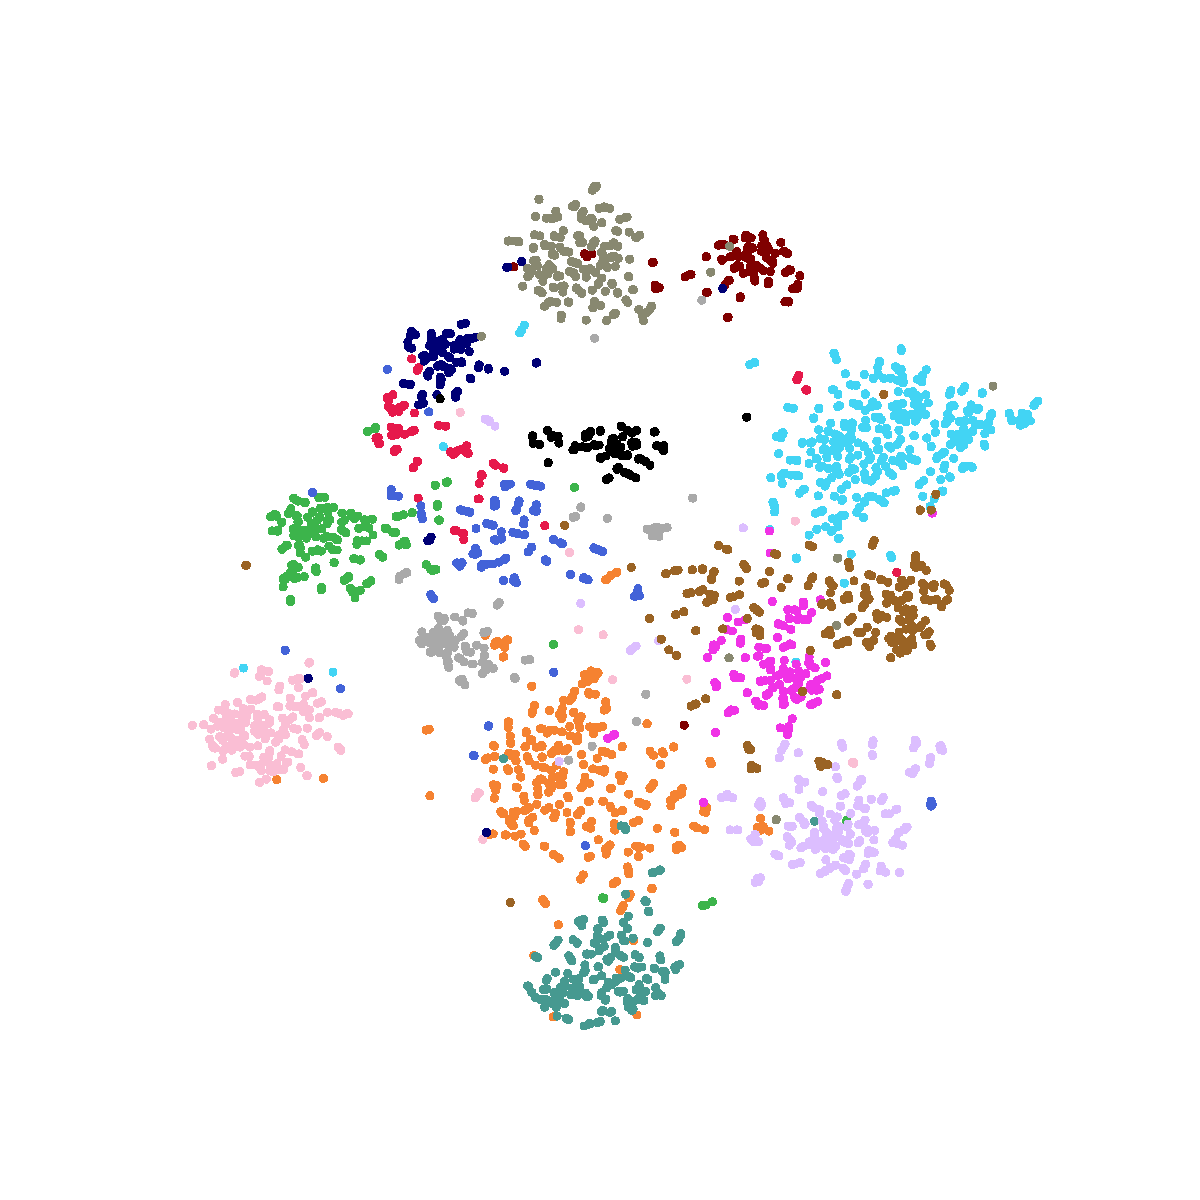
\includegraphics[width=\linewidth]{fig/tsne/point_mae.pdf}
        \caption*{\textbf{\#TP}:22.1M \textbf{\#OA}:85.18}
        \caption{Full fine-tuning}
        \label{fig:sub1}
    \end{subfigure}
    \hfill
    \begin{subfigure}{0.19\textwidth}
        \centering
        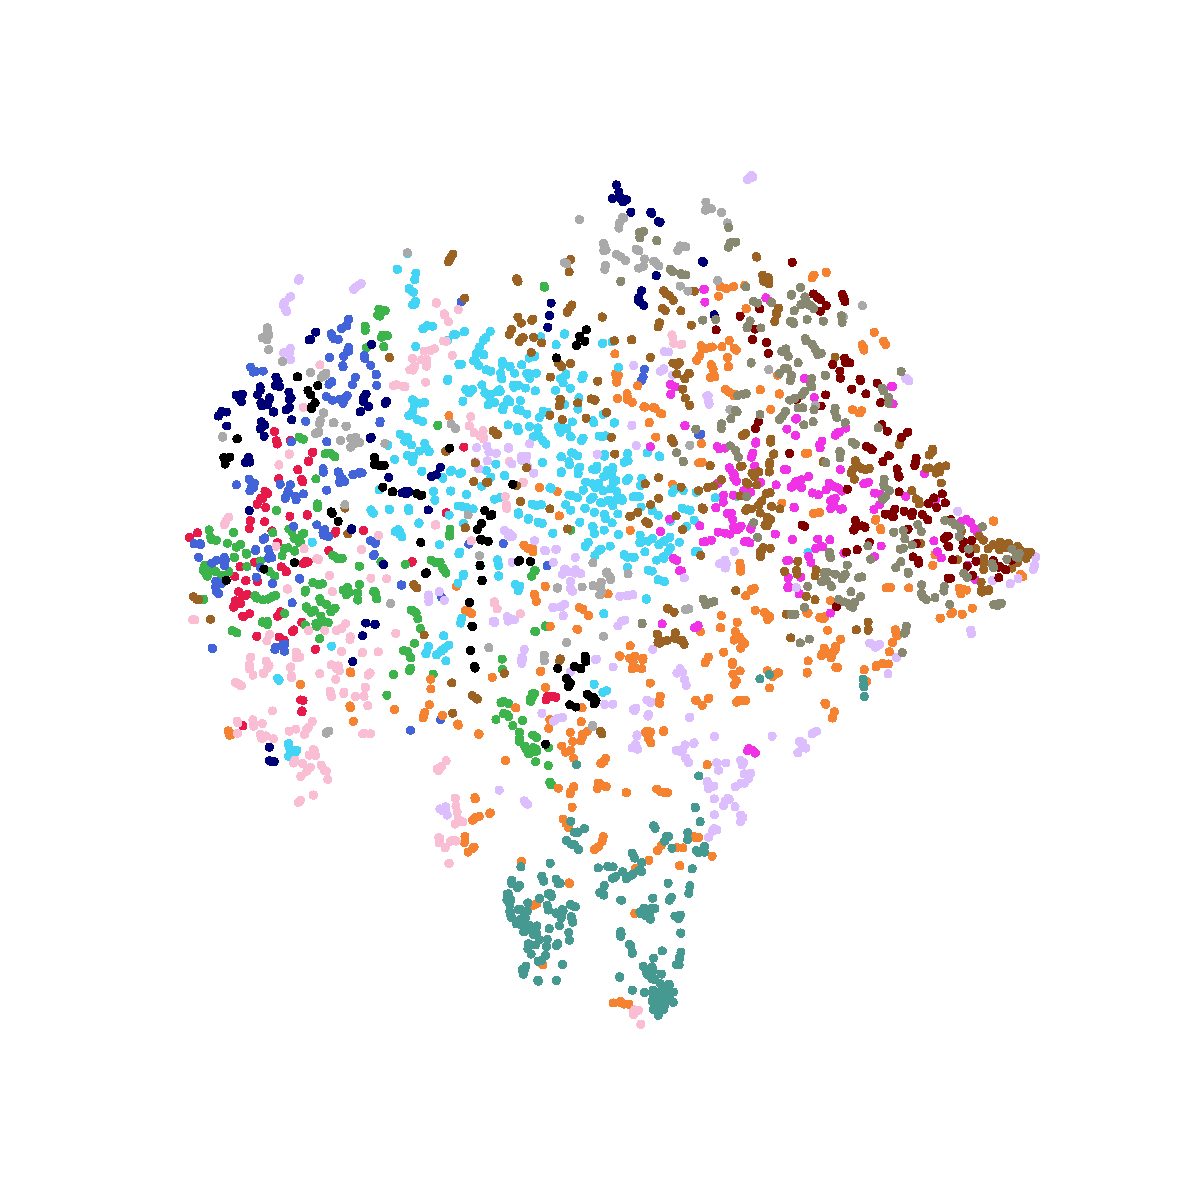
\includegraphics[width=\linewidth]{fig/tsne/LP.pdf}
        \caption*{\textbf{\#TP}:0.3M \textbf{\#OA}:75.99}
        \caption{Linear Probing}
        \label{fig:sub2}
    \end{subfigure}
    \hfill
    \begin{subfigure}{0.19\textwidth}
        \centering
        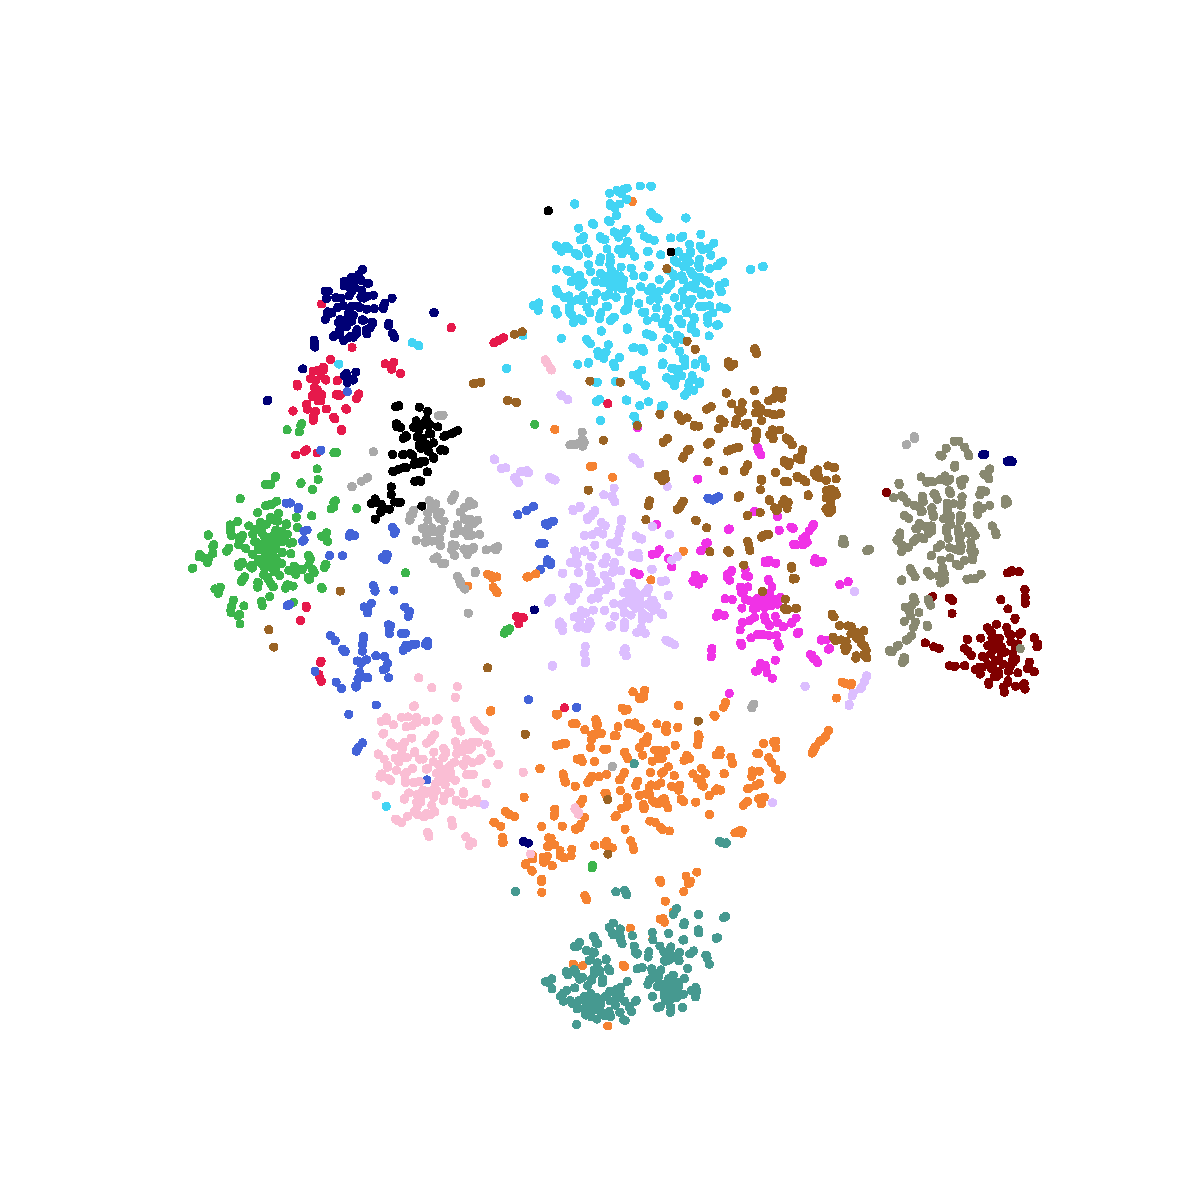
\includegraphics[width=\linewidth]{fig/tsne/idpt.pdf}
        \caption*{\textbf{\#TP}:1.7M \textbf{\#OA}:84.94}
        \caption{IDPT}
        \label{fig:sub3}
    \end{subfigure}
    \hfill
    \begin{subfigure}{0.19\textwidth}
        \centering
        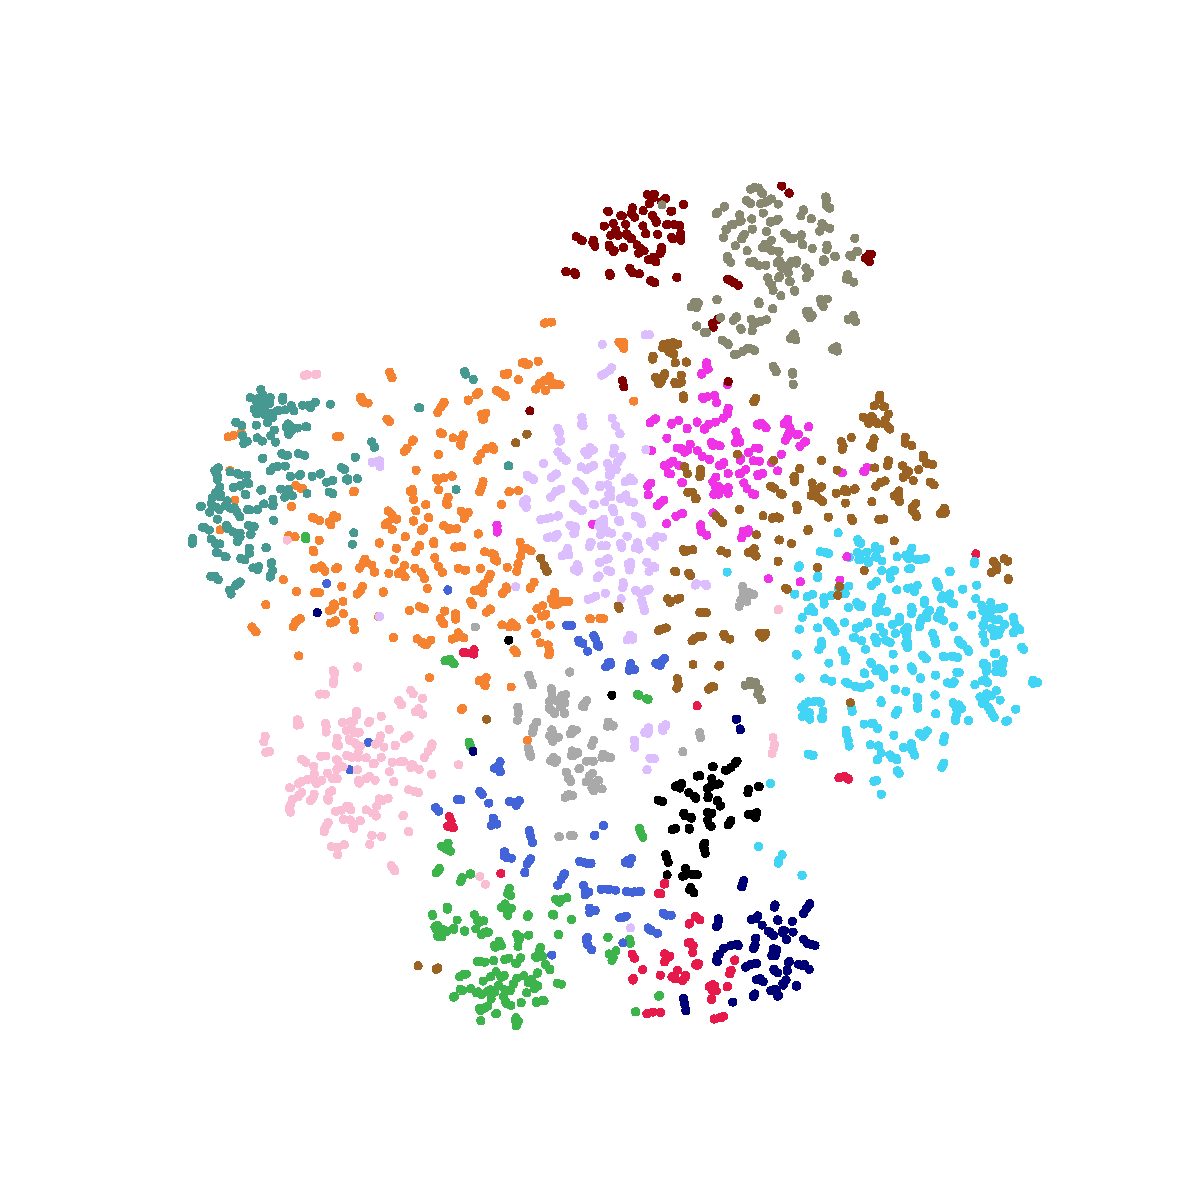
\includegraphics[width=\linewidth]{fig/tsne/dapt.pdf}
        \caption*{\textbf{\#TP}:1.1M \textbf{\#OA}:85.08}
        \caption{DAPT}
        \label{fig:sub4}
    \end{subfigure}
    % \hfill
    % \begin{subfigure}{0.24\textwidth}
    %     \centering
    %     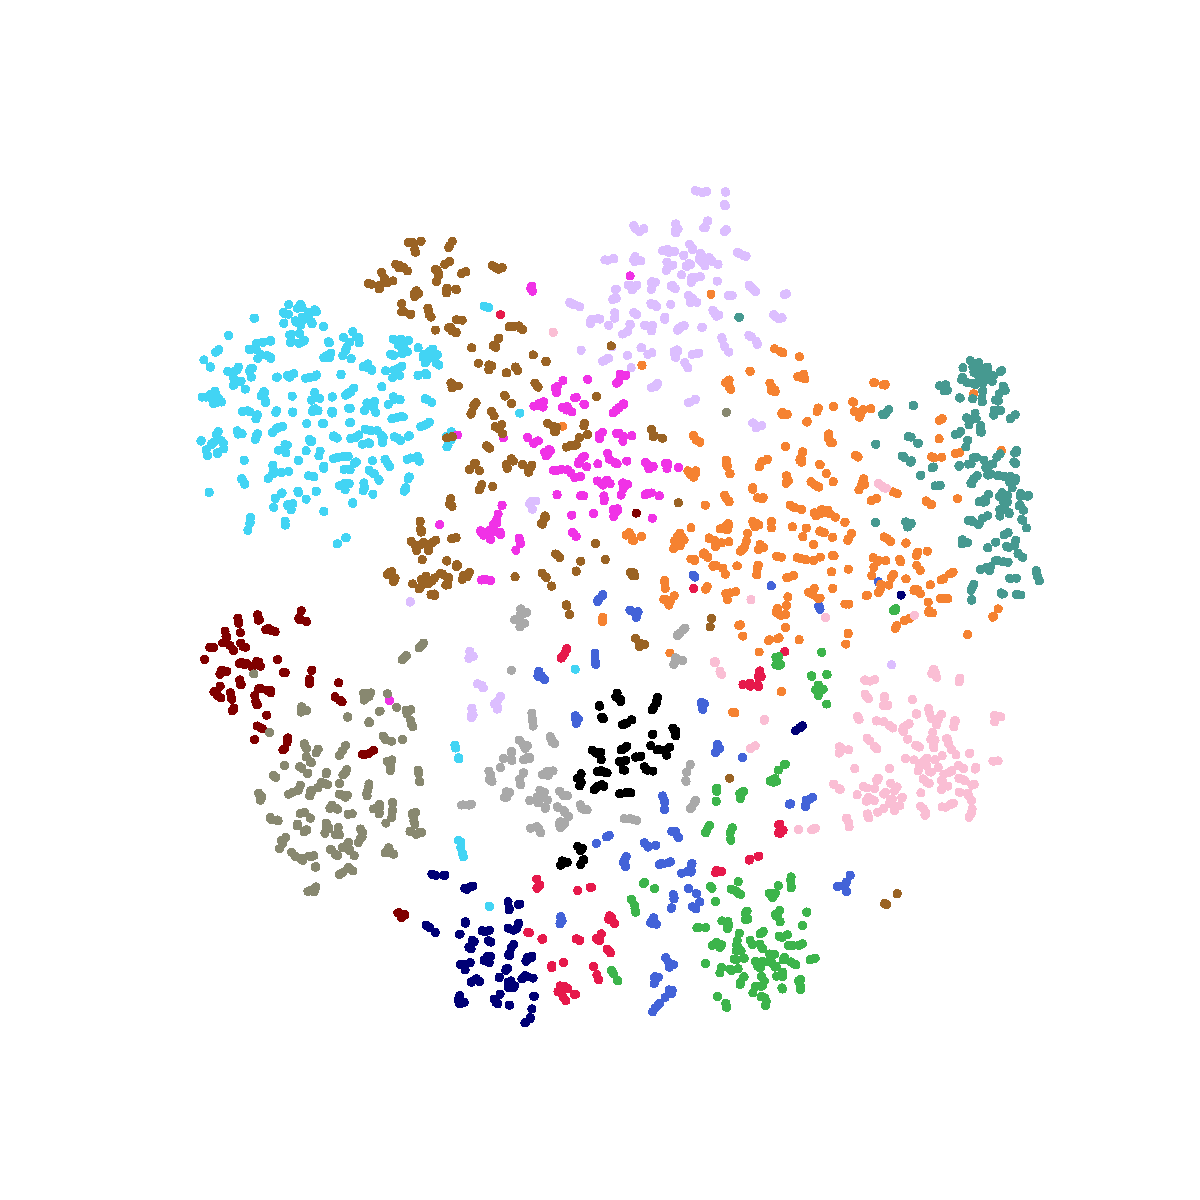
\includegraphics[width=\linewidth]{fig/tsne/pointgst.pdf}
    %     \caption*{\textbf{\#TP}:0.6M \textbf{\#OA}:85.29}
    %     \caption{PointGST}
    %     \label{fig:sub5}
    % \end{subfigure}
    % \hfill
    % \begin{subfigure}{0.24\textwidth}
    %     \centering
    %     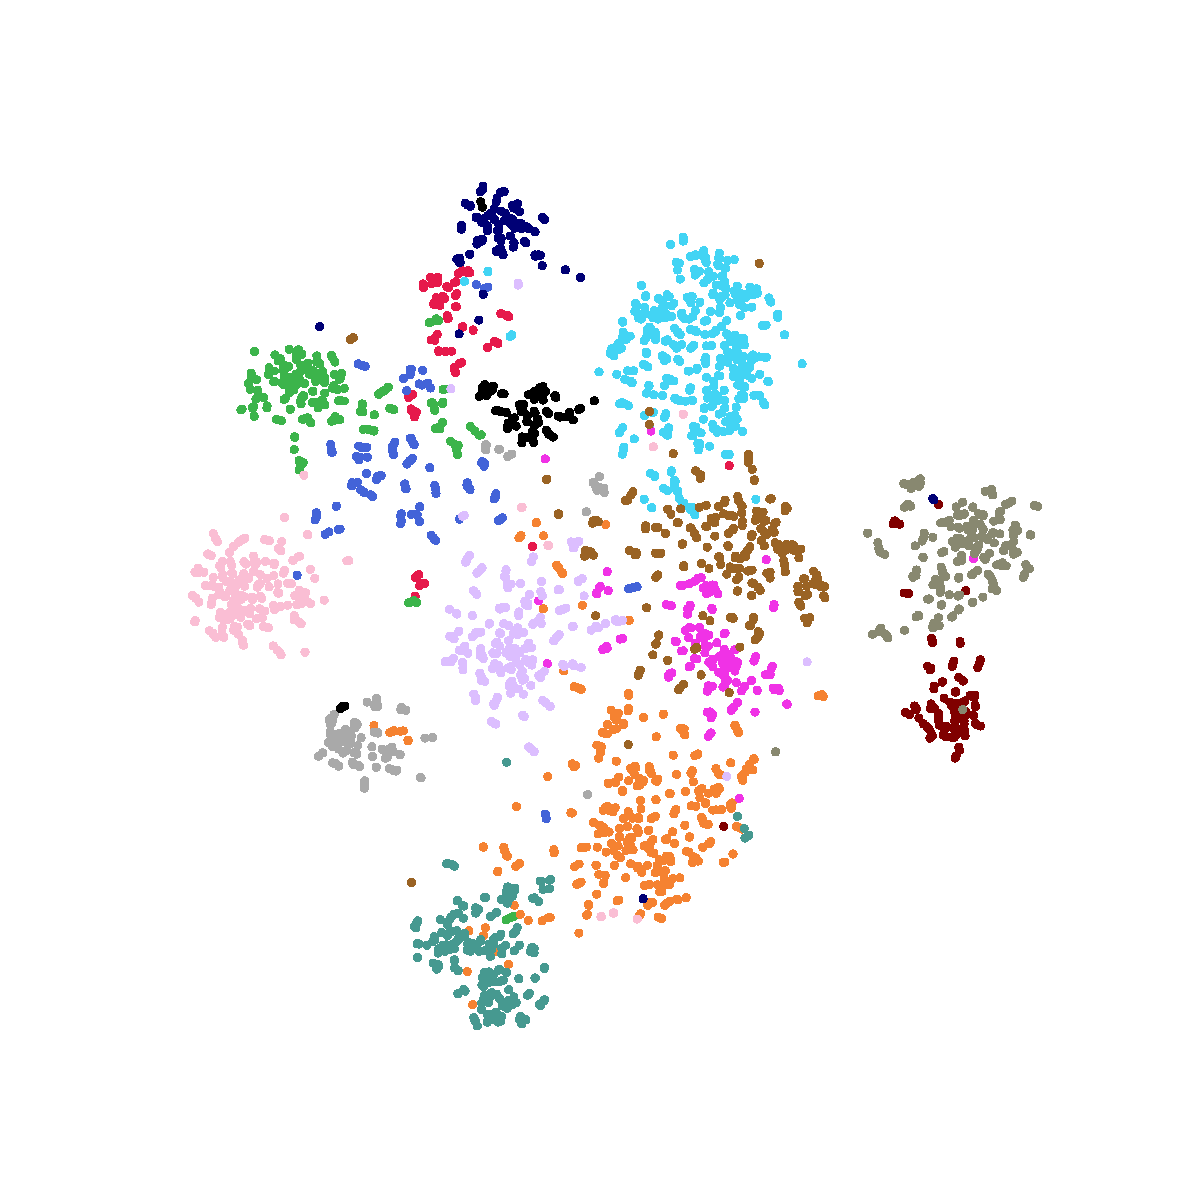
\includegraphics[width=\linewidth]{fig/tsne/PPT.pdf}
    %     \caption*{\textbf{\#TP}:1.1M \textbf{\#OA}:84.91}
    %     \caption{PPT}
    %     \label{fig:sub6}
    % \end{subfigure}
    % \hfill
    % \begin{subfigure}{0.24\textwidth}
    %     \centering
    %     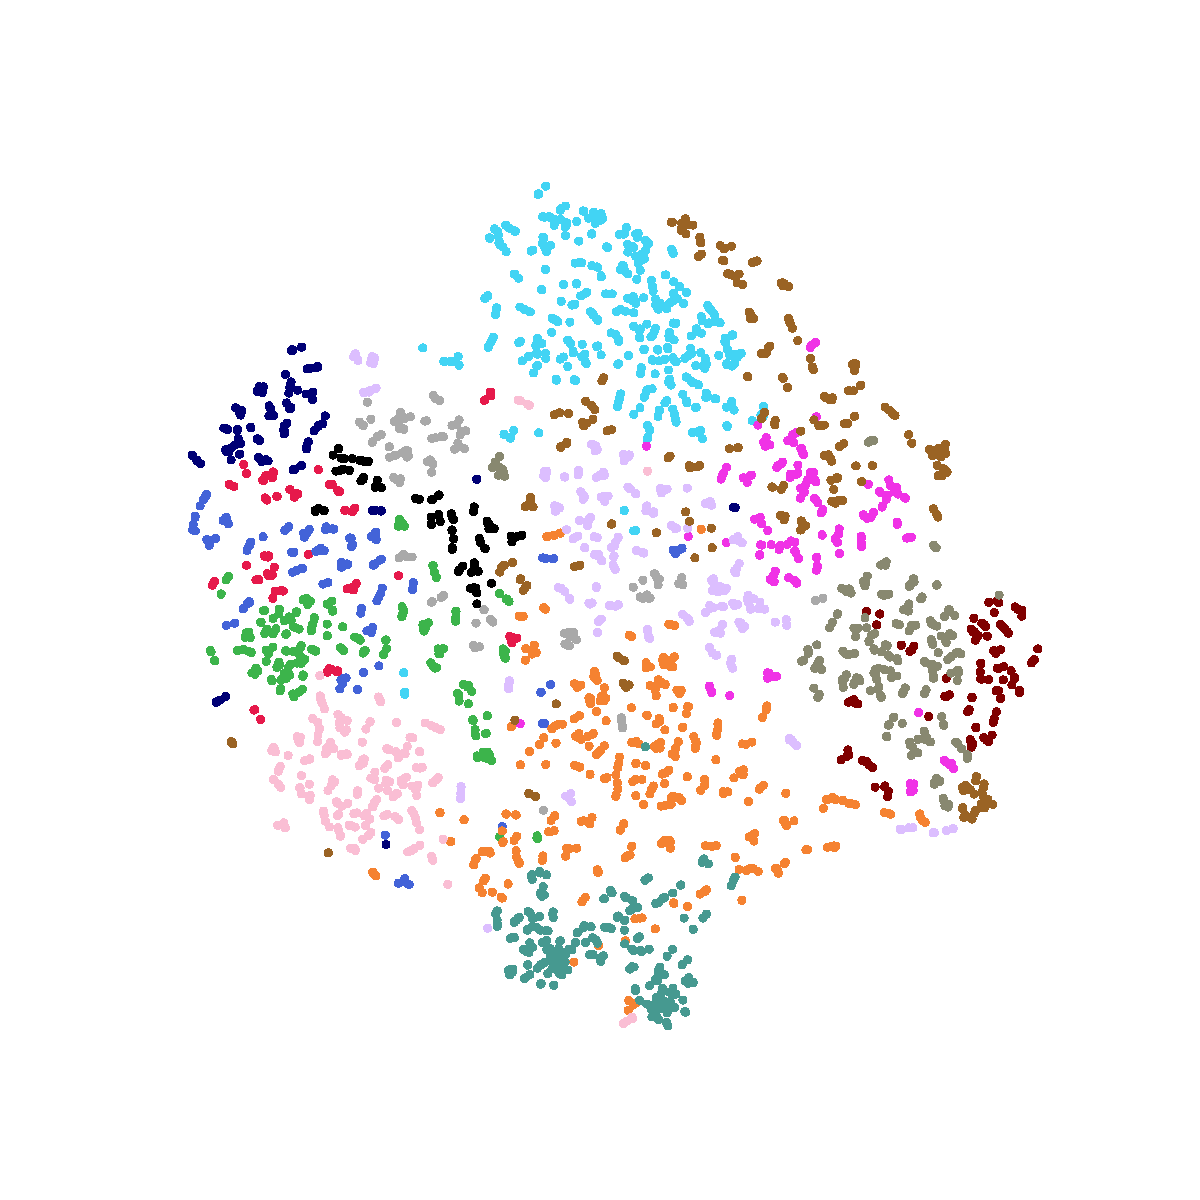
\includegraphics[width=\linewidth]{fig/tsne/LST.pdf}
    %     \caption*{\textbf{\#TP}:0.8M \textbf{\#OA}:82.75}
    %     \caption{LST}
    %     \label{fig:sub7}
    % \end{subfigure}
    \hfill
    \begin{subfigure}{0.19\textwidth}
        \centering
        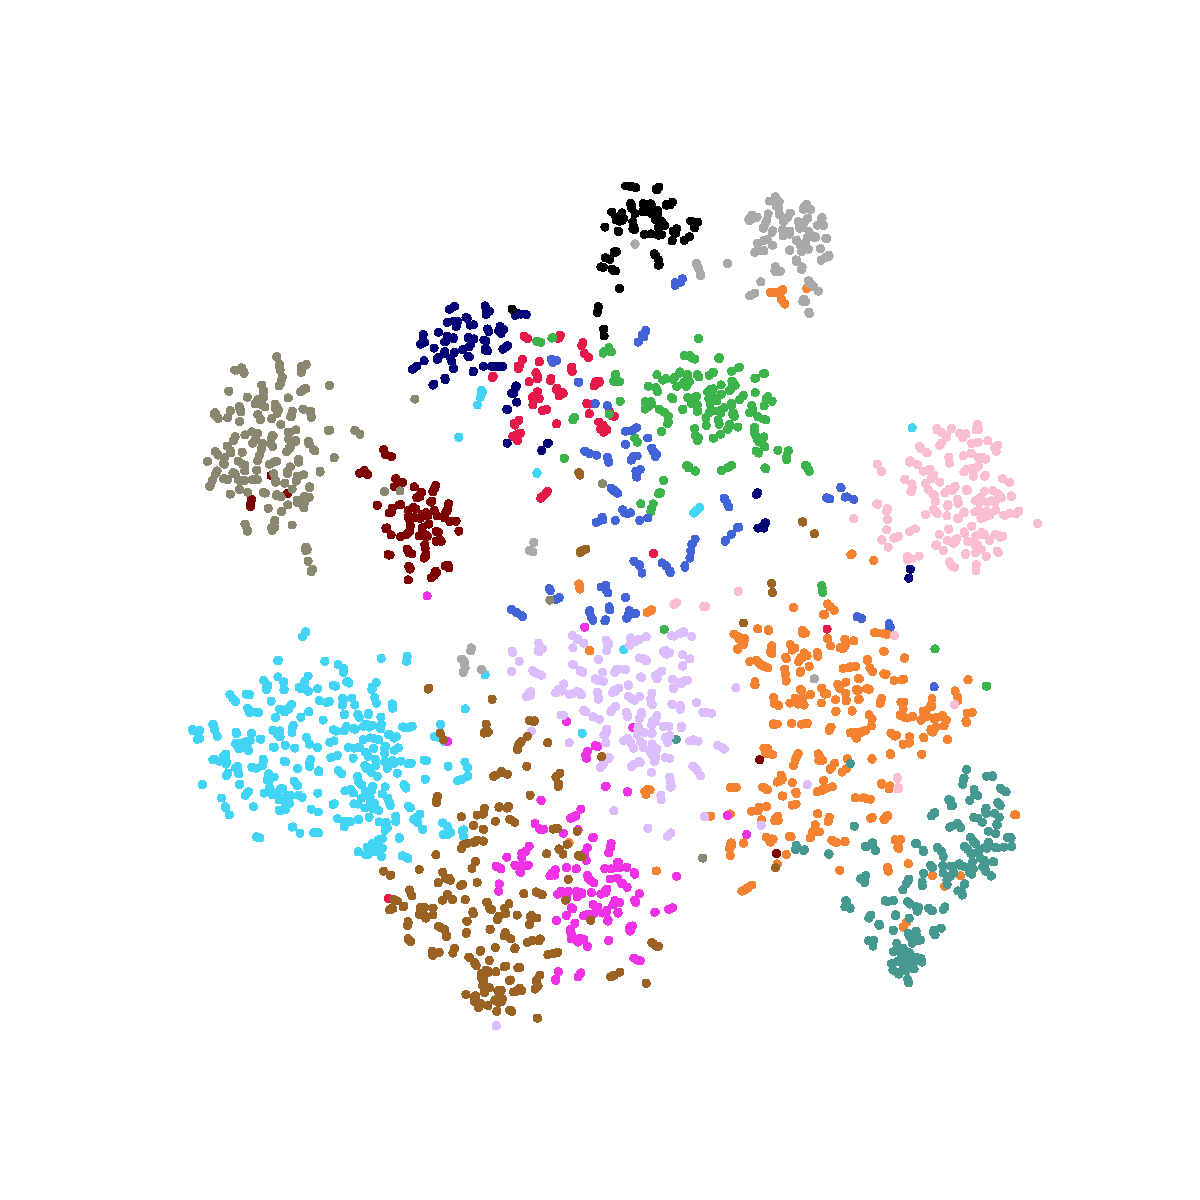
\includegraphics[width=\linewidth]{fig/tsne/point_ladder.pdf}
        \caption*{\textbf{\#TP}:0.6M \textbf{\#OA}:85.53}
        \caption{PLT (Ours)}
        \label{fig:sub8}
    \end{subfigure}
    \caption{The visualization of the t-SNE~\cite{van2008visualizing} from the test sets of ScanObjectNN~\cite{uy2019revisiting} (PB\_T50\_RS) by using a pre-trained PointMAE~\cite{pang2022masked} with various fine-tuning strategies. We extract the final classification features from the top linear layer for t-SNE visualizations.}
    \label{fig:tsne}
\end{figure*}

\begin{figure*}
    \centering
    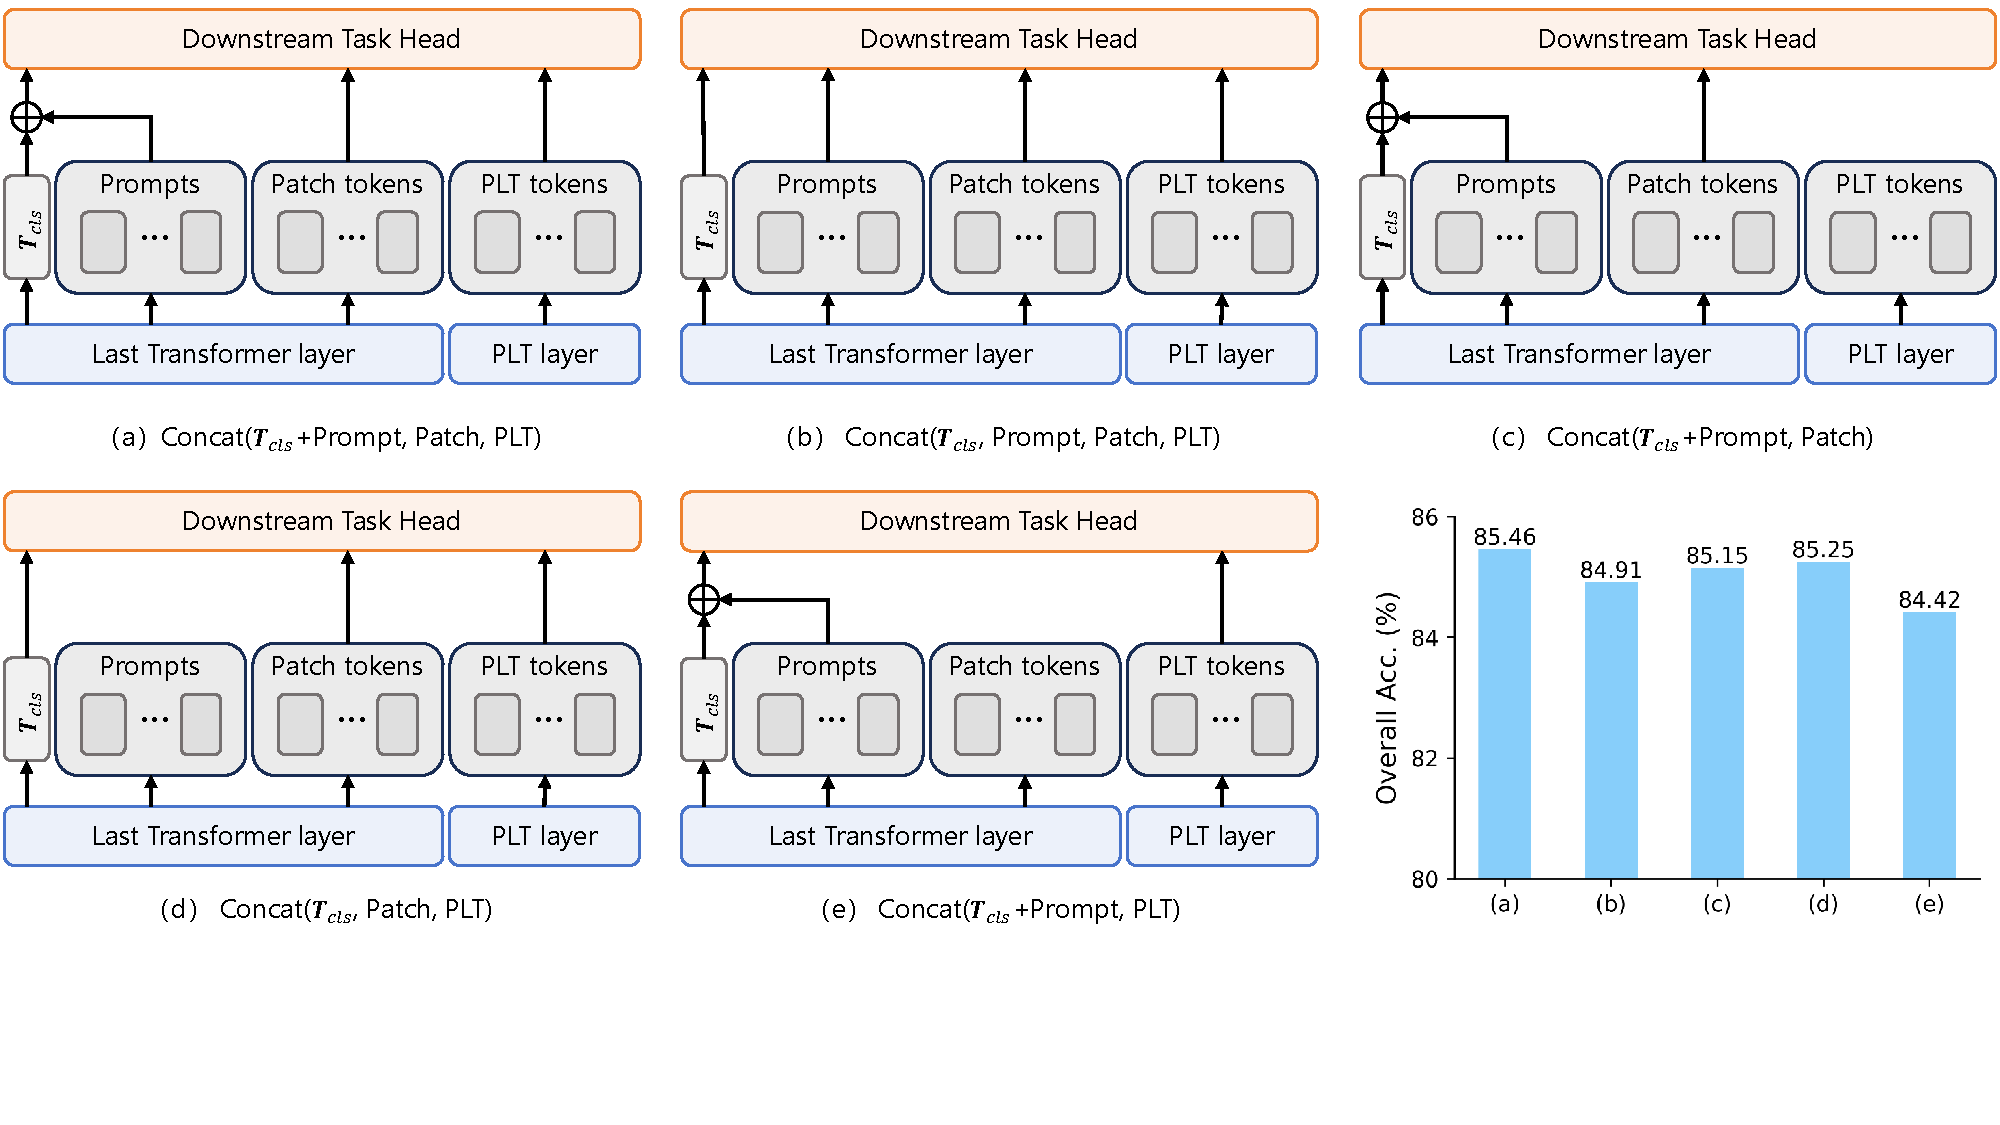
\includegraphics[width=\linewidth]{fig/Effect of different inputs for downstream task head.pdf}
    \caption{Effect of different inputs for downstream classification task head. We conduct experiments on the hardest variant (i.e., PB\_T50\_RS) of ScanObjectNN~\cite{uy2019revisiting} with Point-MAE baseline~\cite{pang2022masked}.}
    \label{fig:whole}
\end{figure*}
\begin{figure*}
    \centering
    \begin{subfigure}{0.46\textwidth}
        \centering
        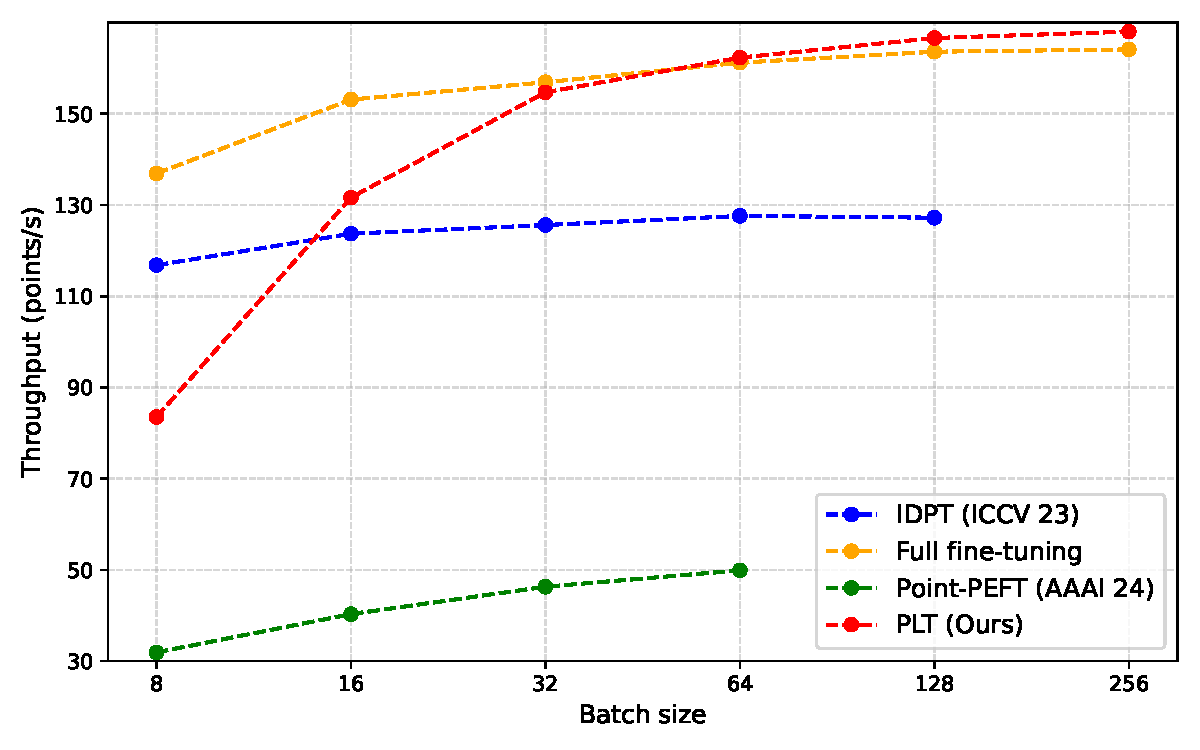
\includegraphics[width=\linewidth]{fig/supplement/performance/train_speed.pdf}
        \caption{Train Speed}
        \label{fig:per1}
    \end{subfigure}
    \hfill
    \begin{subfigure}{0.46\textwidth}
        \centering
        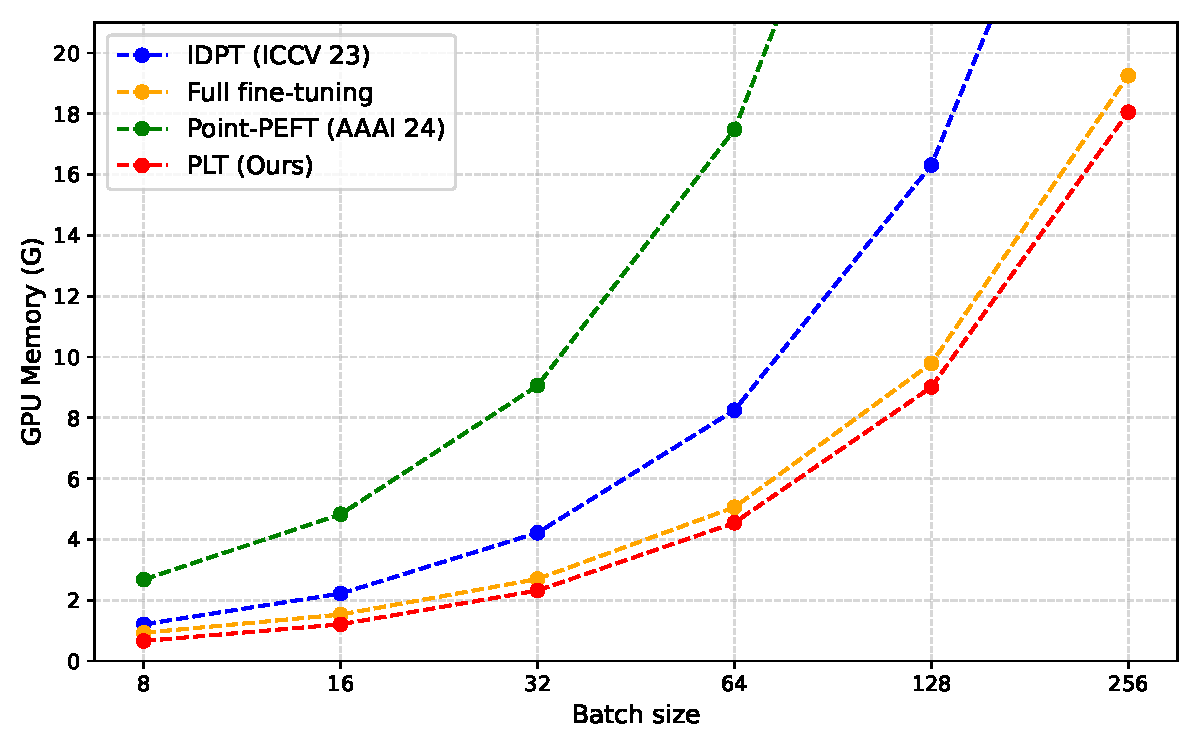
\includegraphics[width=\linewidth]{fig/supplement/performance/train_memory.pdf}
        \caption{Train Memory}
        \label{fig:per2}
    \end{subfigure}
    \hfill
    \begin{subfigure}{0.46\textwidth}
        \centering
        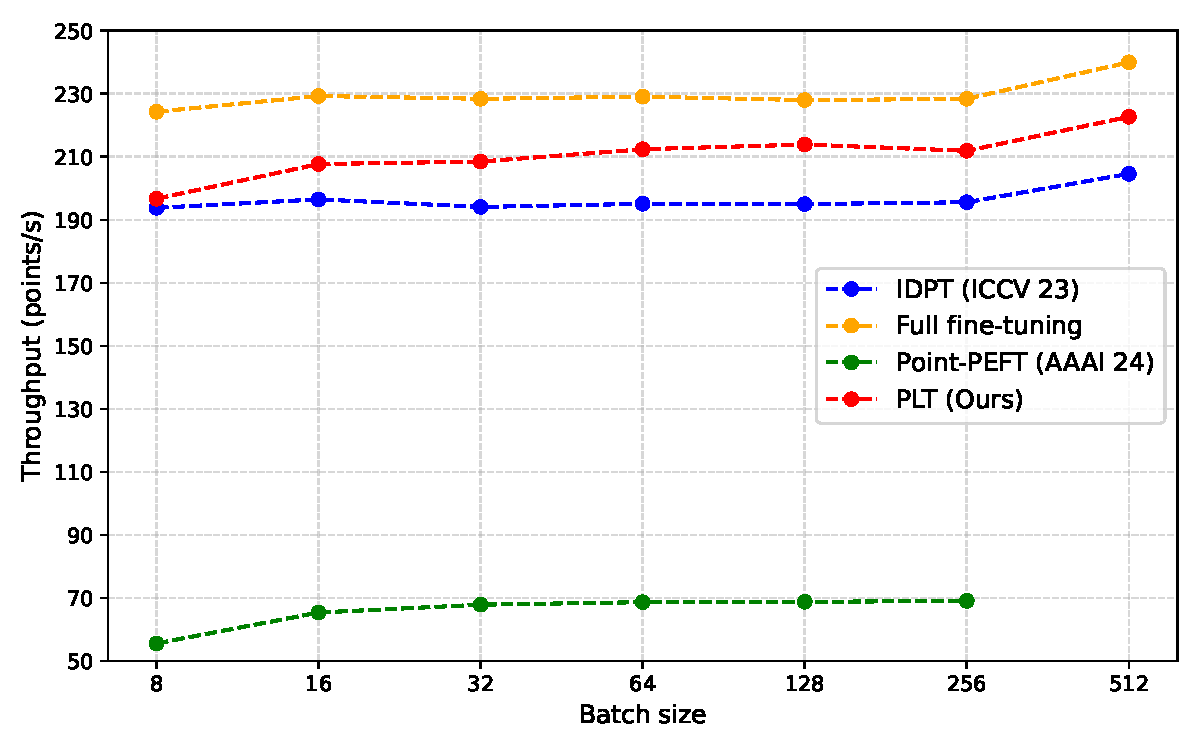
\includegraphics[width=\linewidth]{fig/supplement/performance/infer_speed.pdf}
        \caption{Infer Speed}
        \label{fig:per3}
    \end{subfigure}
    \hfill
    \begin{subfigure}{0.46\textwidth}
        \centering
        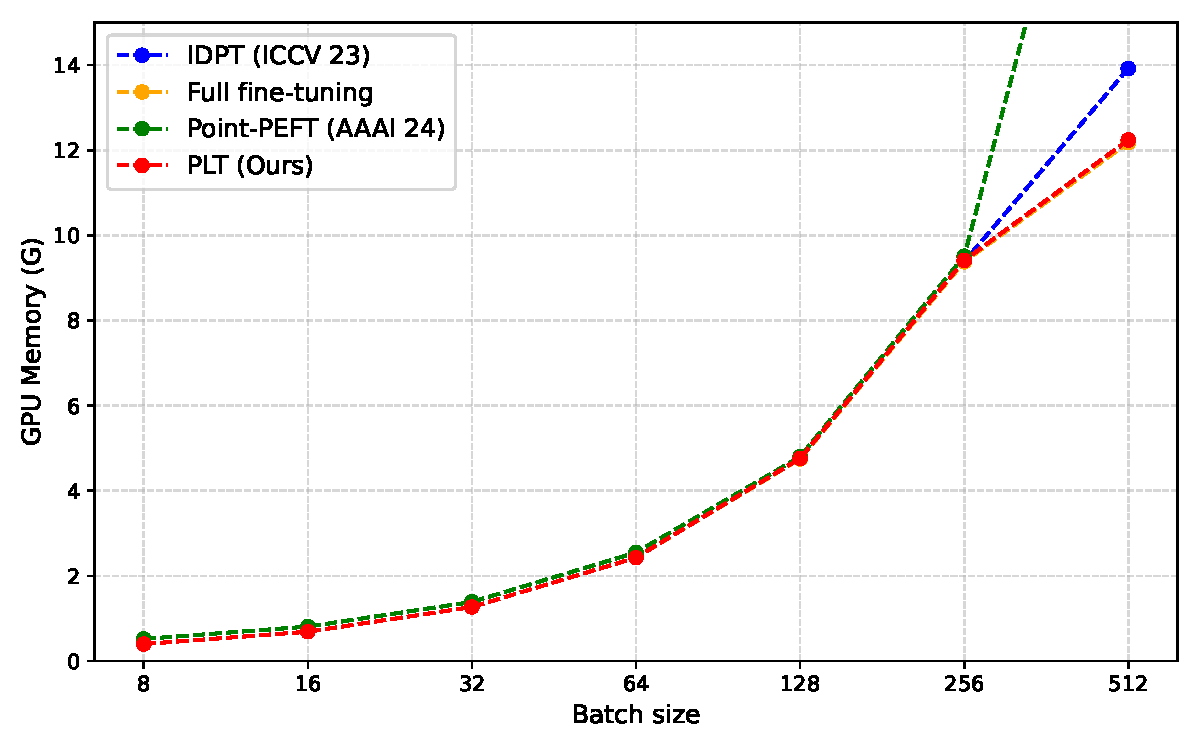
\includegraphics[width=\linewidth]{fig/supplement/performance/infer_memory.pdf}
        \caption{Infer Memory}
        \label{fig:per4}
    \end{subfigure}
    \hfill
    \caption{Comparison of performance between Our PLT and previous methods. We conduct experiments on the hardest variant (i.e., PB\_T50\_RS) of ScanObjectNN~\cite{uy2019revisiting} with Point-MAE baseline~\cite{pang2022masked}. Throughput is measured on a single RTX 3090 GPU.}
    \label{fig:performance}
\end{figure*}

\begin{figure*}[htbp]
    \centering

    % 第一行左侧的竖排标签
    \begin{minipage}{0.1\textwidth}
        \centering
        {airplane}
        % \rotatebox{90}{14}
    \end{minipage}
    \hfill
    % 第一行图片
    \begin{minipage}{0.25\textwidth}
        \centering
        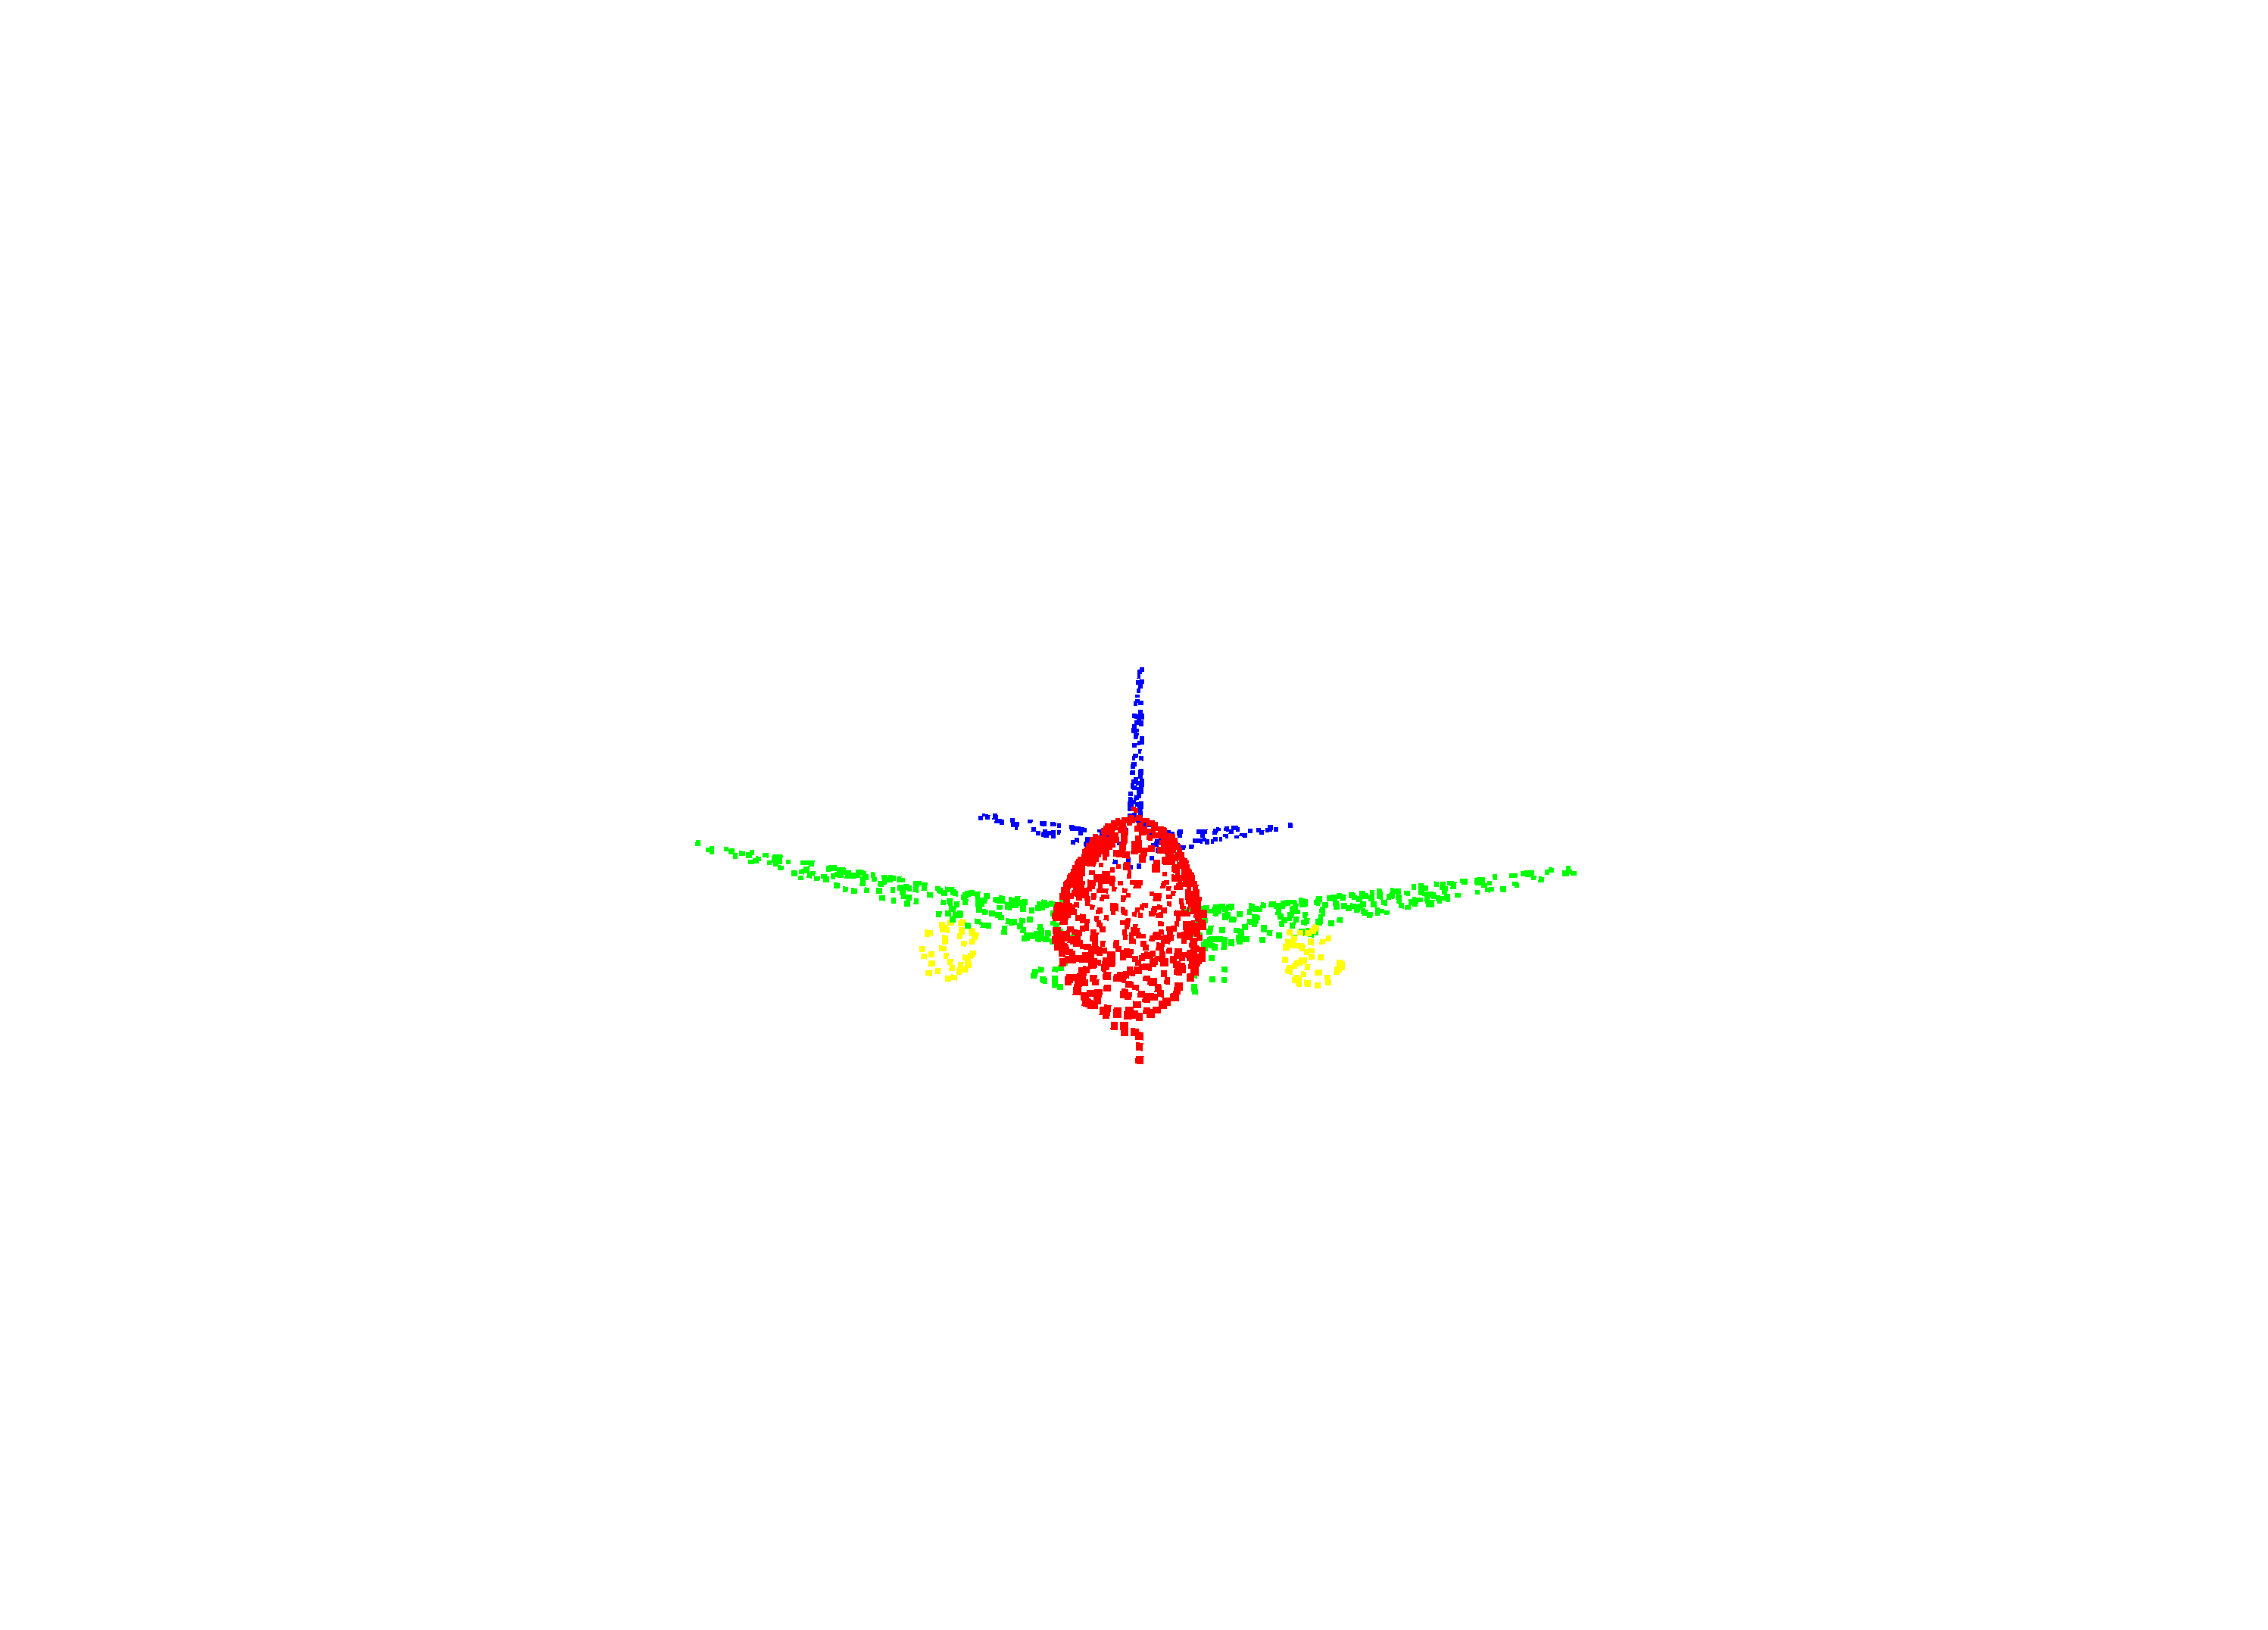
\includegraphics[width=\textwidth]{fig/supplement/part_segmentation/airplane/airplane00.pdf} % 替换为你的图片路径
    \end{minipage}
    \hfill
    \begin{minipage}{0.25\textwidth}
        \centering
        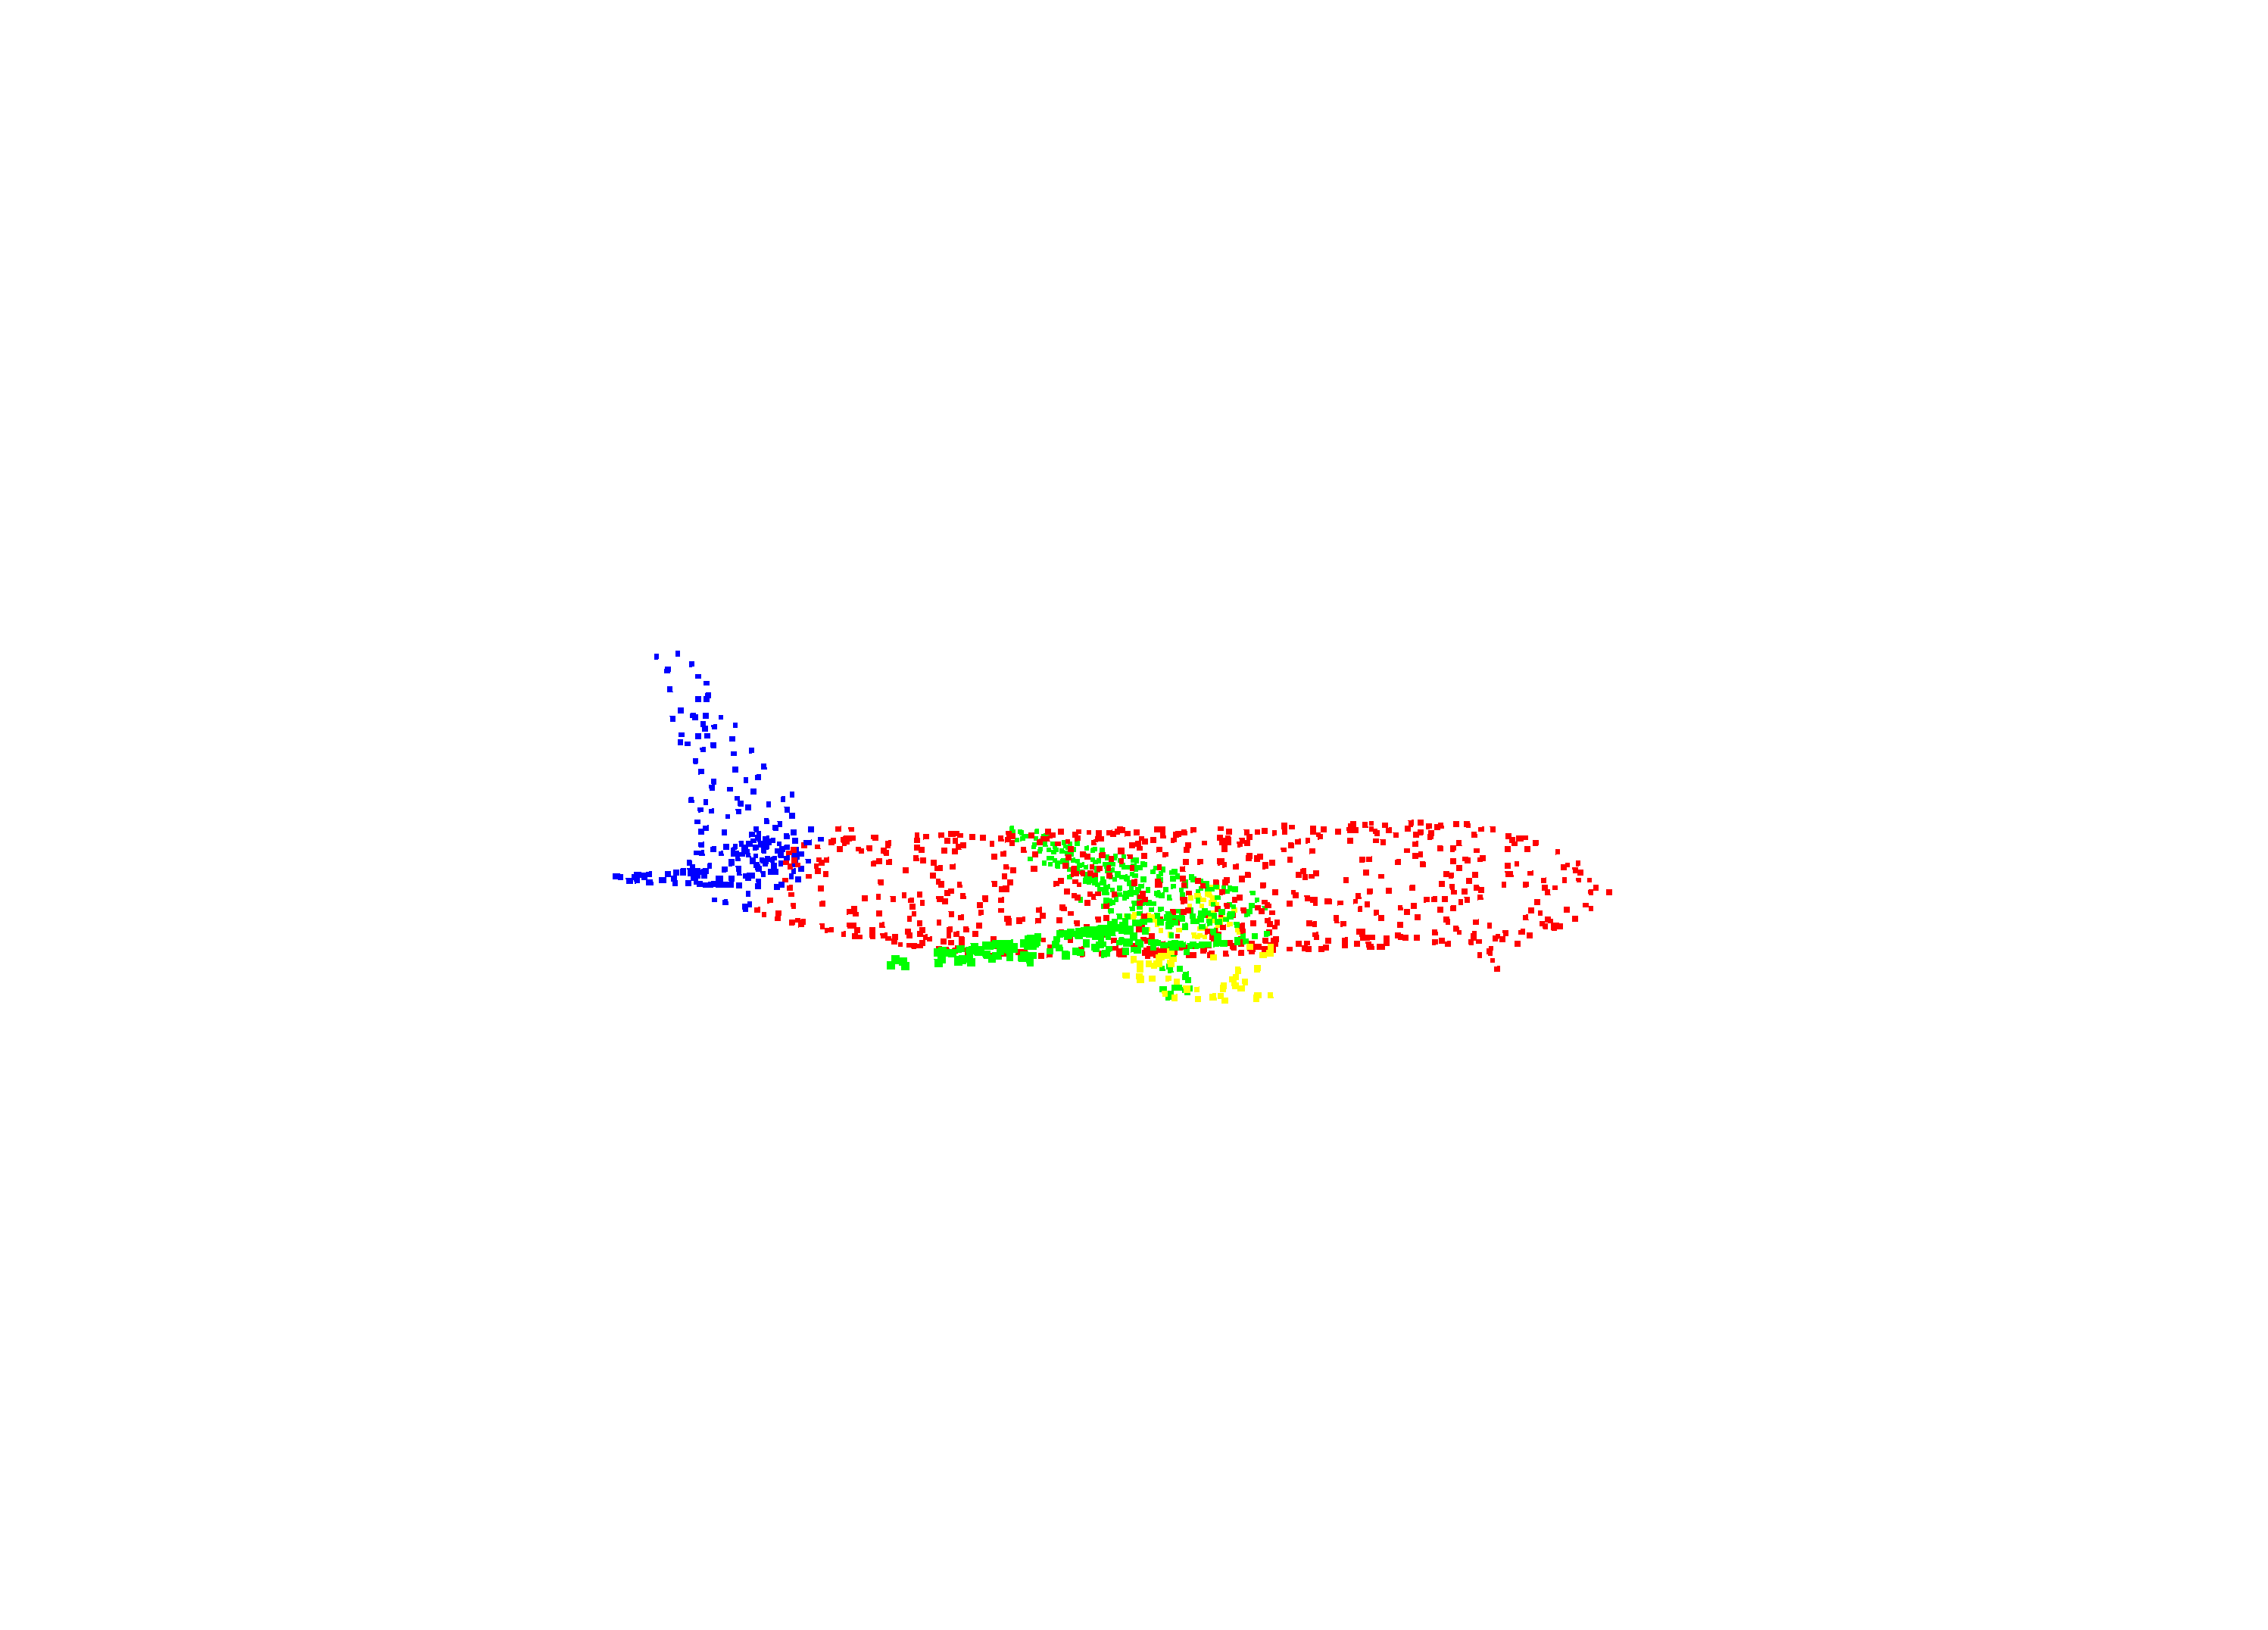
\includegraphics[width=\textwidth]{fig/supplement/part_segmentation/airplane/airplane01.pdf}
    \end{minipage}
    \hfill
    \begin{minipage}{0.25\textwidth}
        \centering
        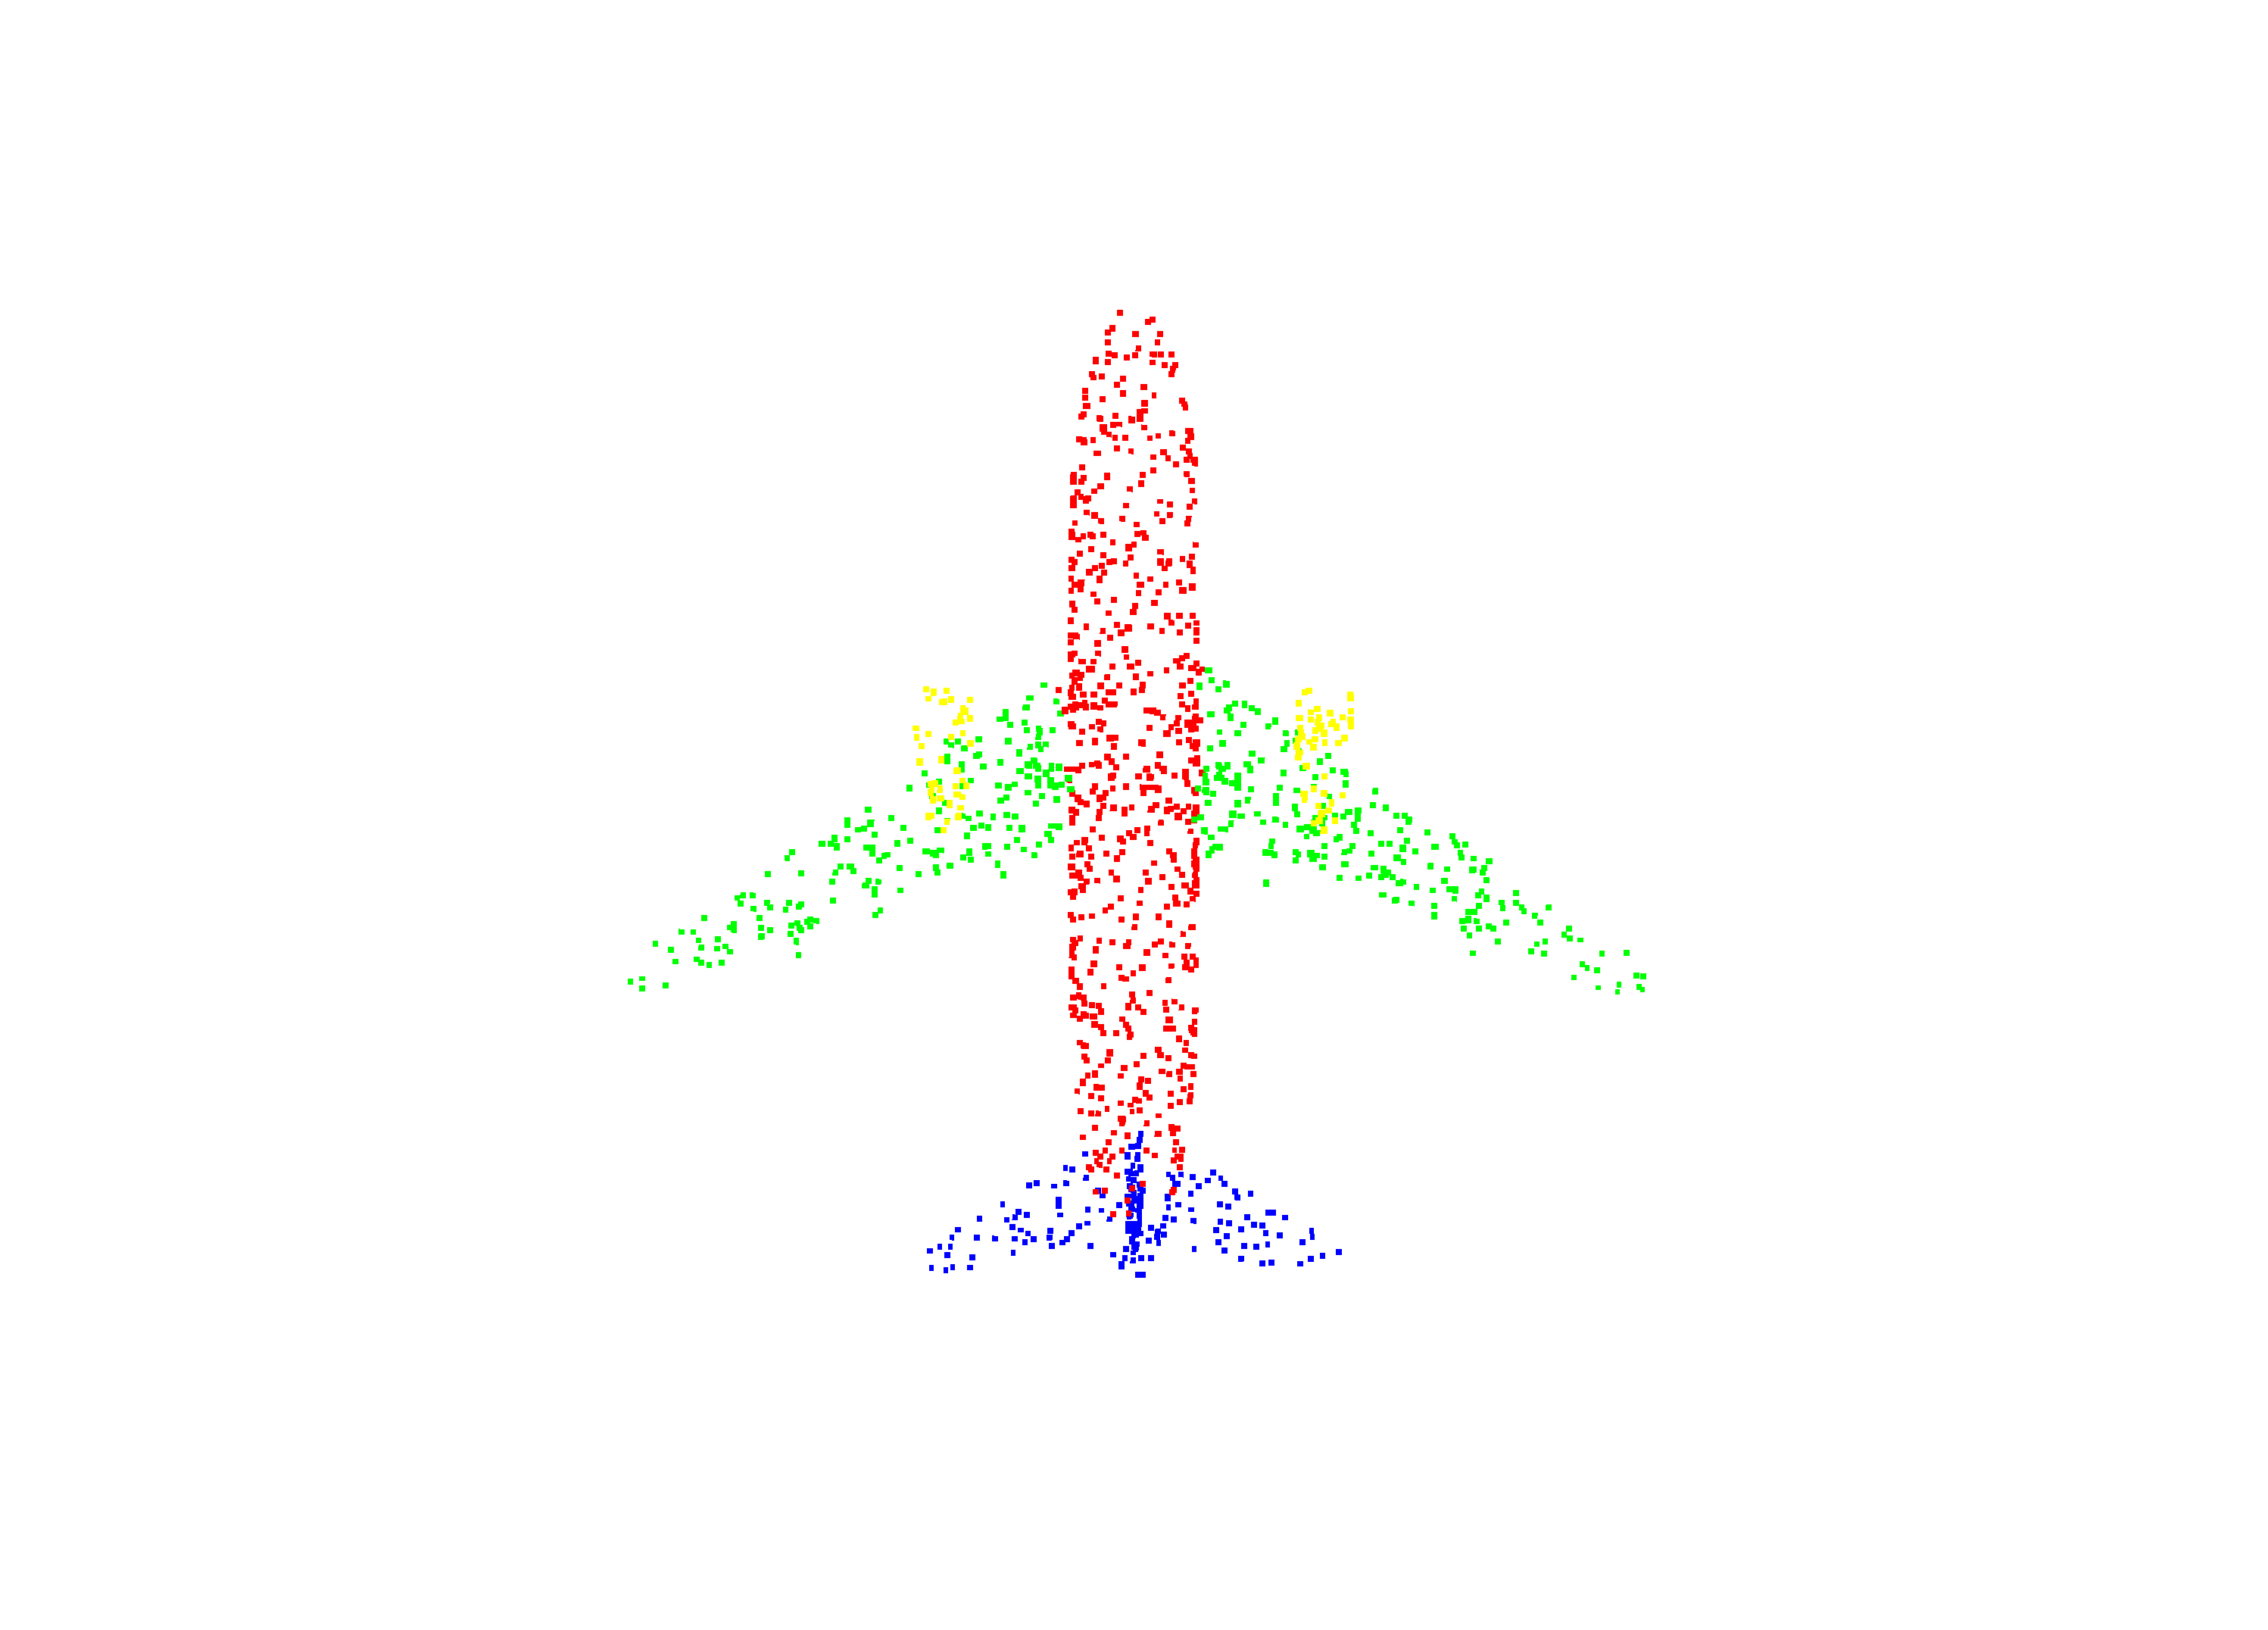
\includegraphics[width=\textwidth]{fig/supplement/part_segmentation/airplane/airplane02.pdf}
    \end{minipage}
    \hfill

    % 换行
    \vspace{0.5em}

    % 第二行左侧的竖排标签
    \begin{minipage}{0.1\textwidth}
        \centering
        {chair}
    \end{minipage}
    \hfill
    % 第二行图片
    \begin{minipage}{0.25\textwidth}
        \centering
        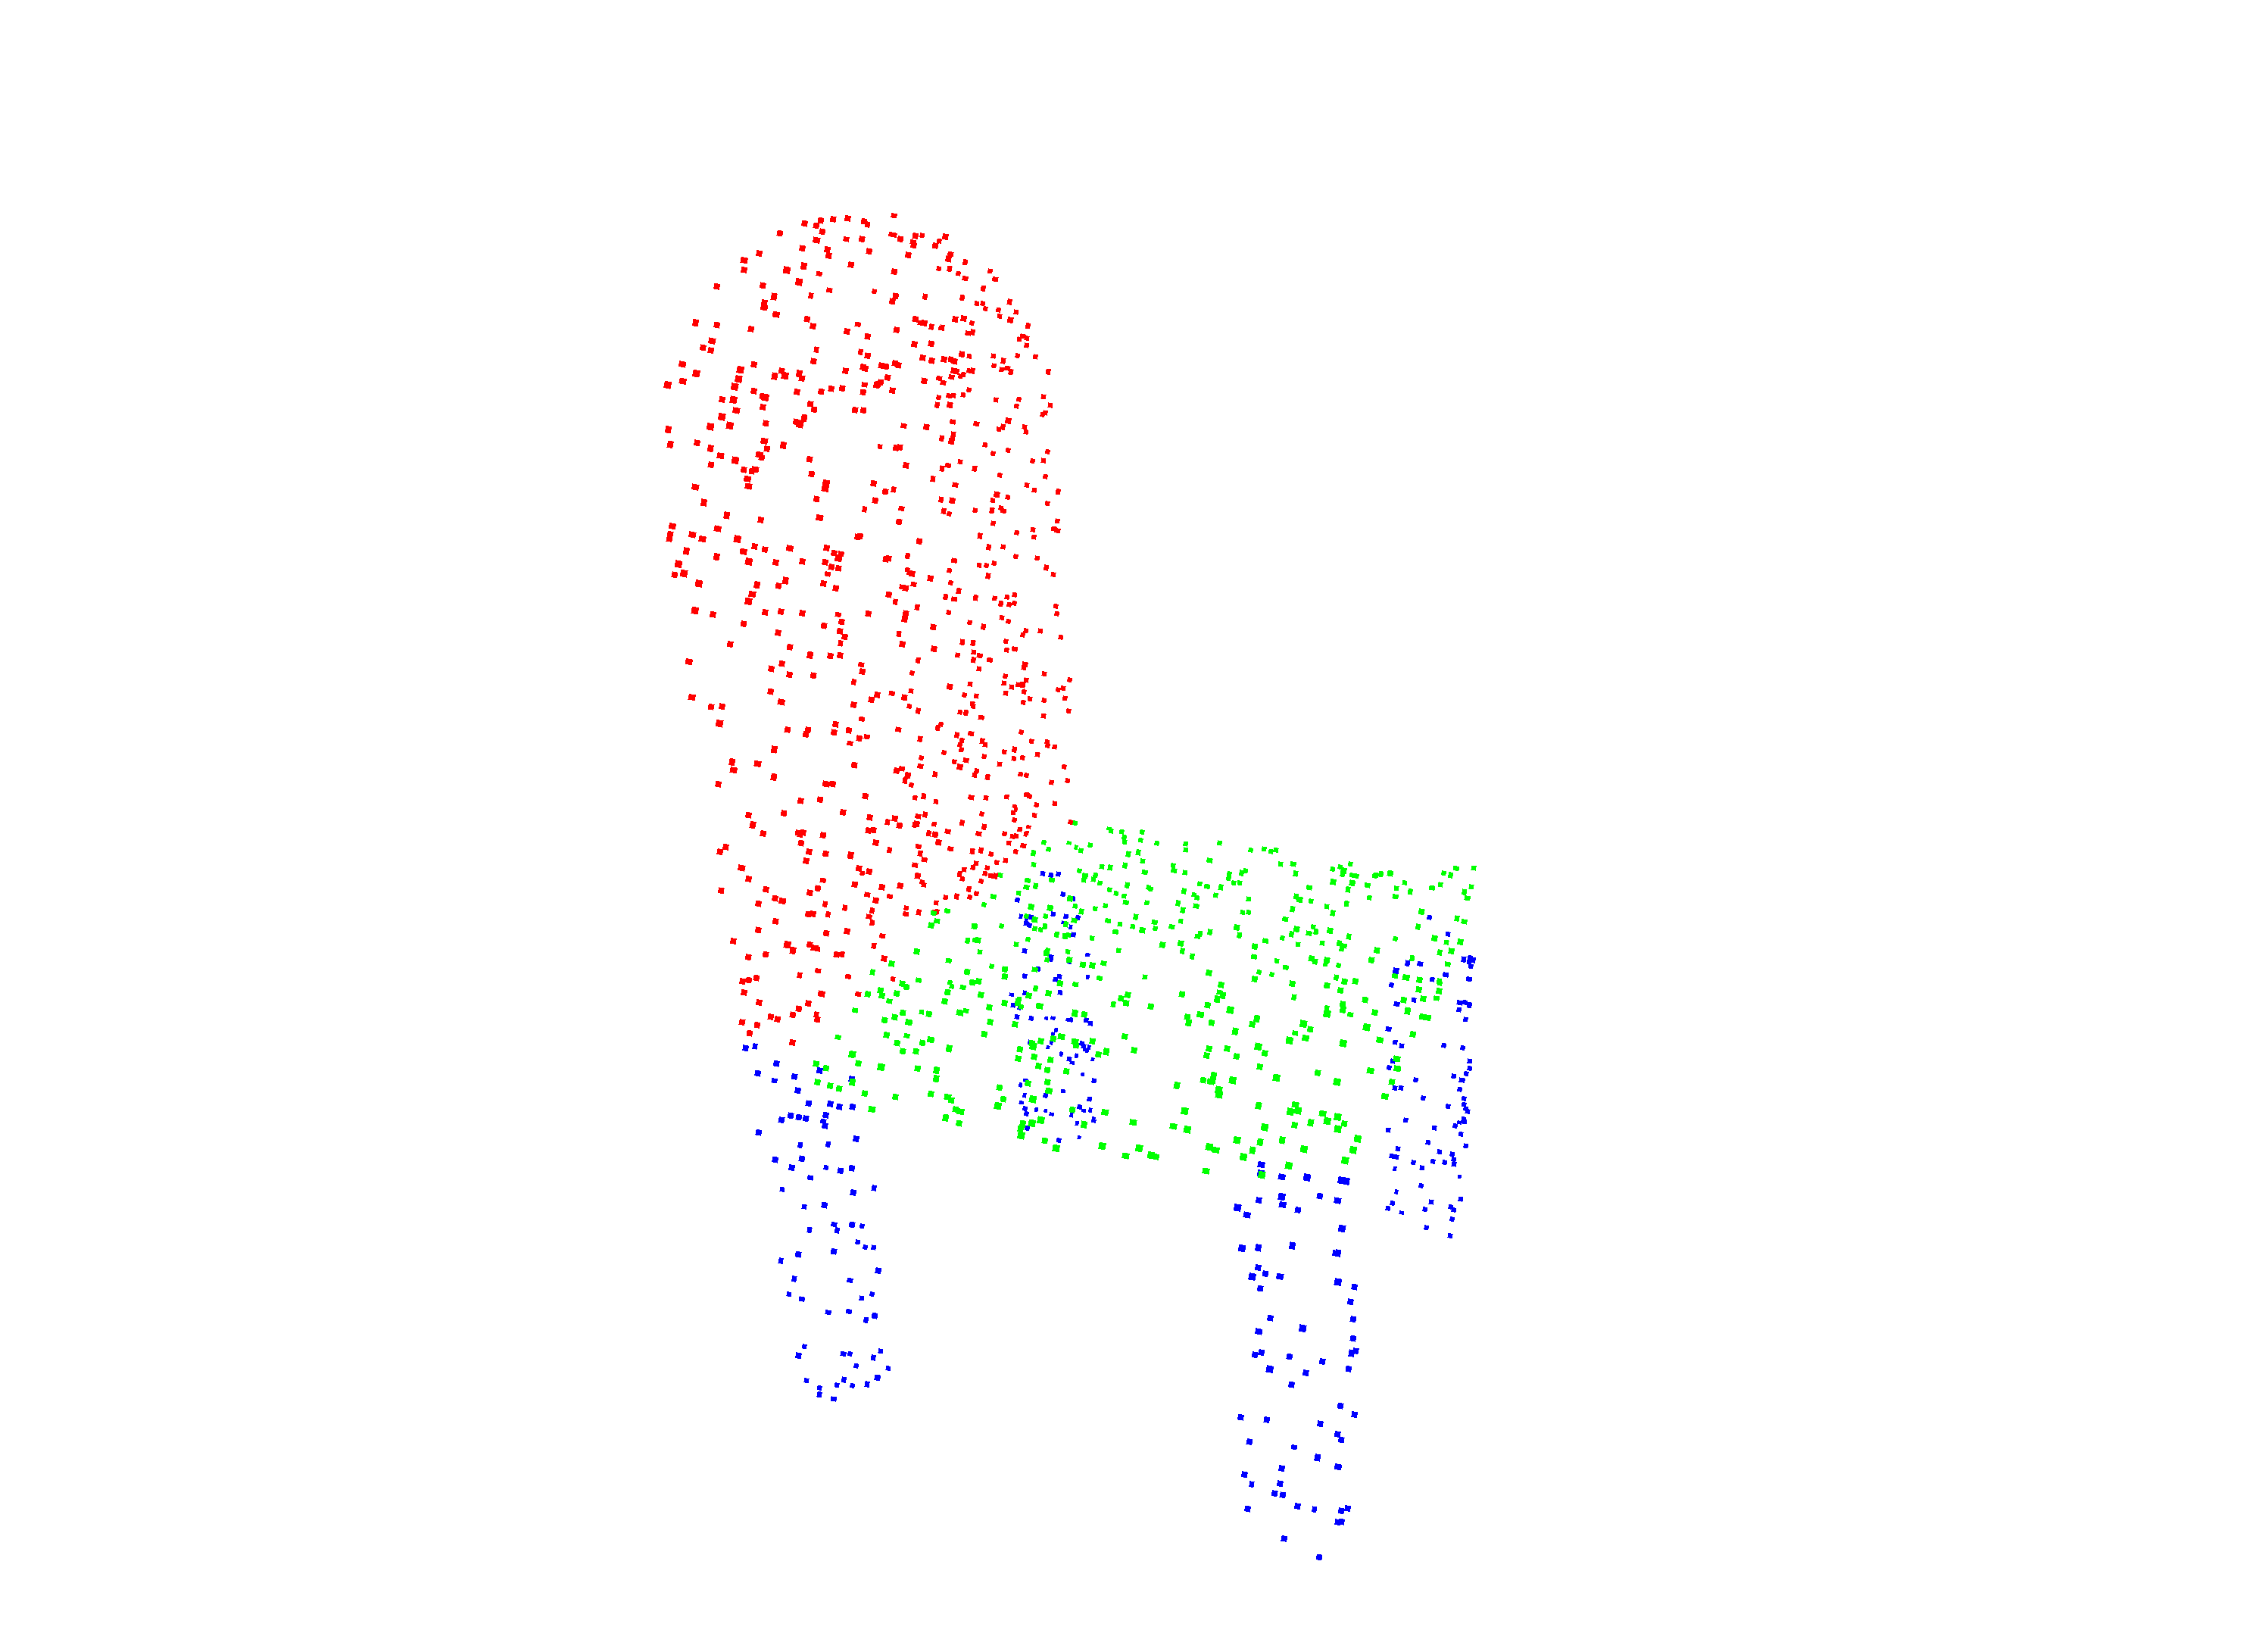
\includegraphics[width=\textwidth]{fig/supplement/part_segmentation/chair/chair00.pdf}
    \end{minipage}
    \hfill
    \begin{minipage}{0.25\textwidth}
        \centering
        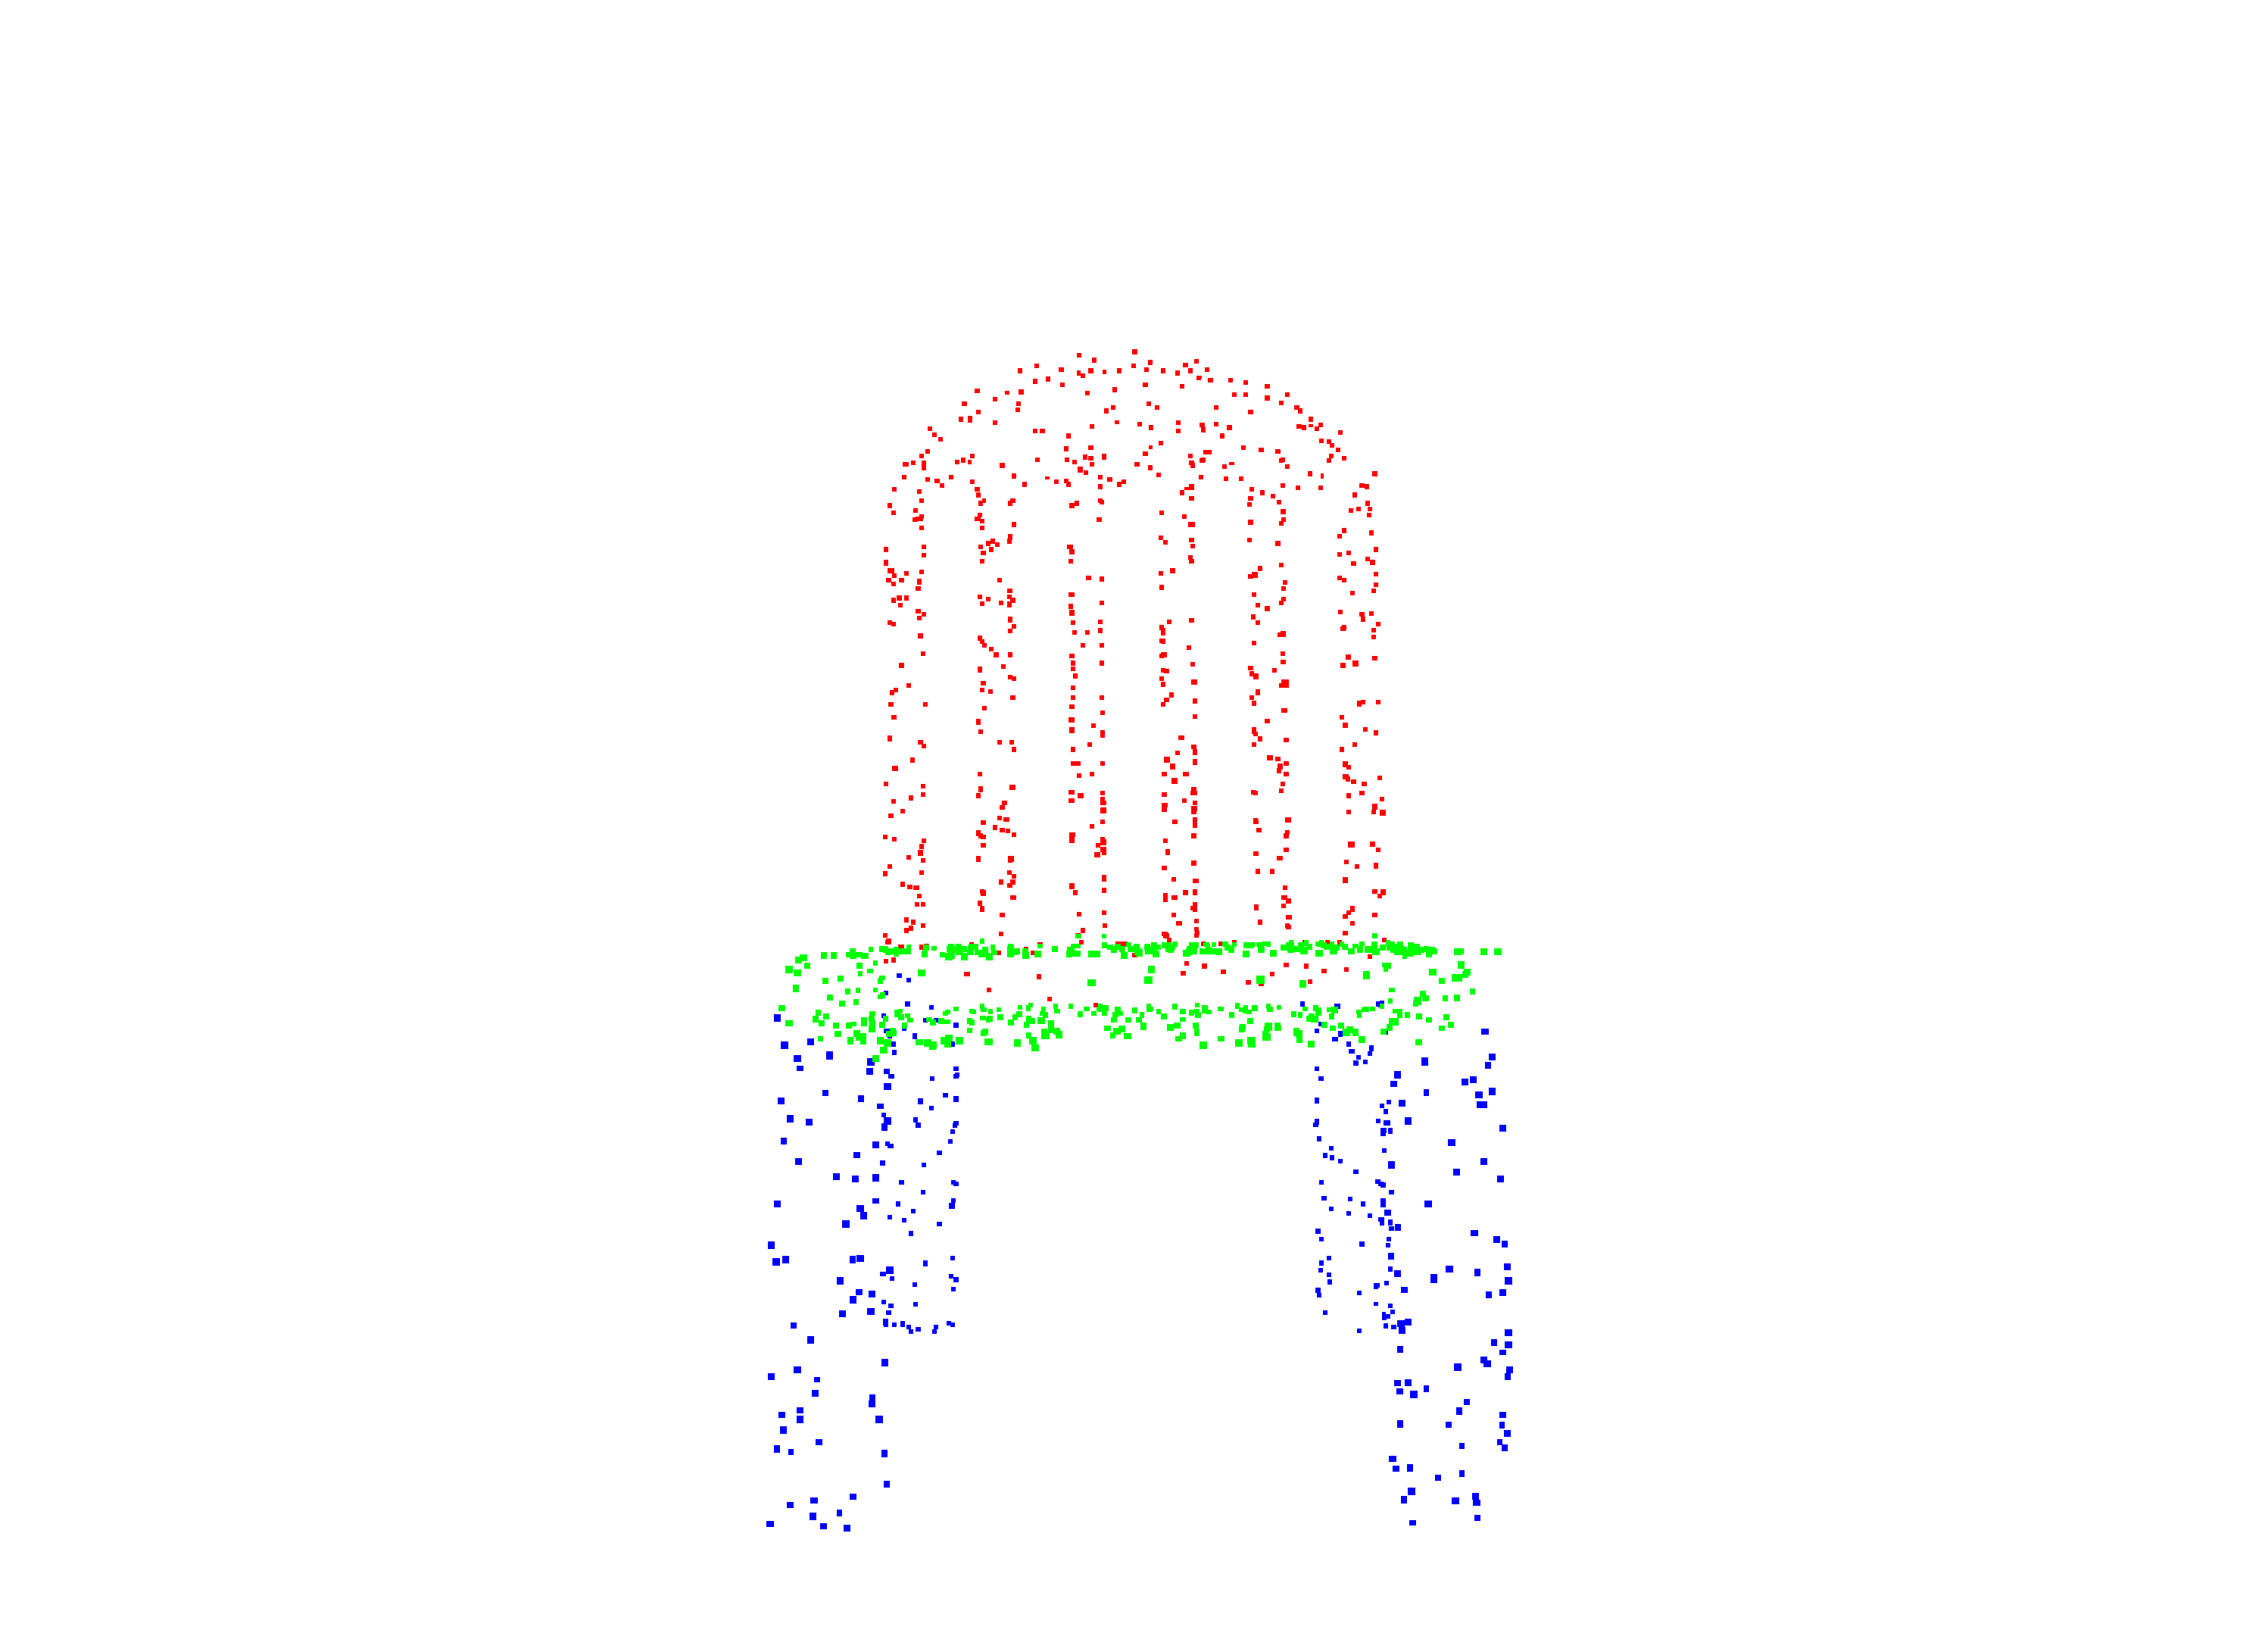
\includegraphics[width=\textwidth]{fig/supplement/part_segmentation/chair/chair01.pdf}
    \end{minipage}
    \hfill
    \begin{minipage}{0.25\textwidth}
        \centering
        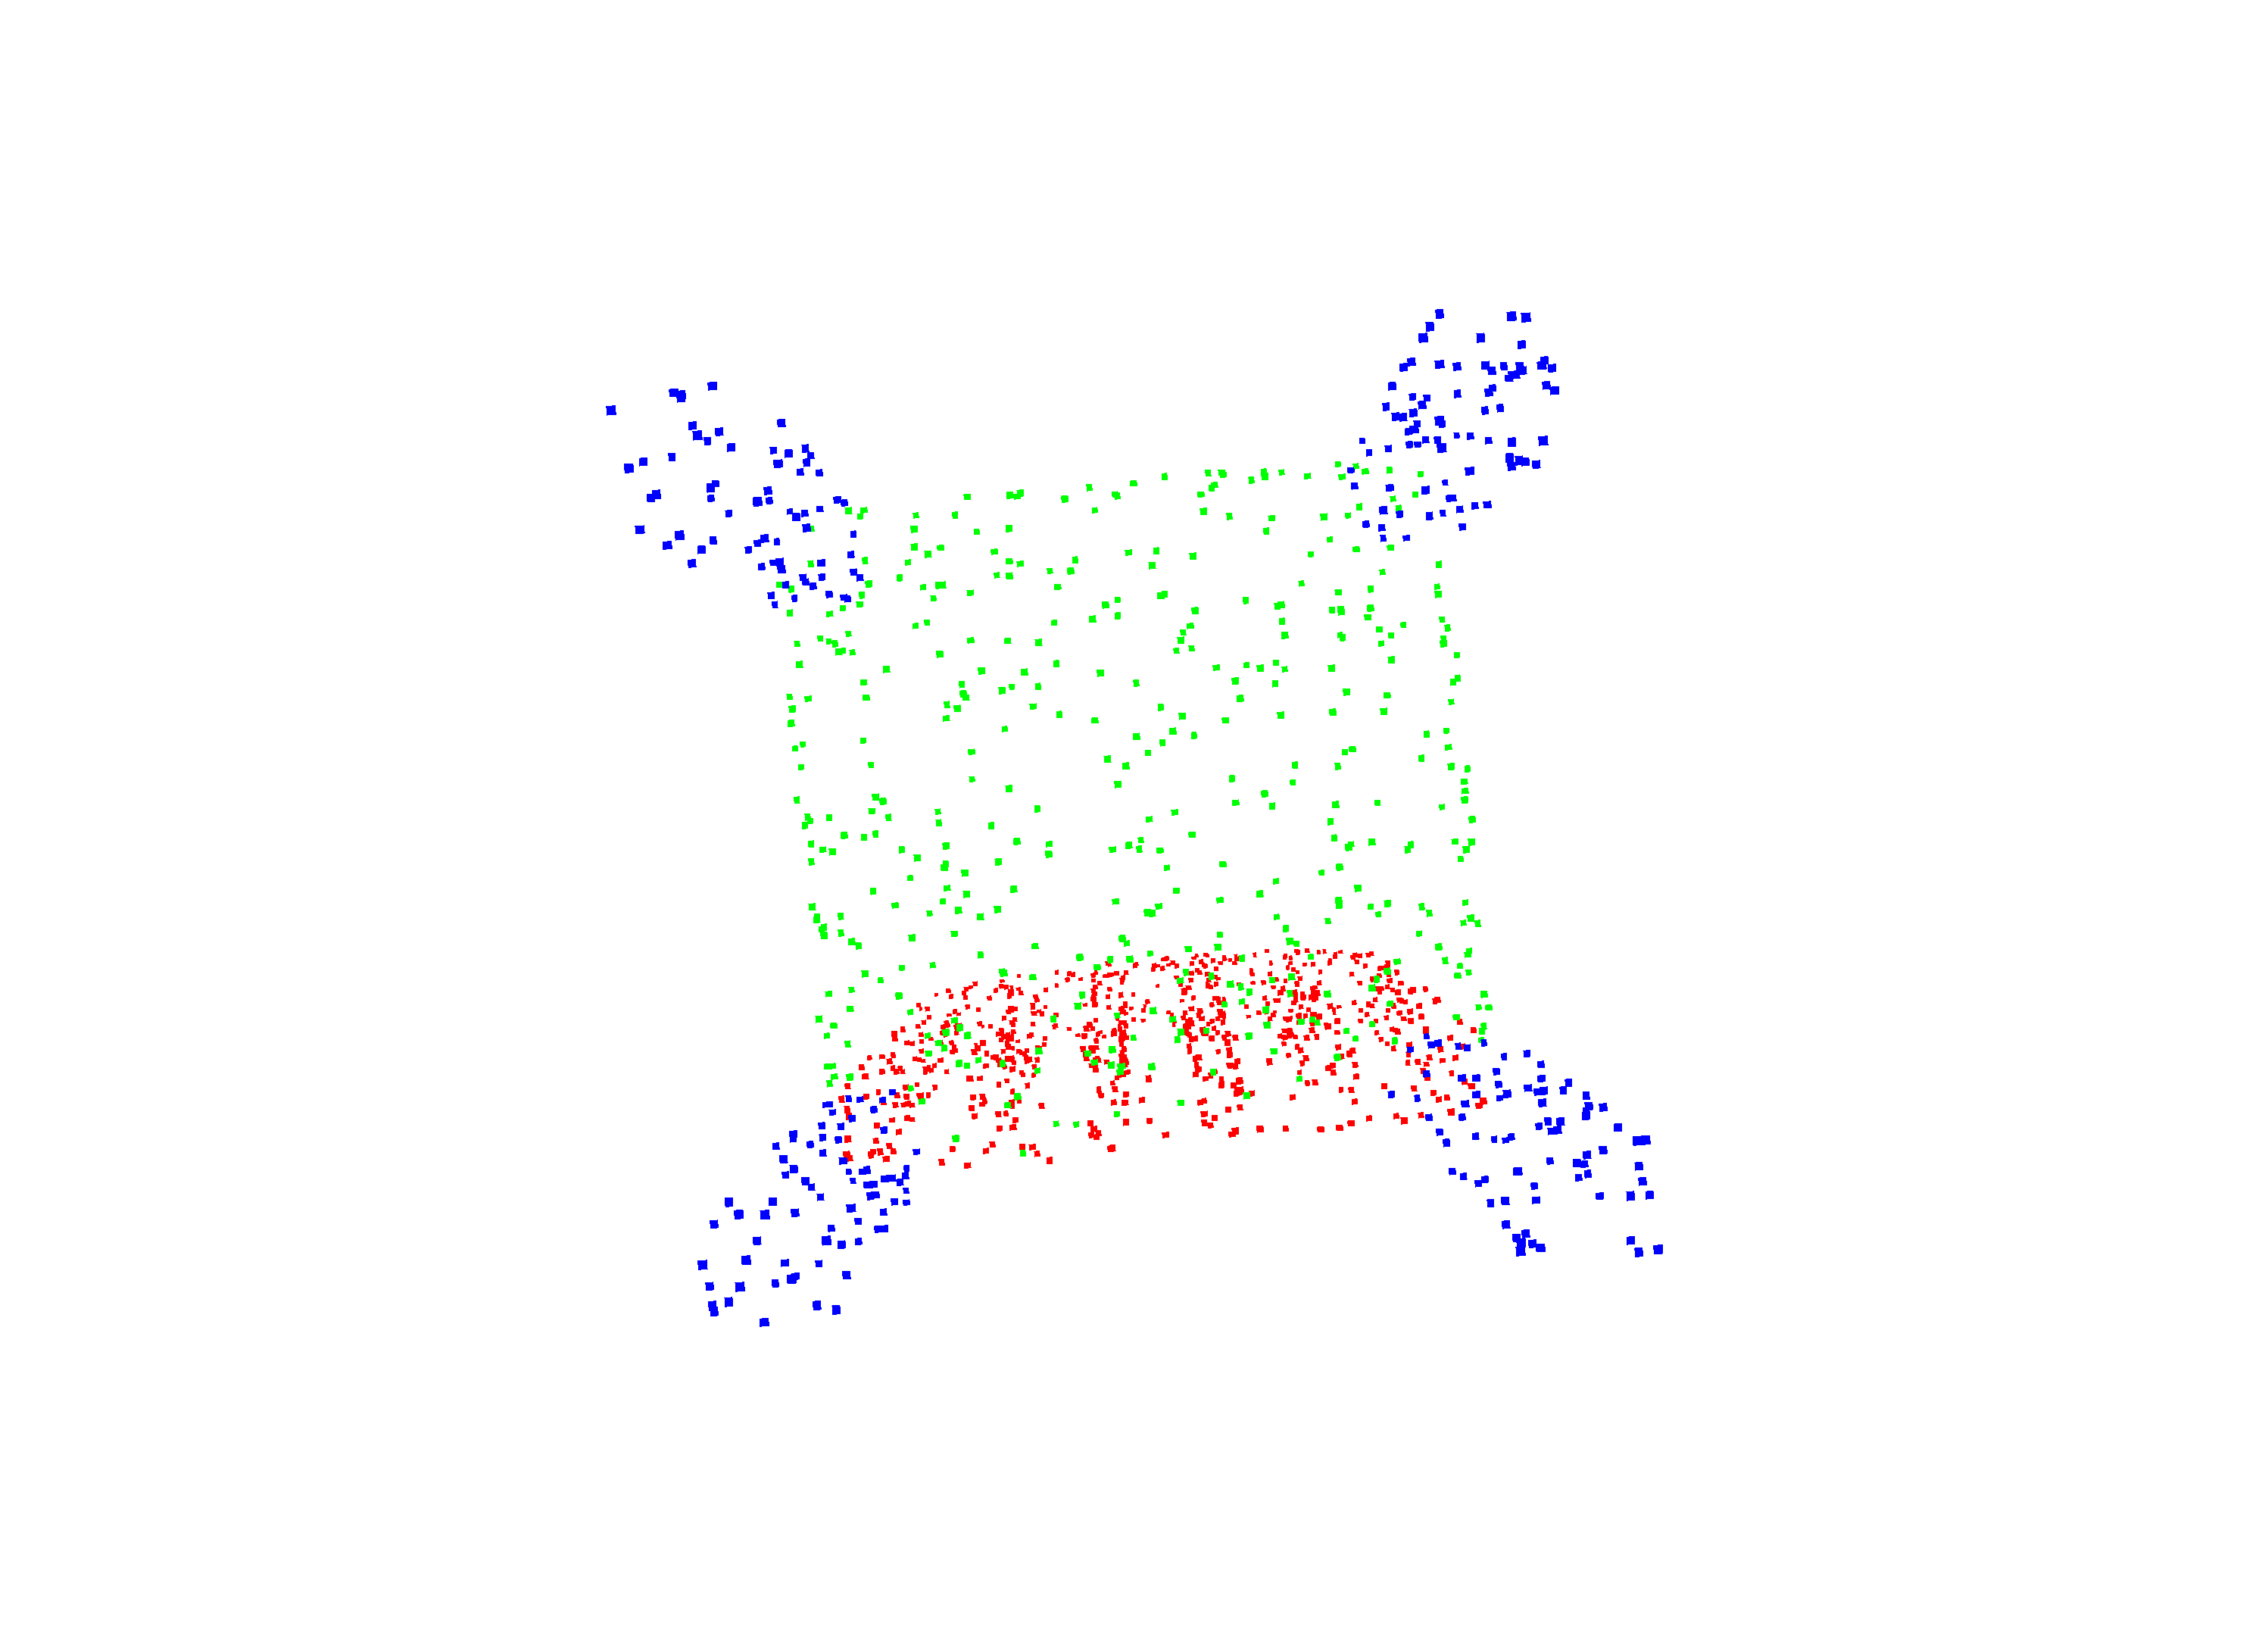
\includegraphics[width=\textwidth]{fig/supplement/part_segmentation/chair/chair02.pdf}
    \end{minipage}
    \hfill

    % 换行
    \vspace{0.5em}

    % 第三行左侧的竖排标签
    \begin{minipage}{0.1\textwidth}
        \centering
        {lamp}
    \end{minipage}
    \hfill
    % 第三行图片
    \begin{minipage}{0.25\textwidth}
        \centering
        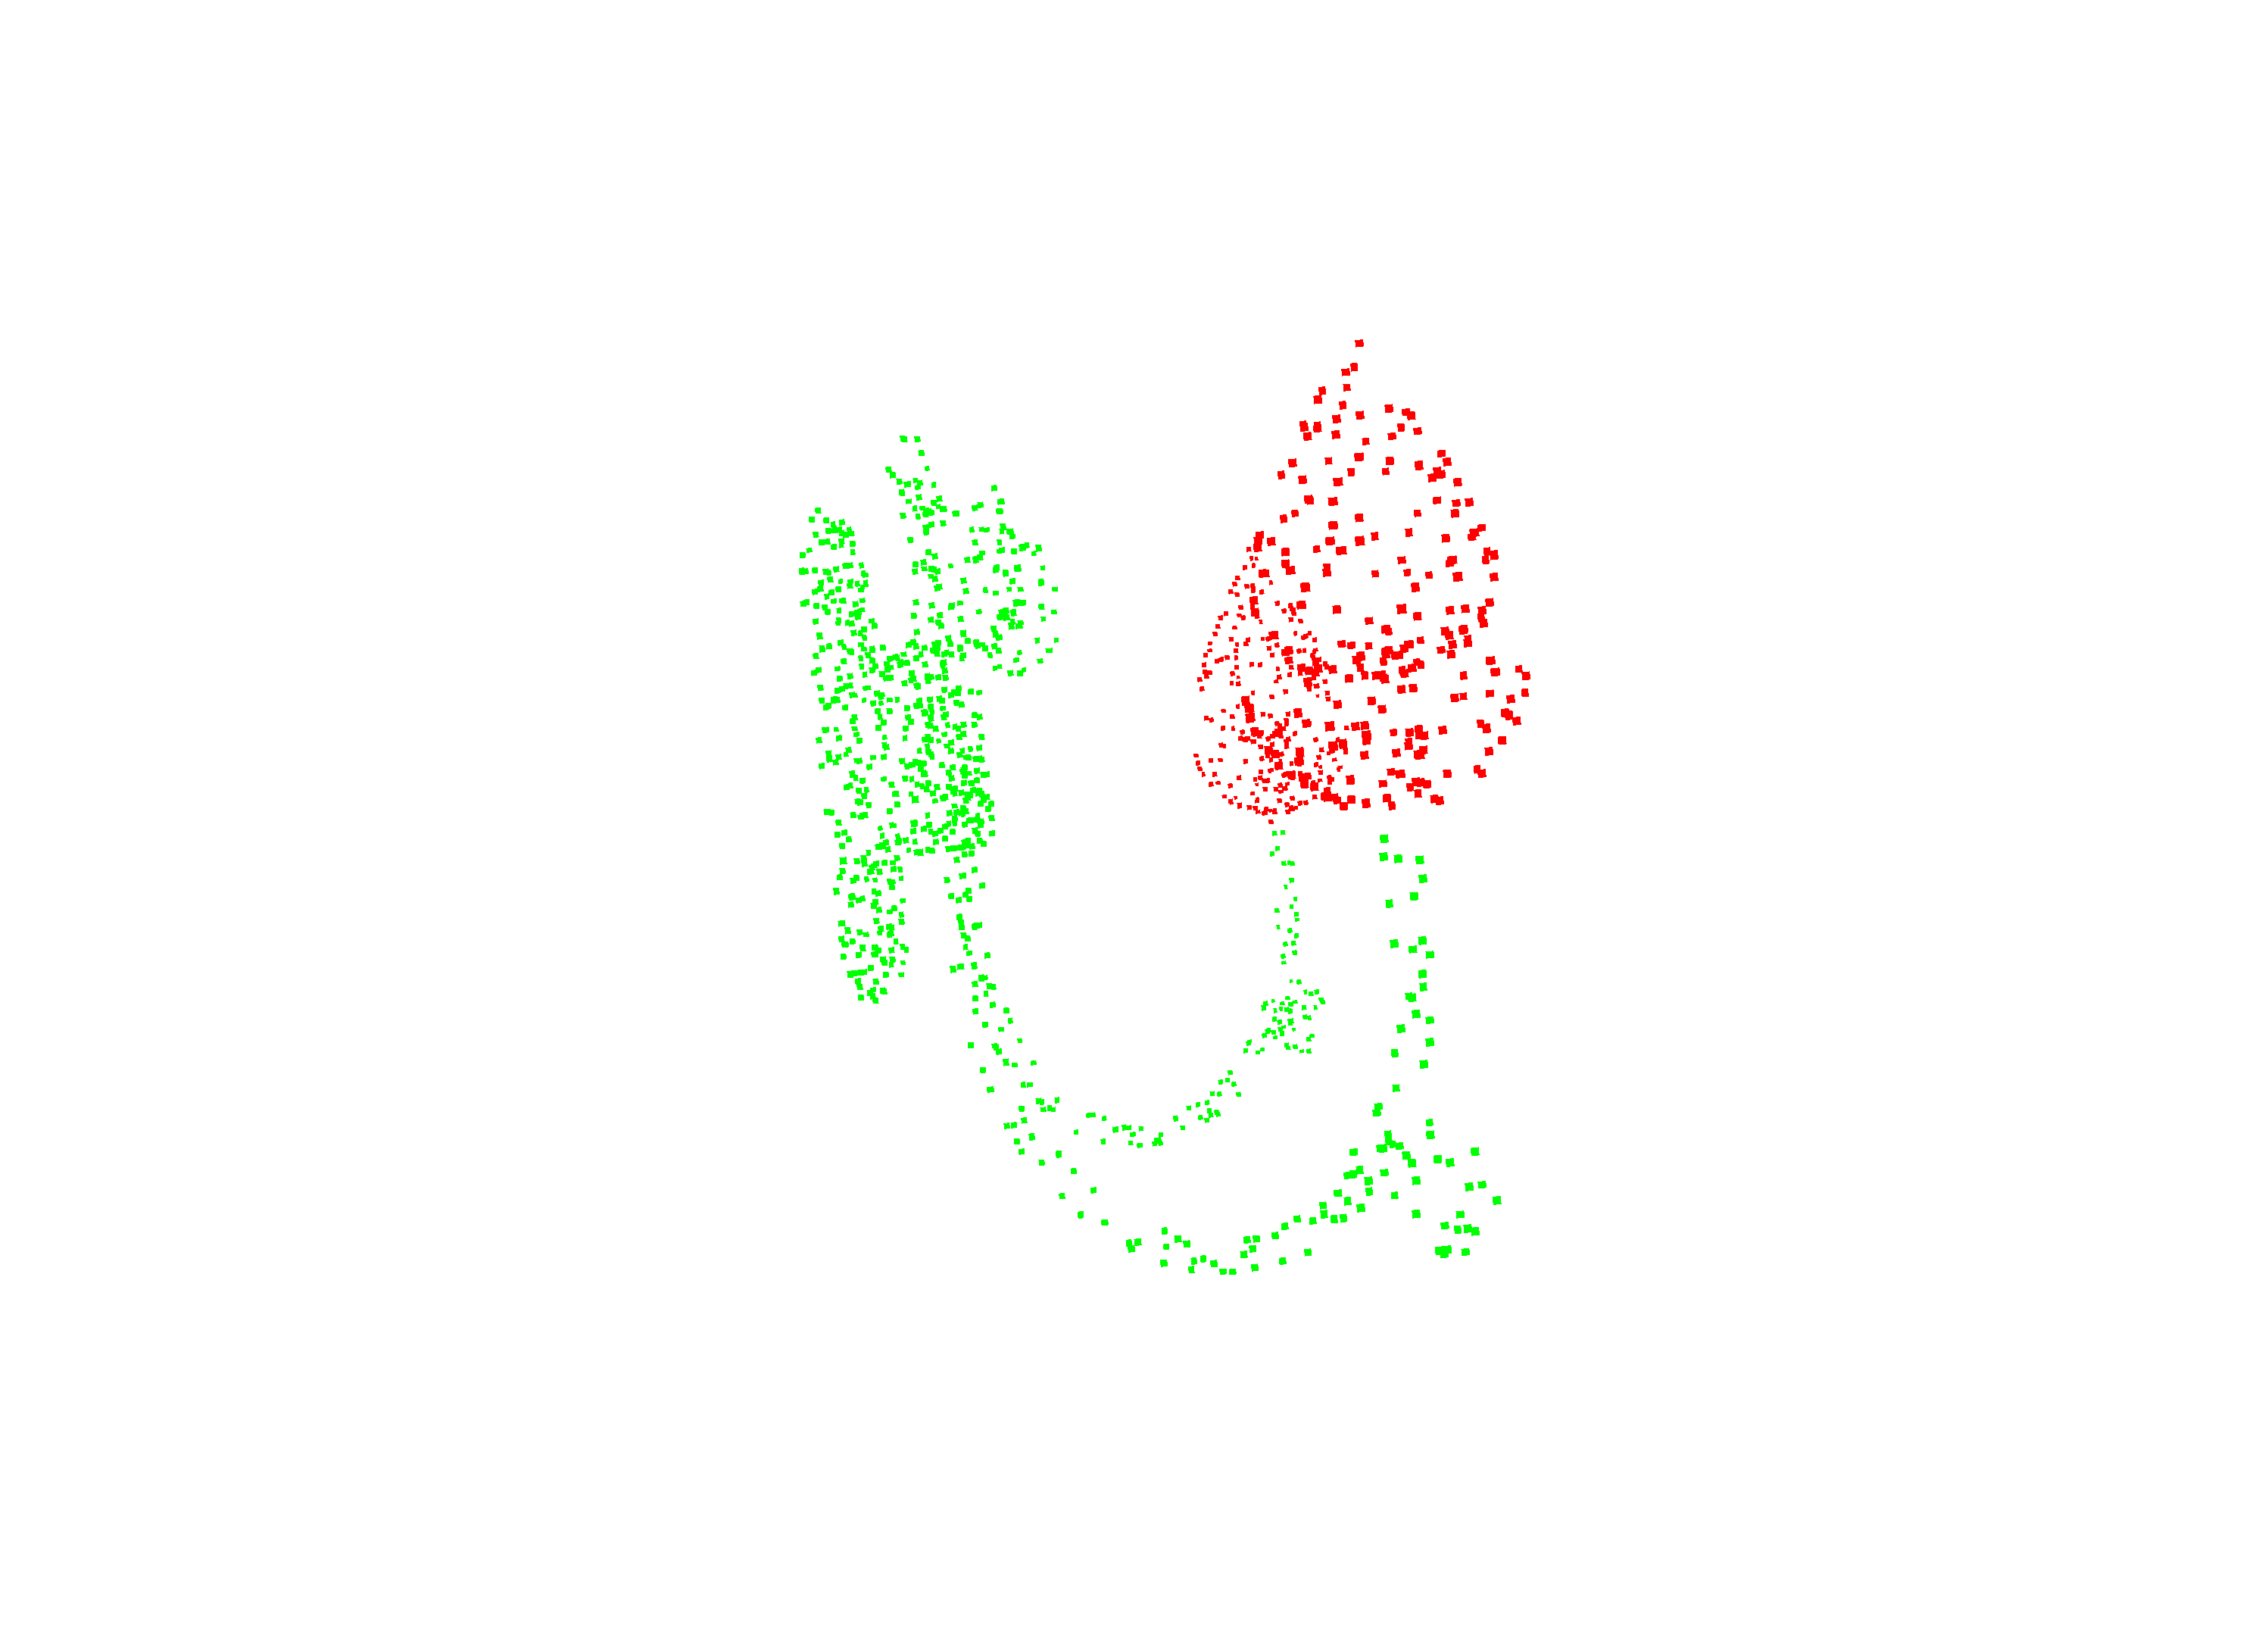
\includegraphics[width=\textwidth]{fig/supplement/part_segmentation/lamp/lamp00.pdf}
    \end{minipage}
    \hfill
    \begin{minipage}{0.25\textwidth}
        \centering
        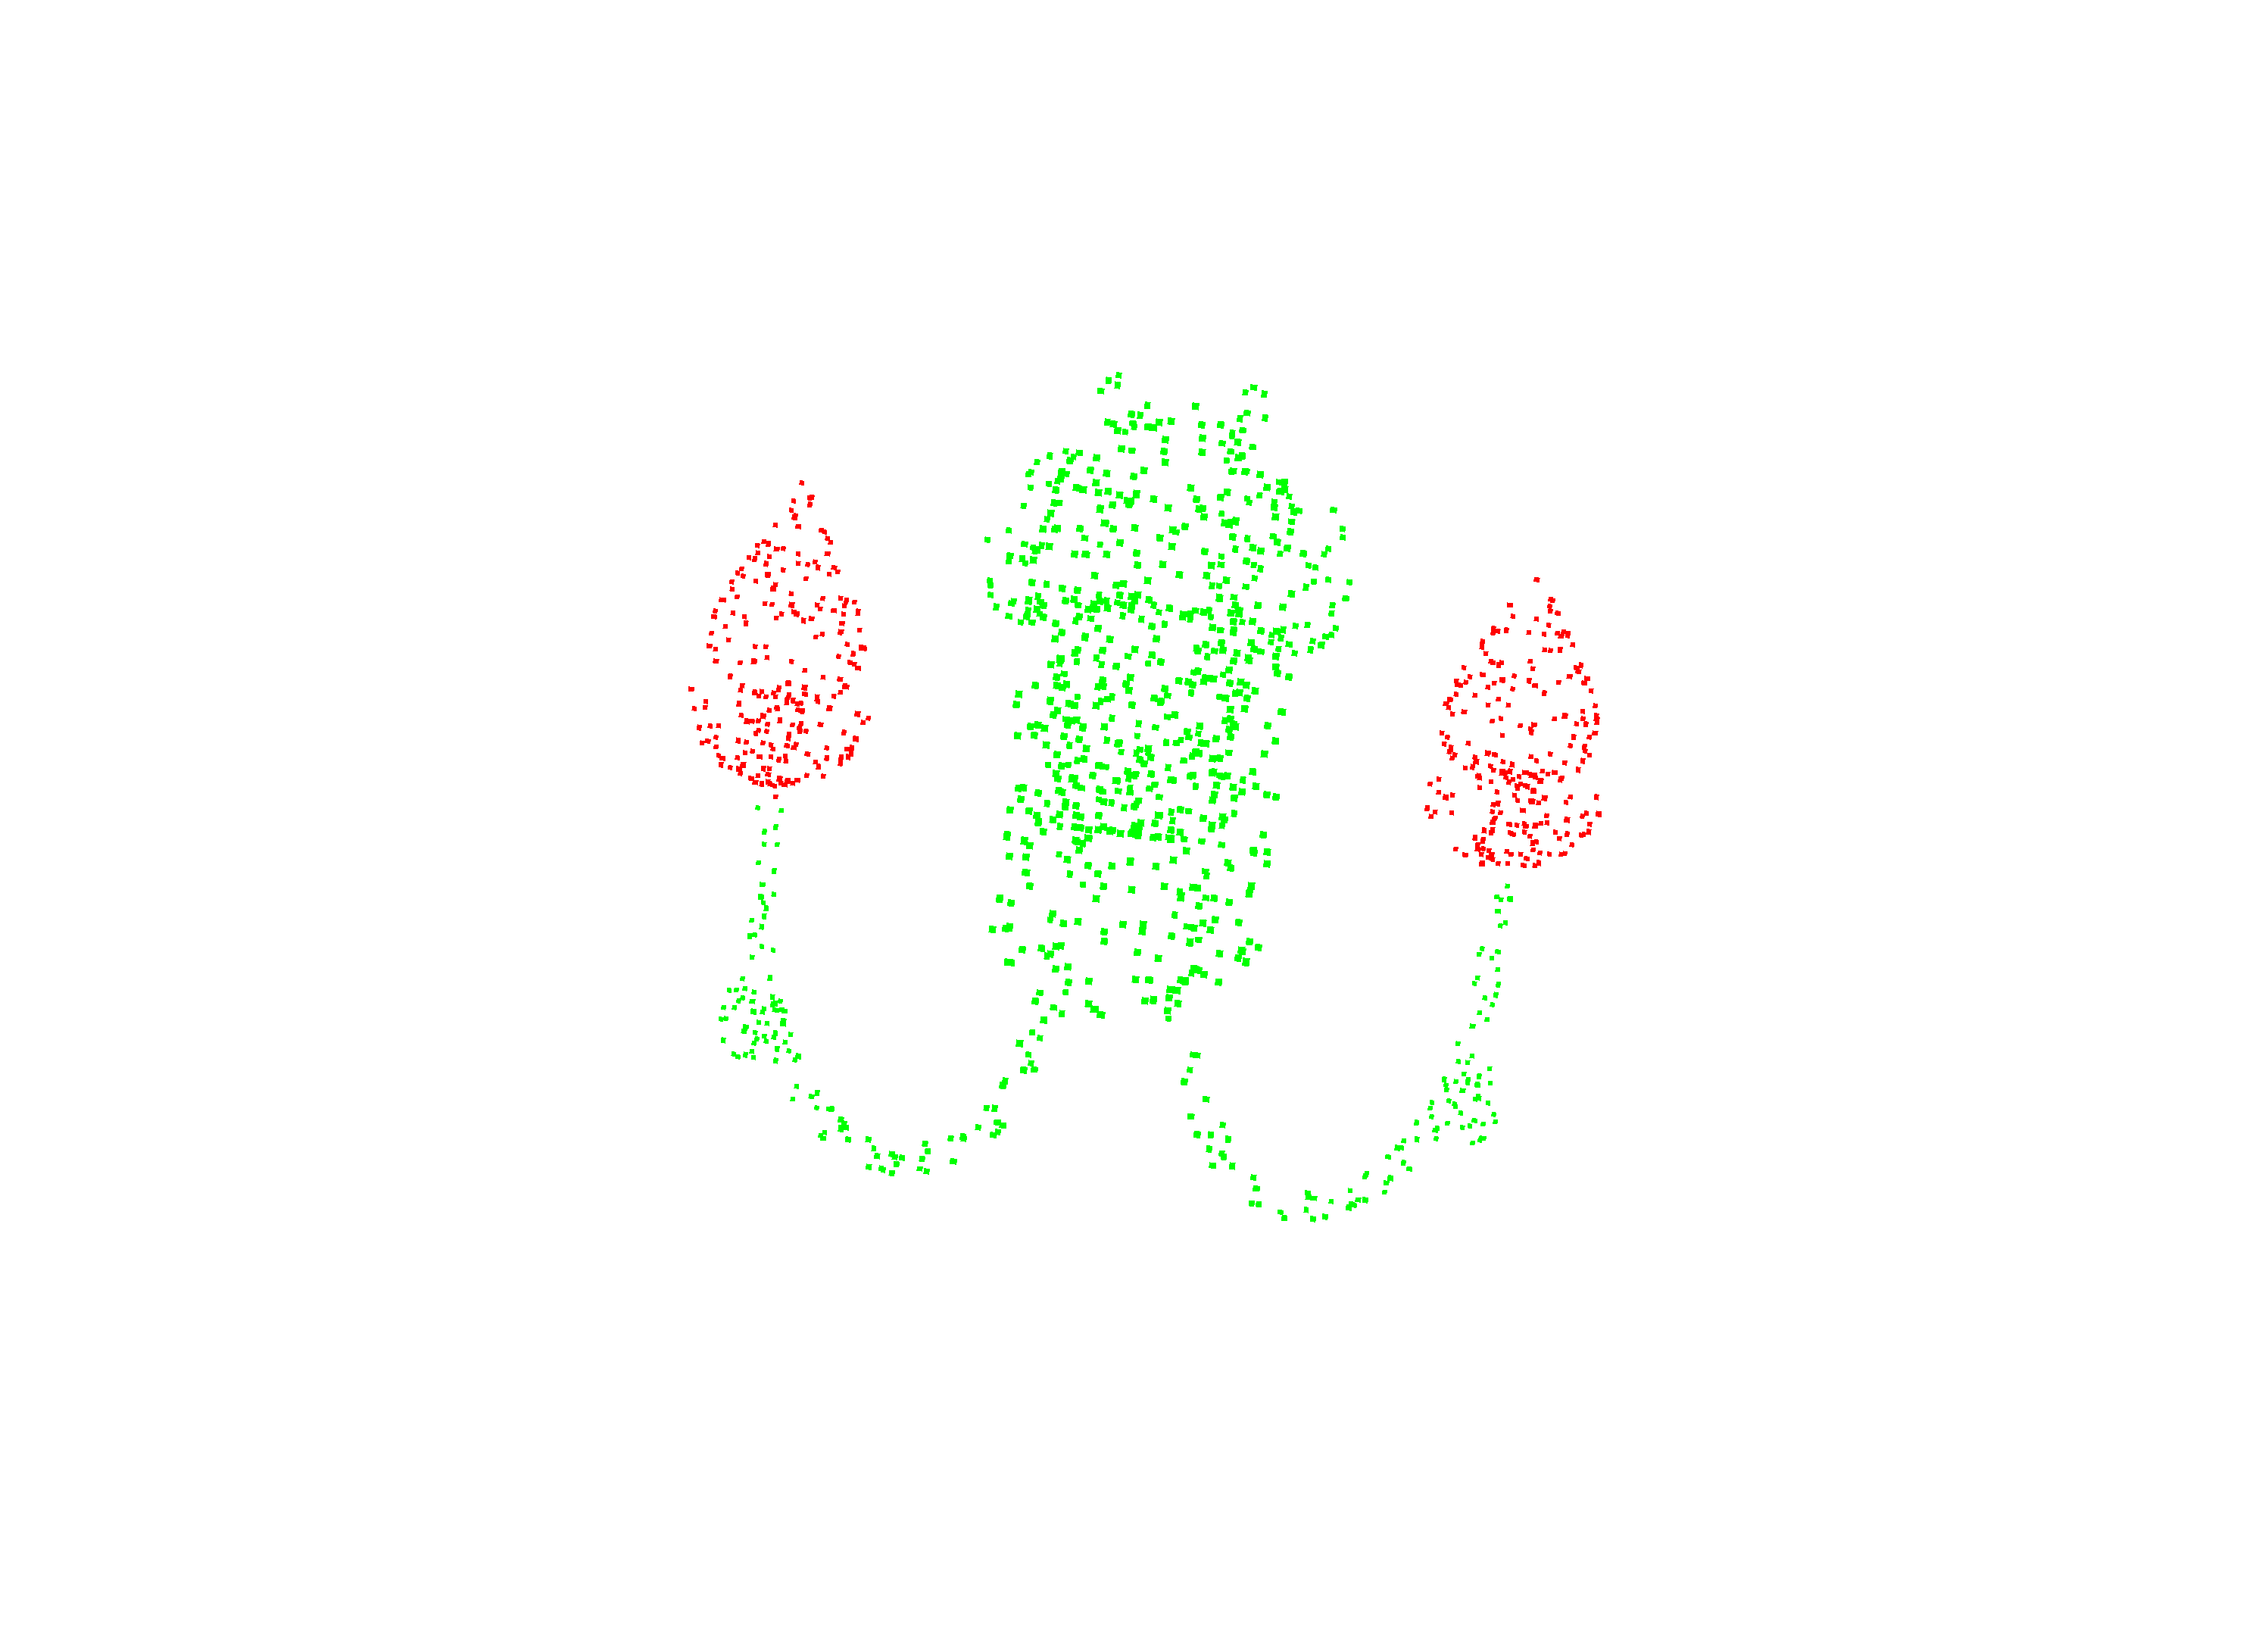
\includegraphics[width=\textwidth]{fig/supplement/part_segmentation/lamp/lamp01.pdf}
    \end{minipage}
    \hfill
    \begin{minipage}{0.25\textwidth}
        \centering
        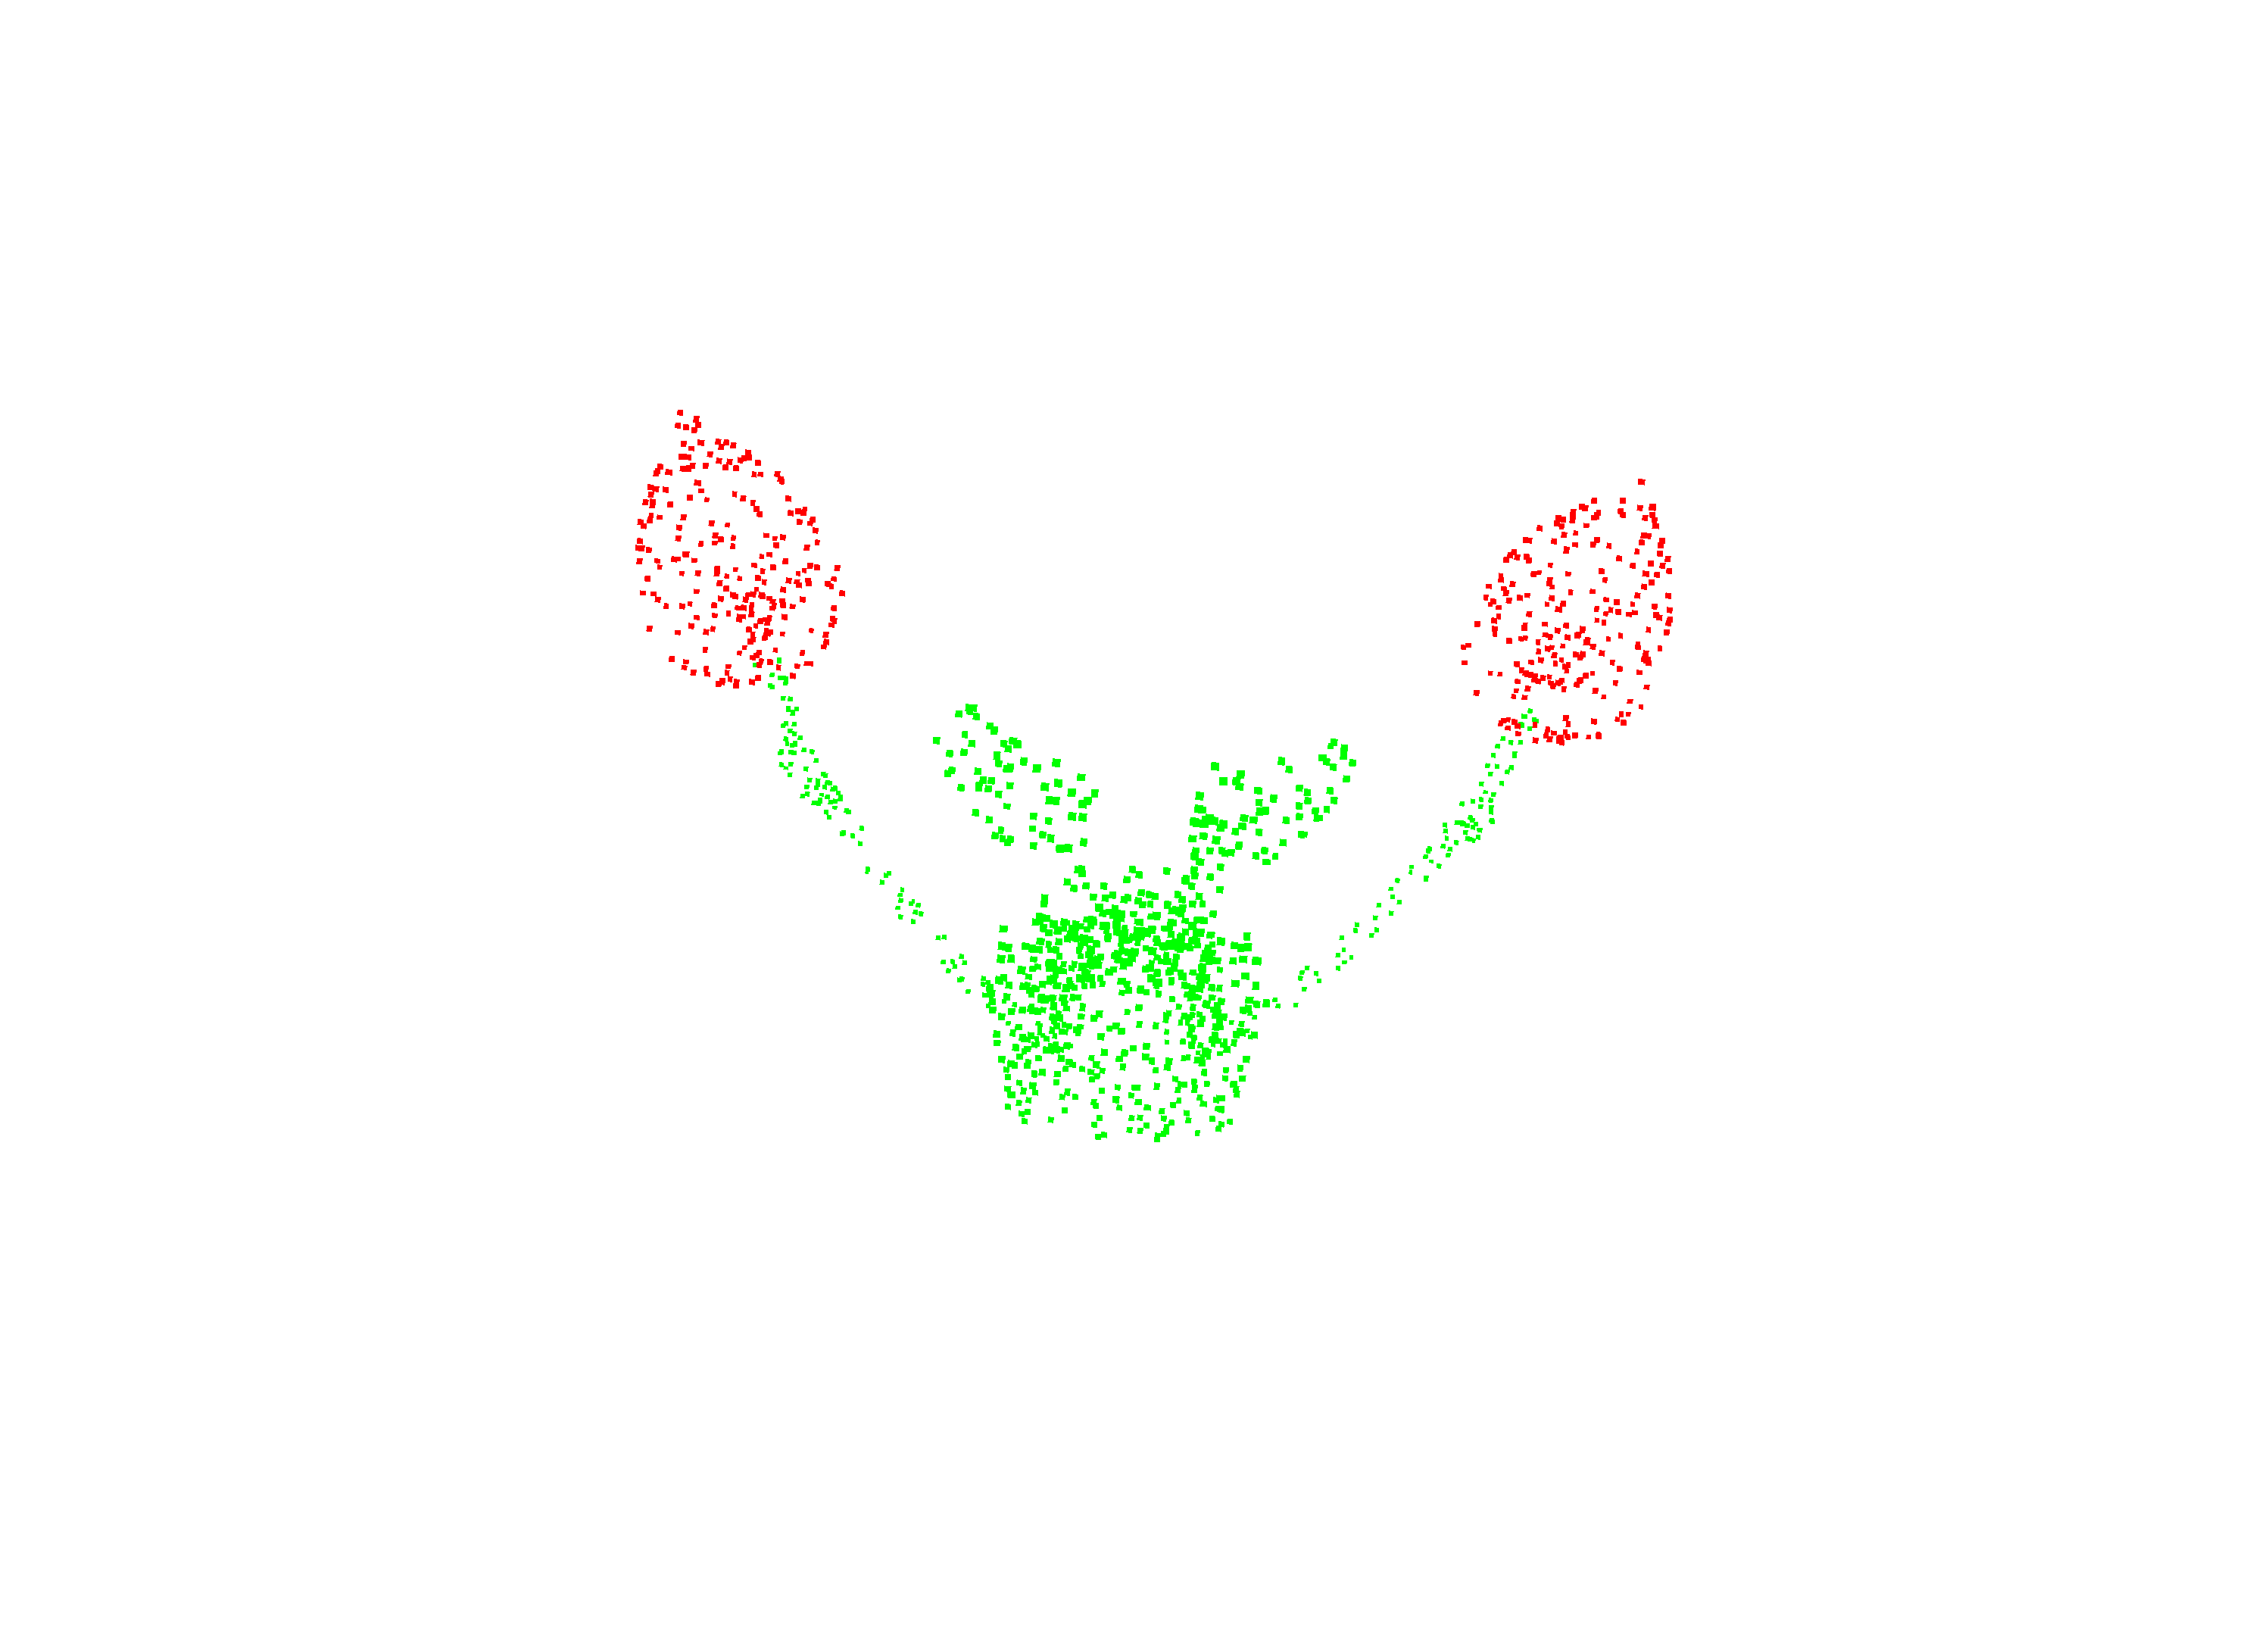
\includegraphics[width=\textwidth]{fig/supplement/part_segmentation/lamp/lamp02.pdf}
    \end{minipage}
    \hfill

    % 换行
    \vspace{0.5em}

    % 第四行左侧的竖排标签
    \begin{minipage}{0.1\textwidth}
        \centering
        {skateboard}
    \end{minipage}
    \hfill
    % 第四行图片
    \begin{minipage}{0.25\textwidth}
        \centering
        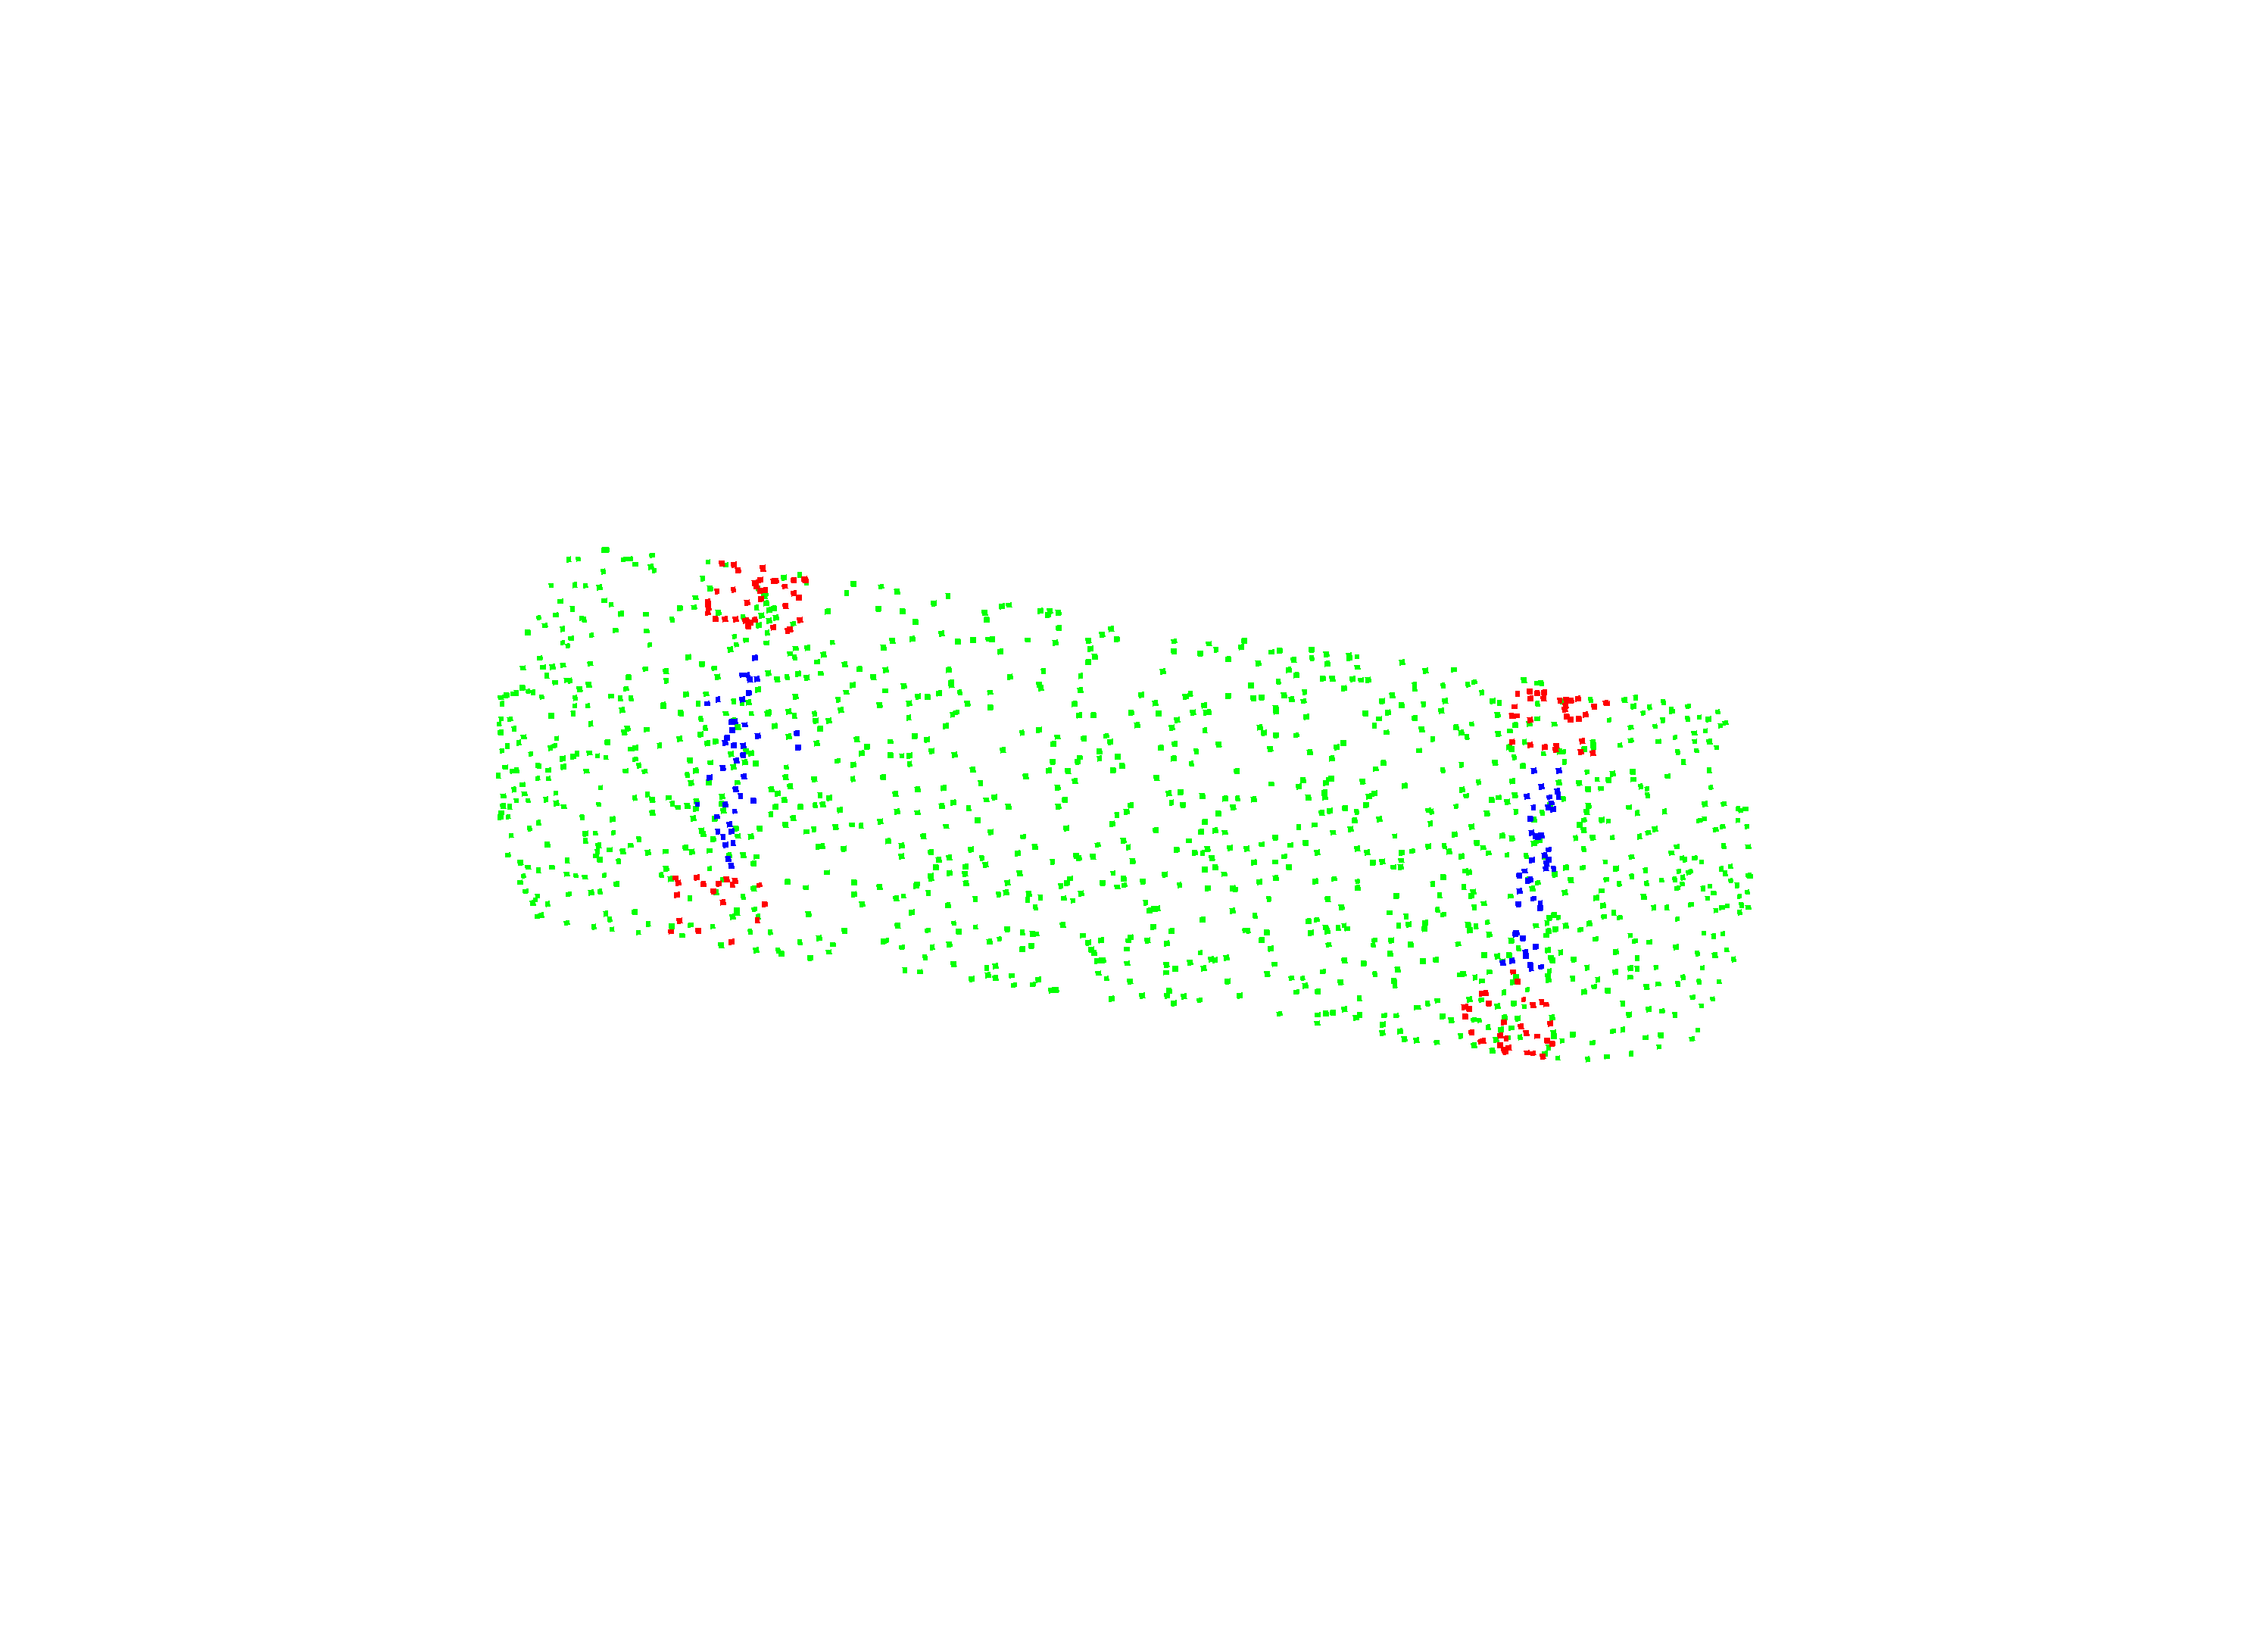
\includegraphics[width=\textwidth]{fig/supplement/part_segmentation/skateboard/skateboard00.pdf}
    \end{minipage}
    \hfill
    \begin{minipage}{0.25\textwidth}
        \centering
        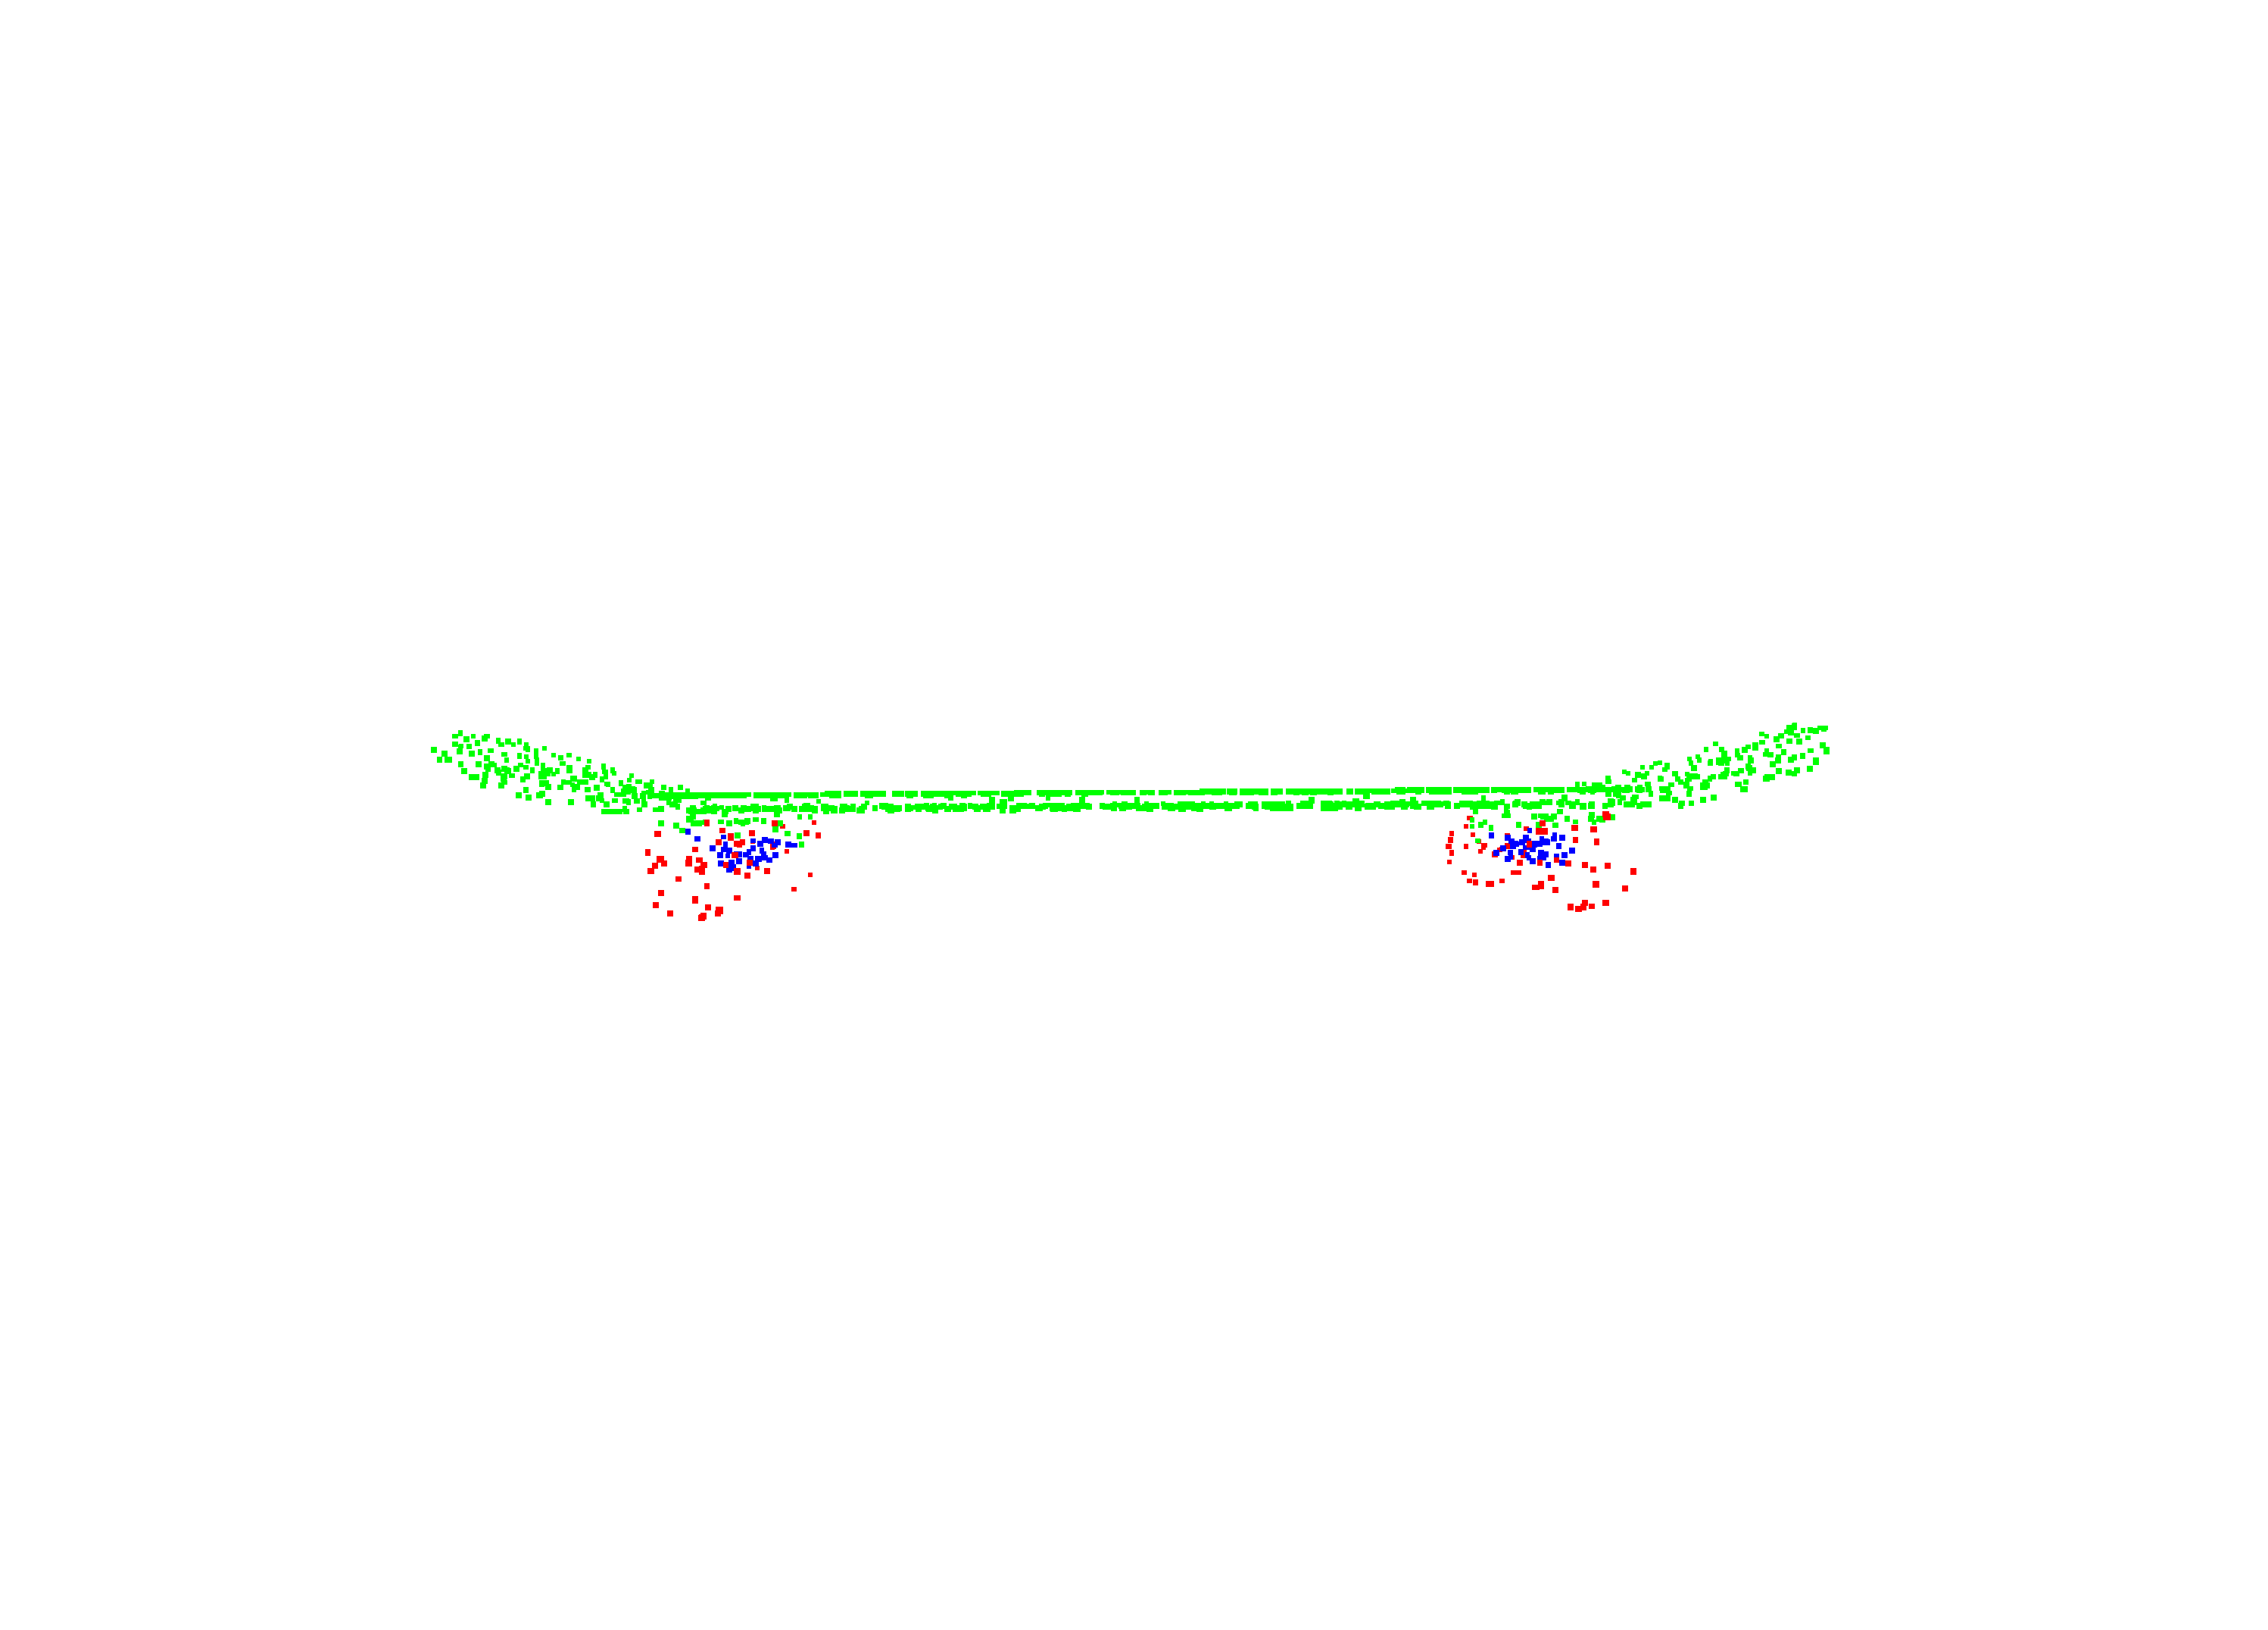
\includegraphics[width=\textwidth]{fig/supplement/part_segmentation/skateboard/skateboard01.pdf}
    \end{minipage}
    \hfill
    \begin{minipage}{0.25\textwidth}
        \centering
        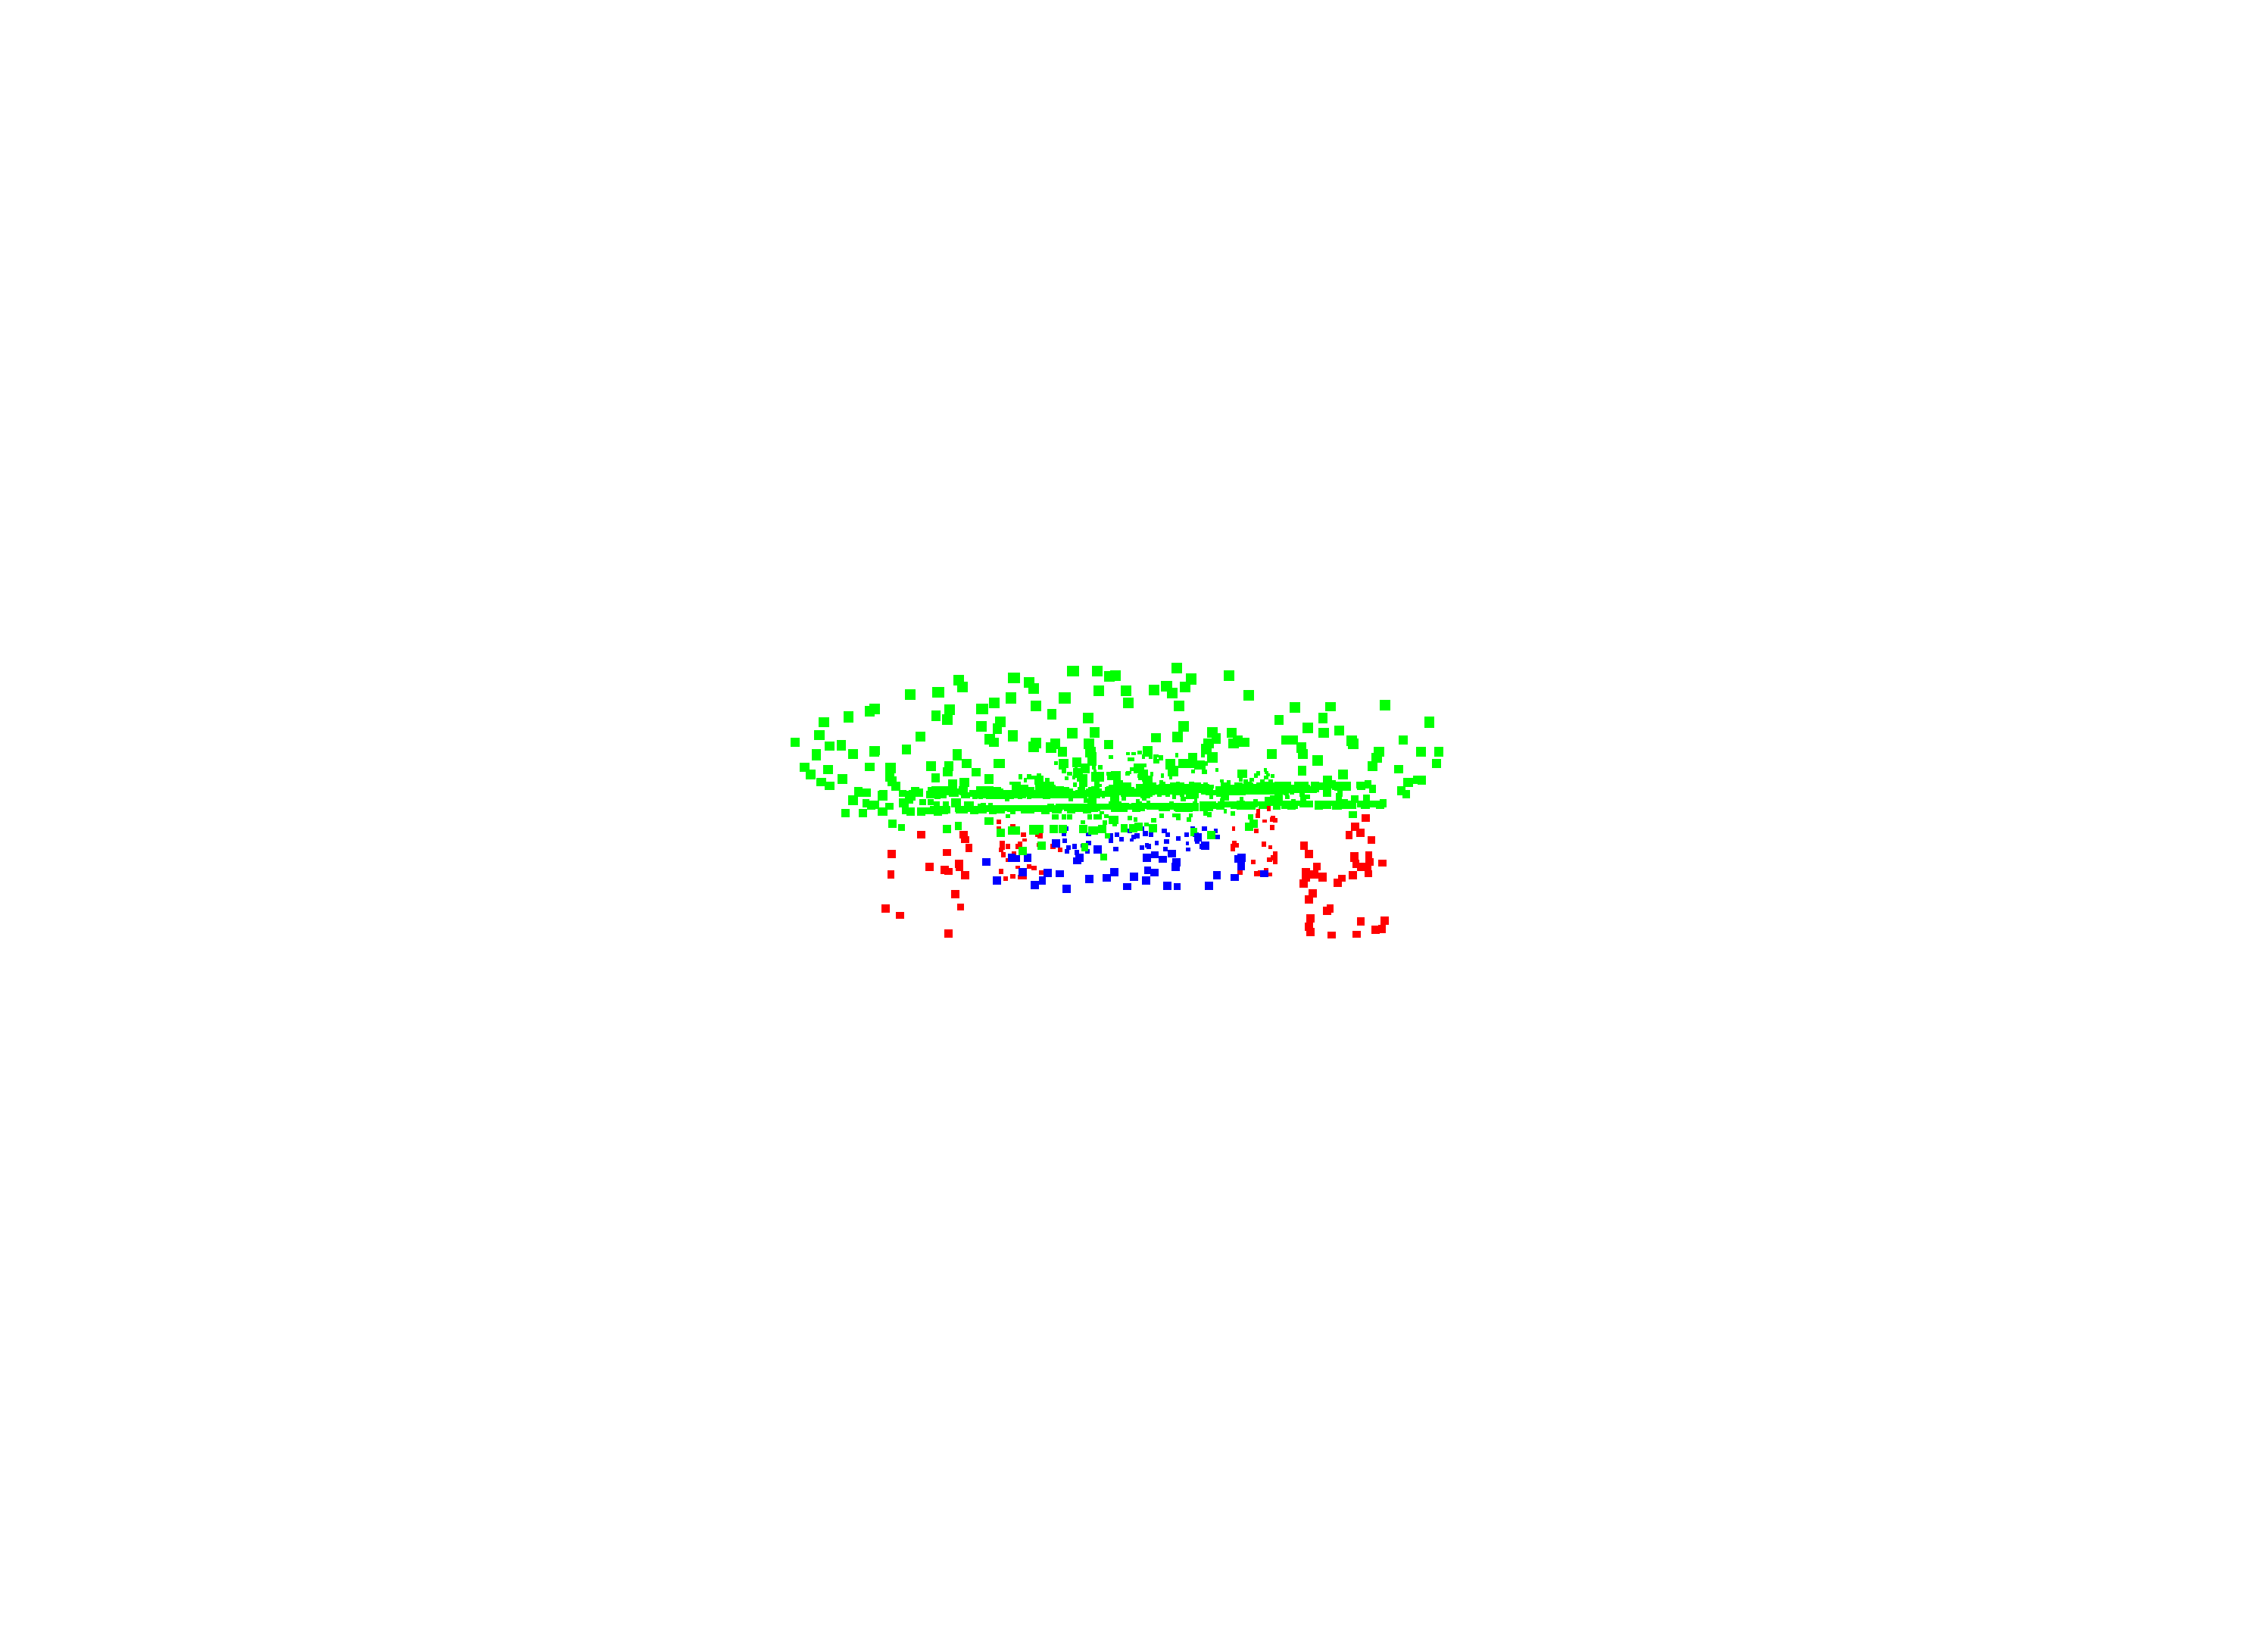
\includegraphics[width=\textwidth]{fig/supplement/part_segmentation/skateboard/skateboard02.pdf}
    \end{minipage}
    \hfill

    % 换行
    \vspace{0.5em}

    % 第五行左侧的竖排标签
    \begin{minipage}{0.1\textwidth}
        \centering
        {table}
    \end{minipage}
    \hfill
    % 第五行图片
    \begin{minipage}{0.25\textwidth}
        \centering
        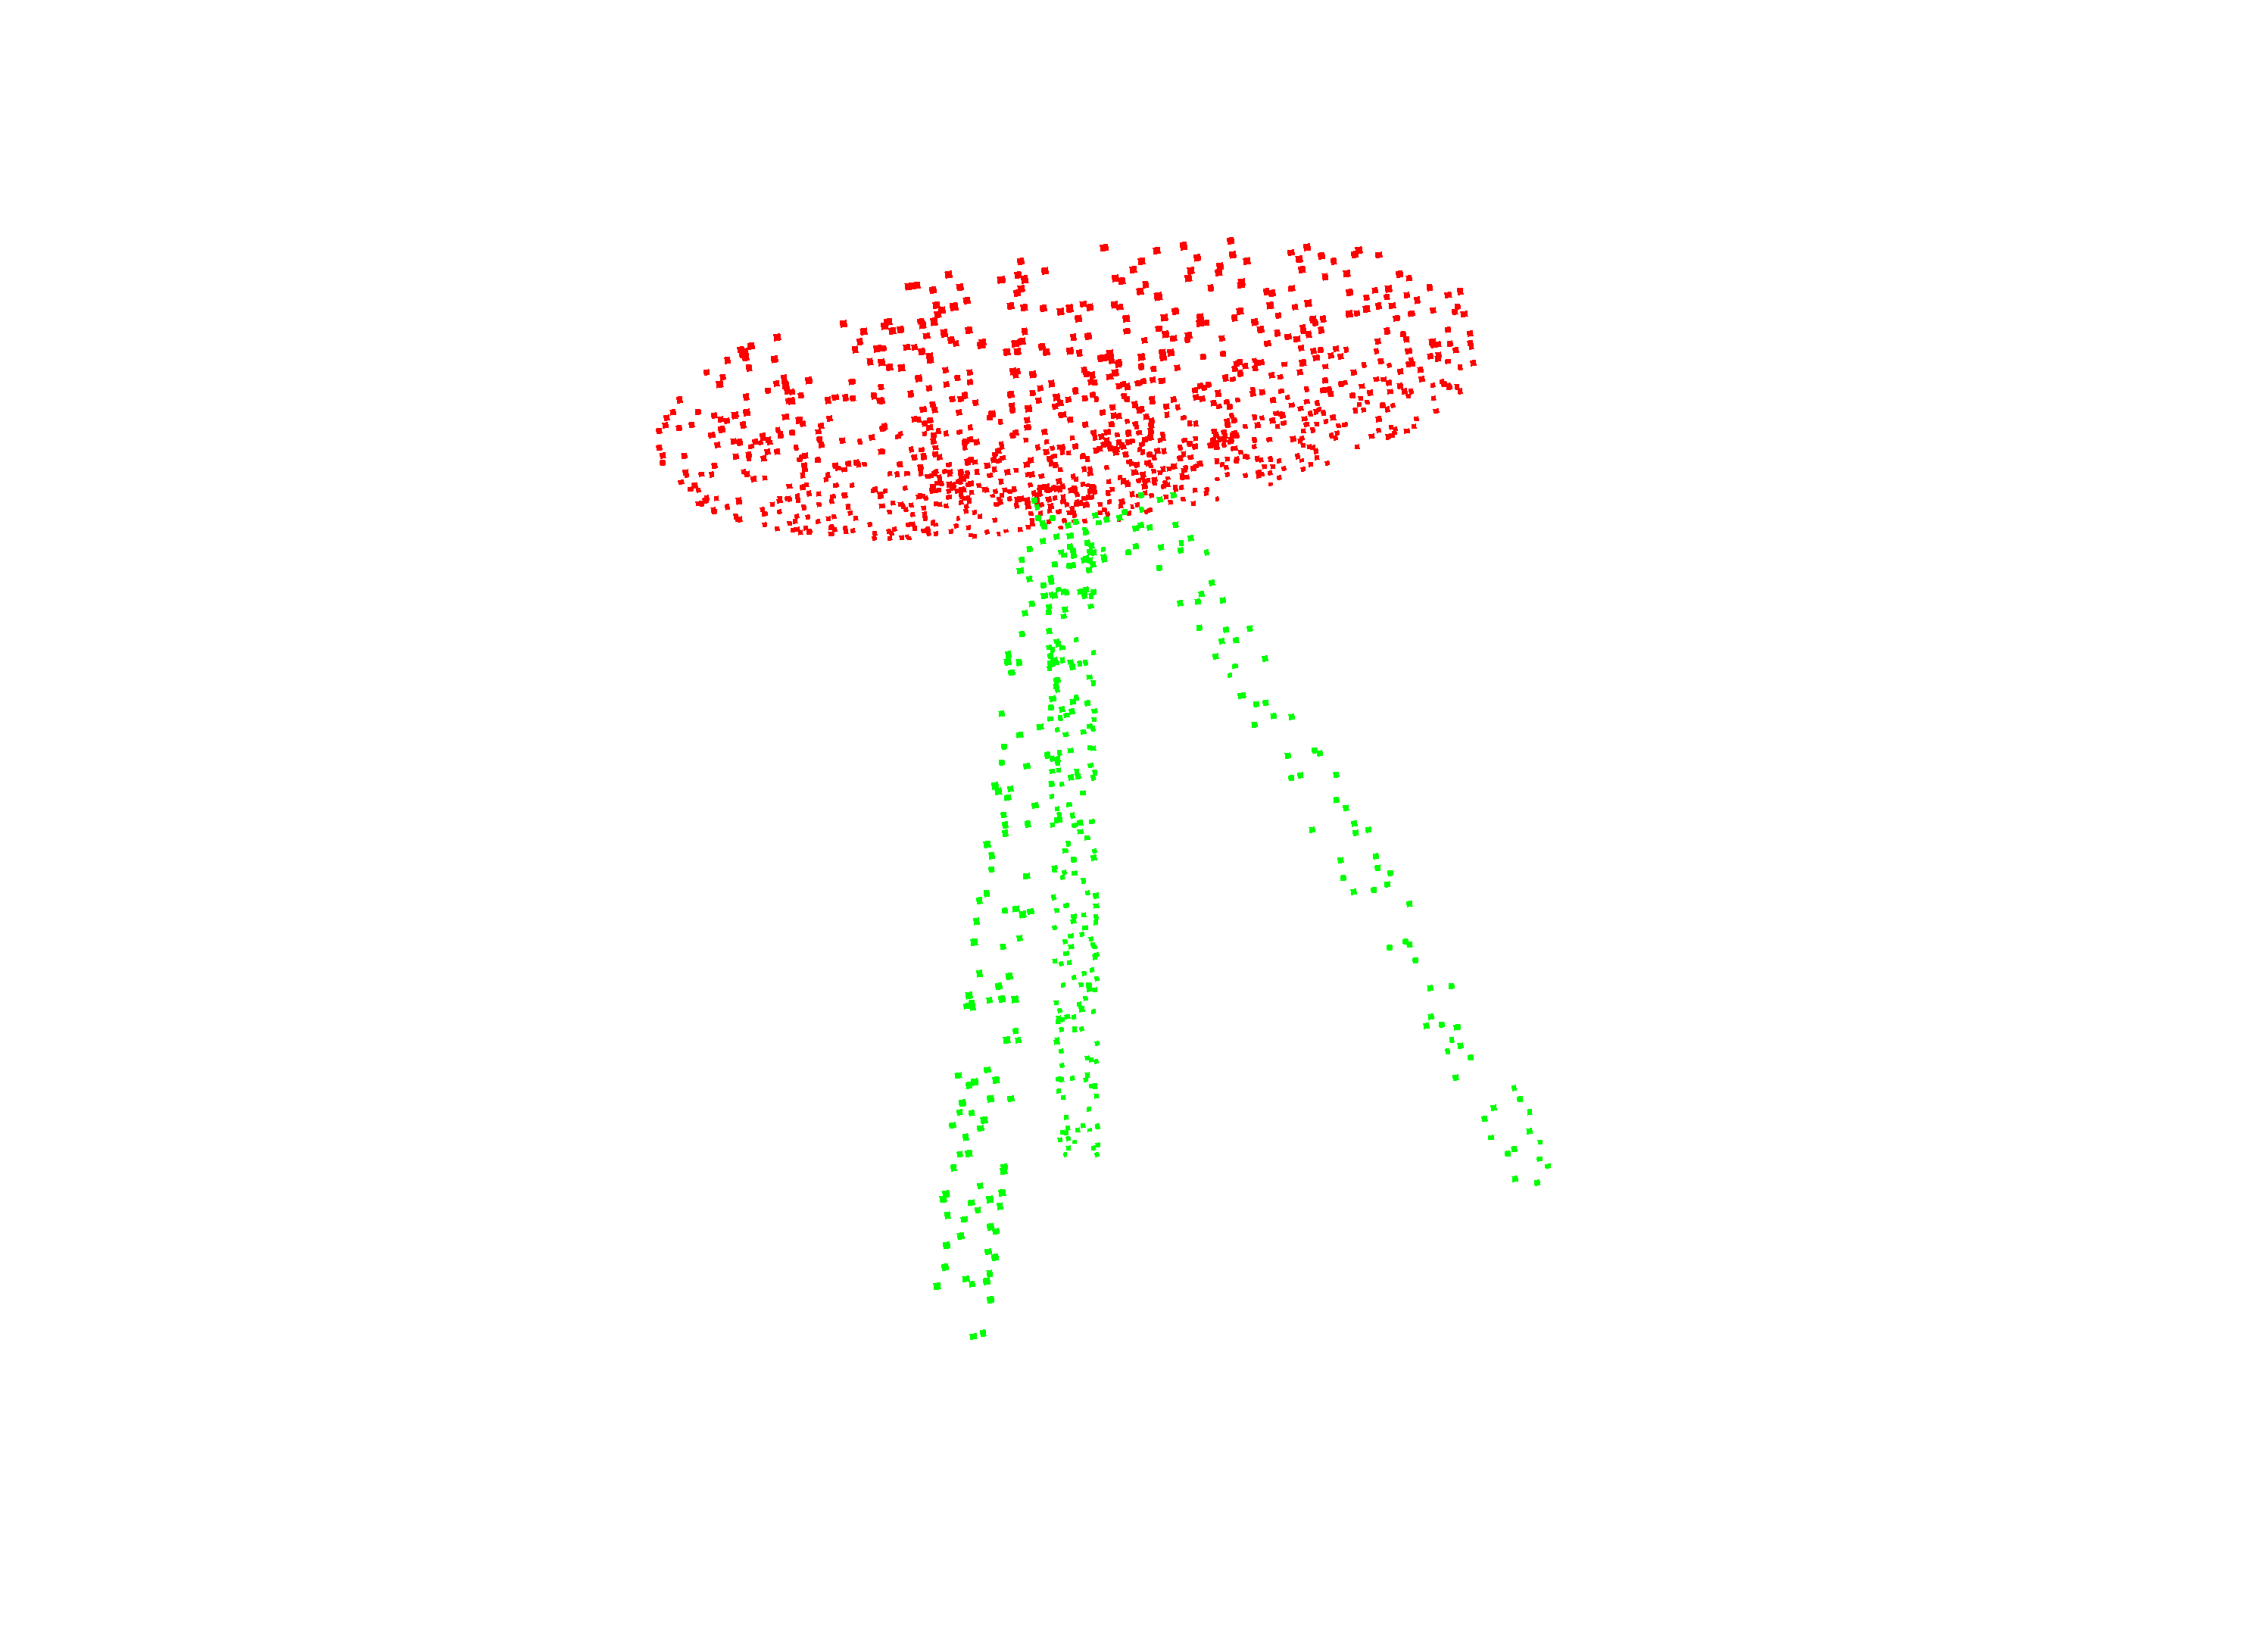
\includegraphics[width=\textwidth]{fig/supplement/part_segmentation/table/table00.pdf}
    \end{minipage}
    \hfill
    \begin{minipage}{0.25\textwidth}
        \centering
        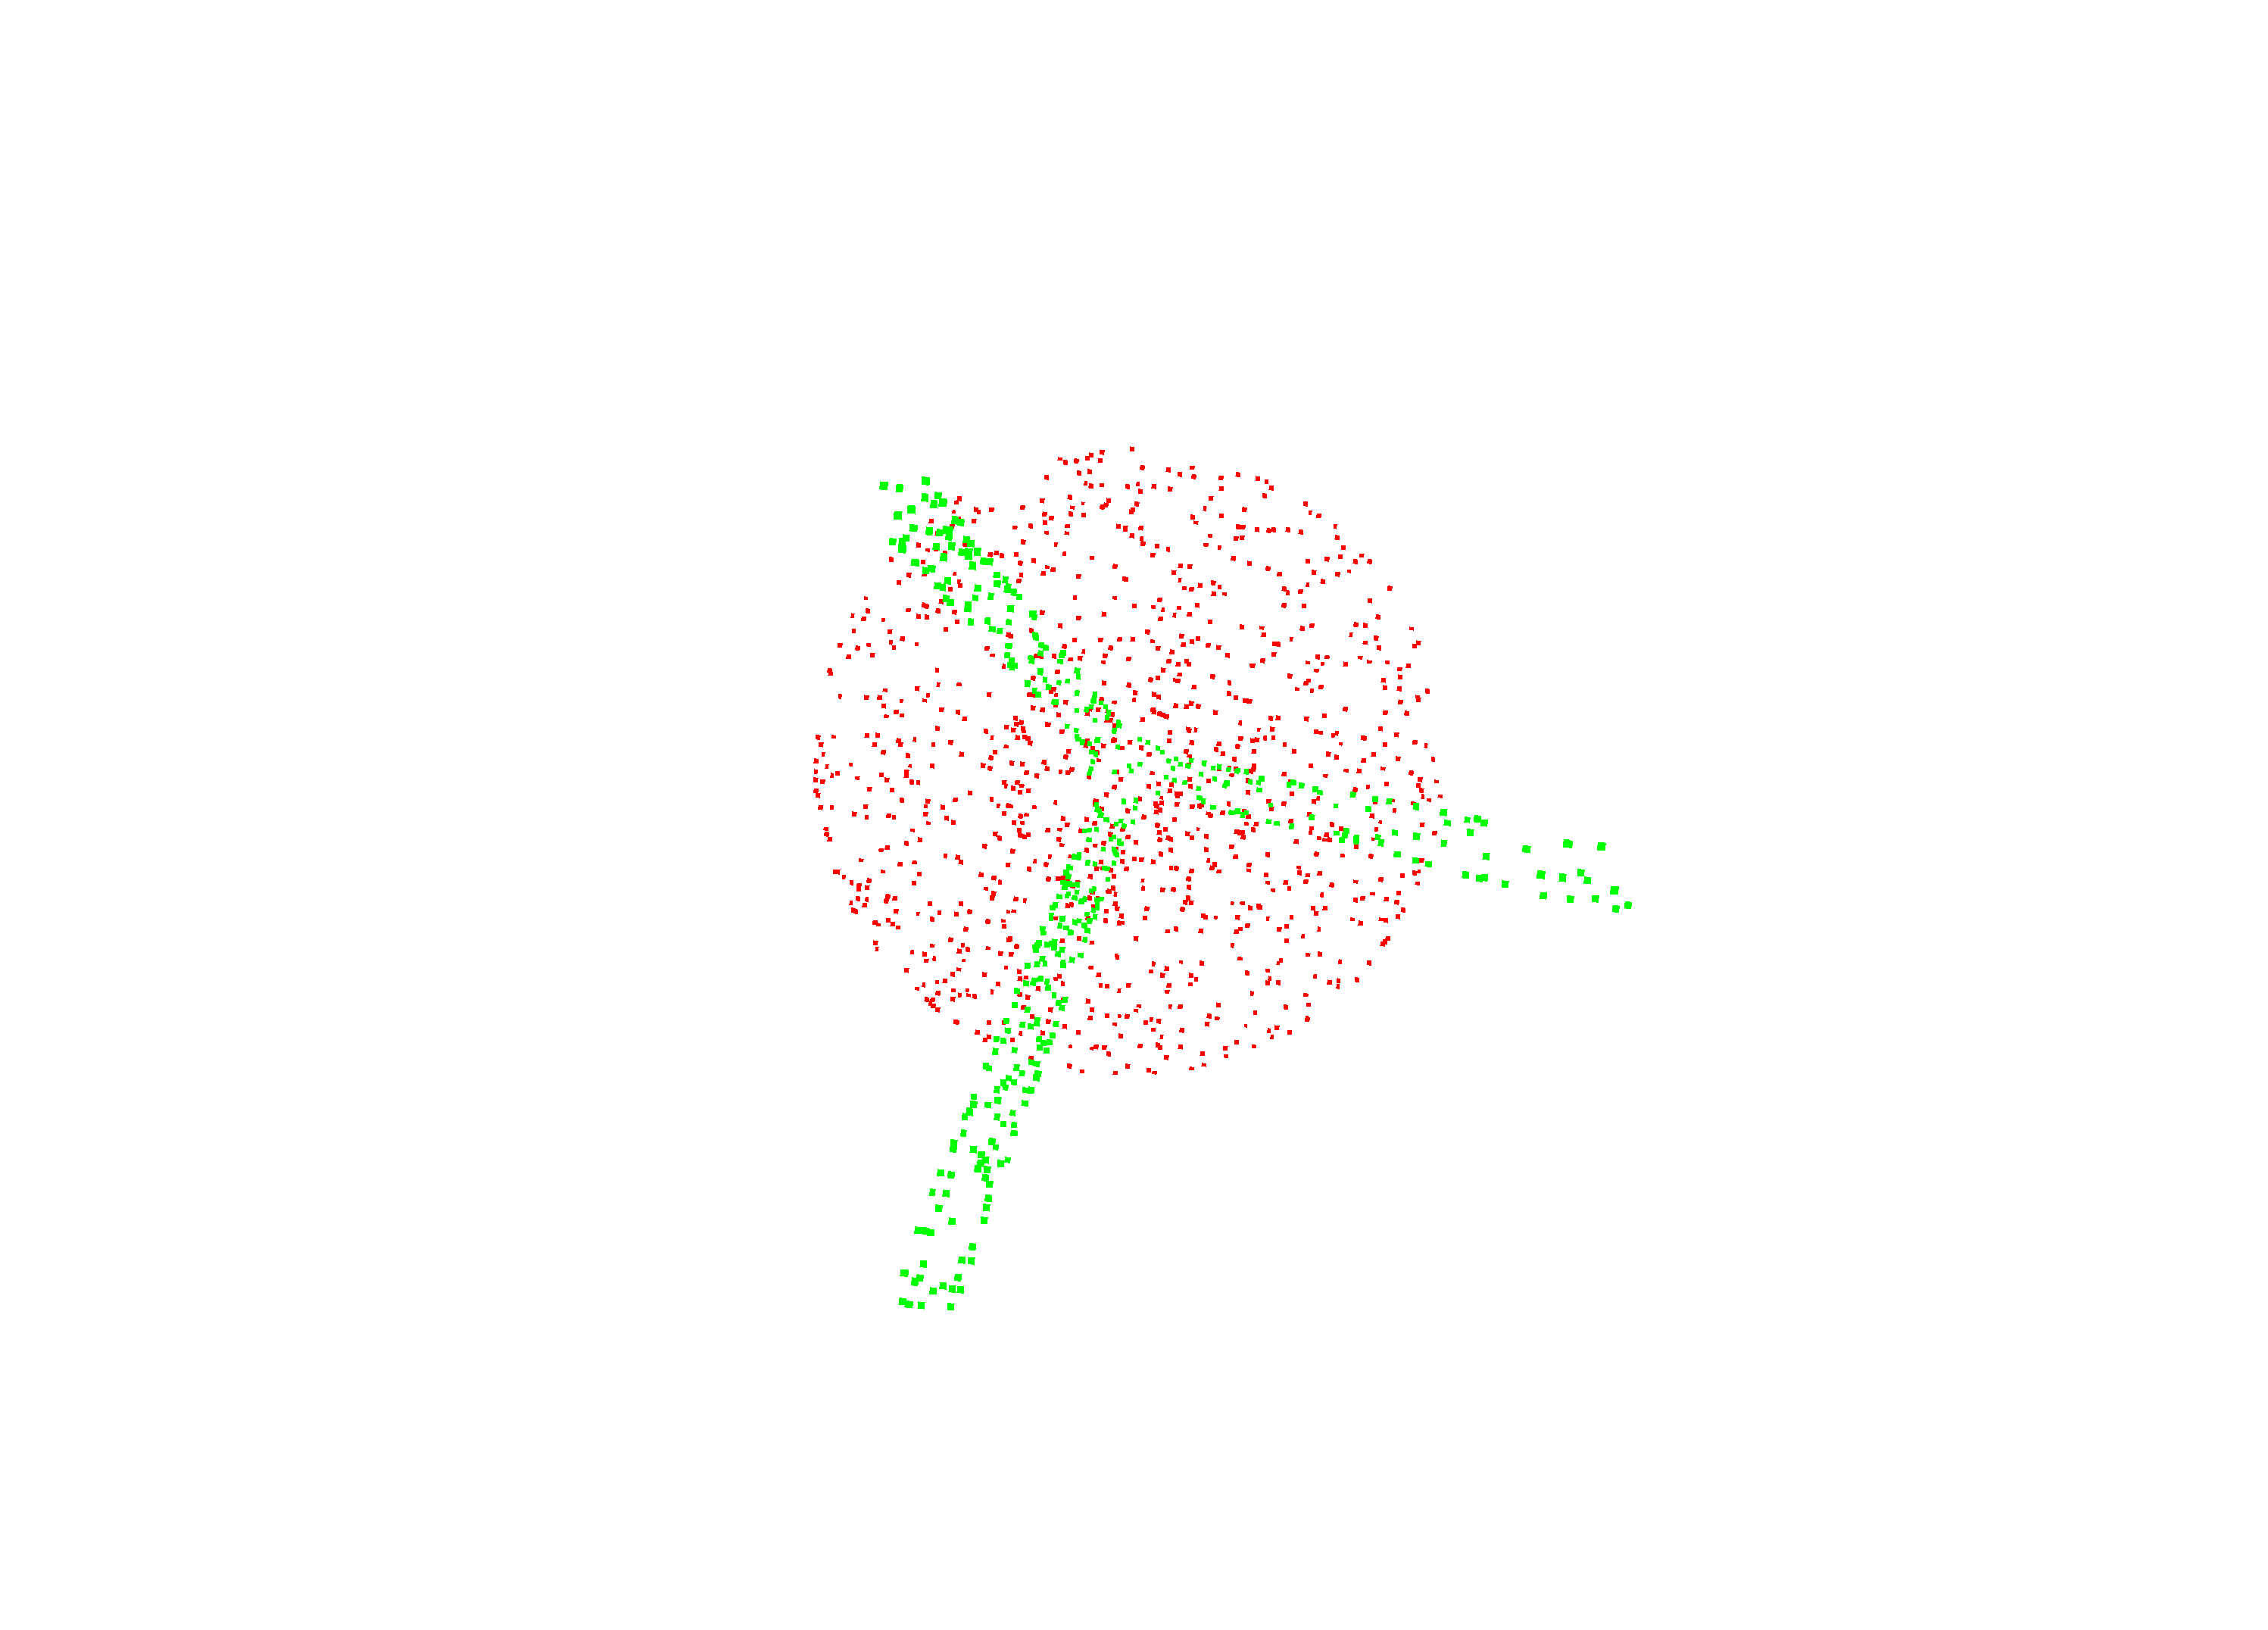
\includegraphics[width=\textwidth]{fig/supplement/part_segmentation/table/table01.pdf}
    \end{minipage}
    \hfill
    \begin{minipage}{0.25\textwidth}
        \centering
        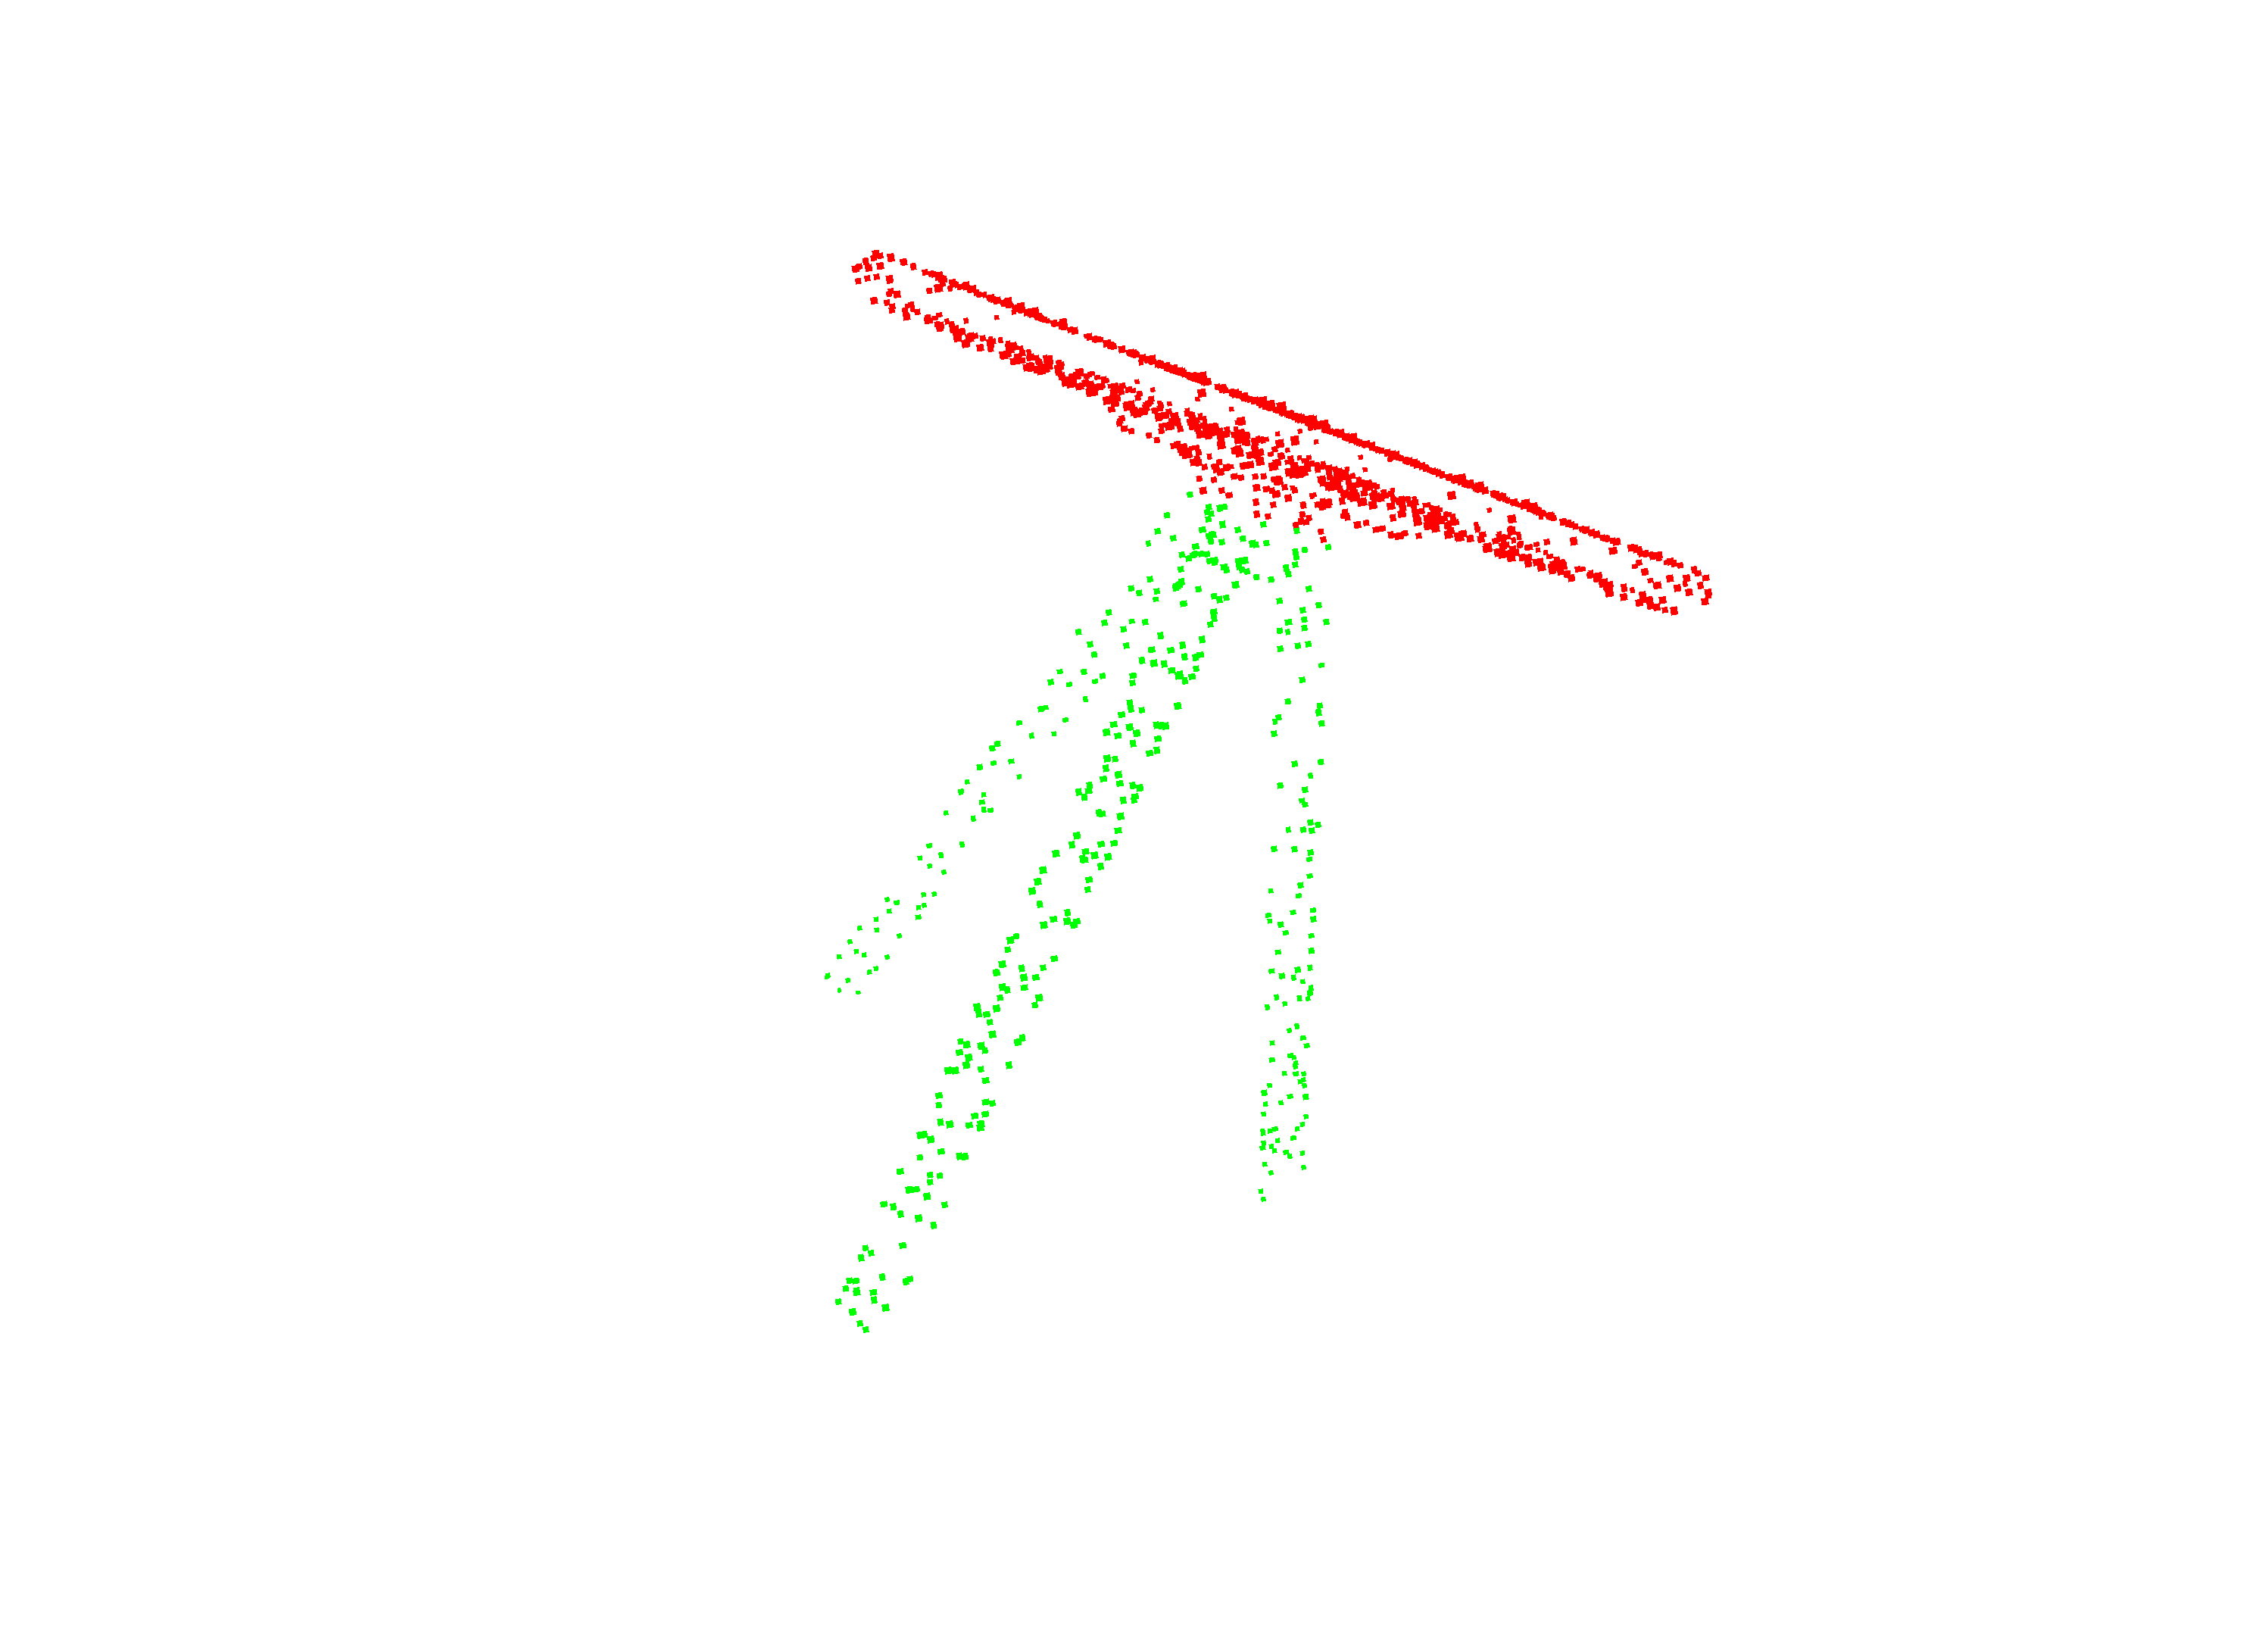
\includegraphics[width=\textwidth]{fig/supplement/part_segmentation/table/table02.pdf}
    \end{minipage}
    \hfill
    \caption{Qualitative results for part segmentation. We show our prediction projection images from three different viewpoints.}
    \label{fig:part_segmentation}
\end{figure*}



\begin{figure*}[htbp]
    \centering

    % 第一行左侧的竖排标签
    \begin{minipage}{0.09\textwidth}
        \centering
        Full
        Fine-tuning
    \end{minipage}
    \hfill
    % 第一行图片
    \begin{minipage}{0.22\textwidth}
        \centering
        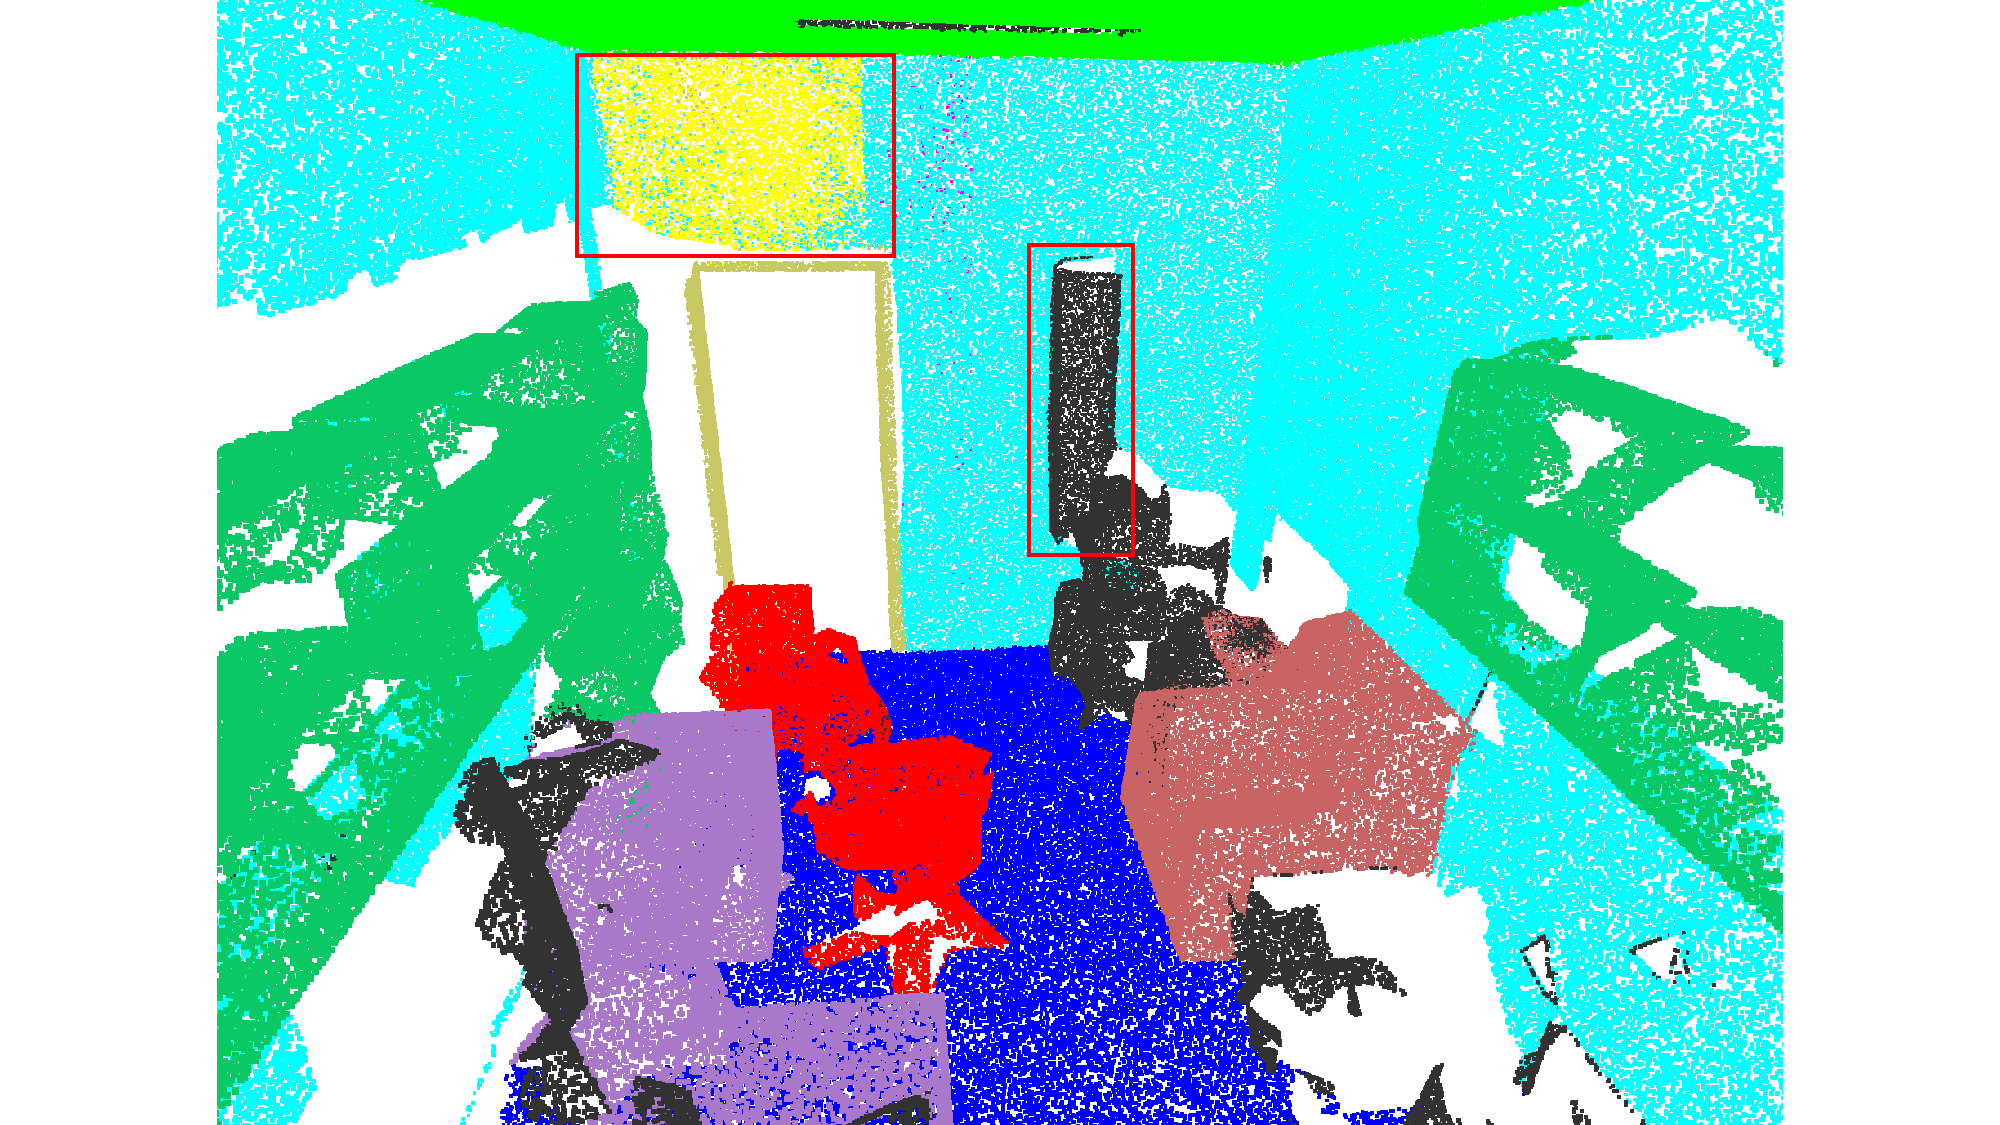
\includegraphics[width=\textwidth]{fig/supplement/semantic_segmentation/office_9/PT_office_9.pdf}
    \end{minipage}
    \hfill
    \begin{minipage}{0.22\textwidth}
        \centering
        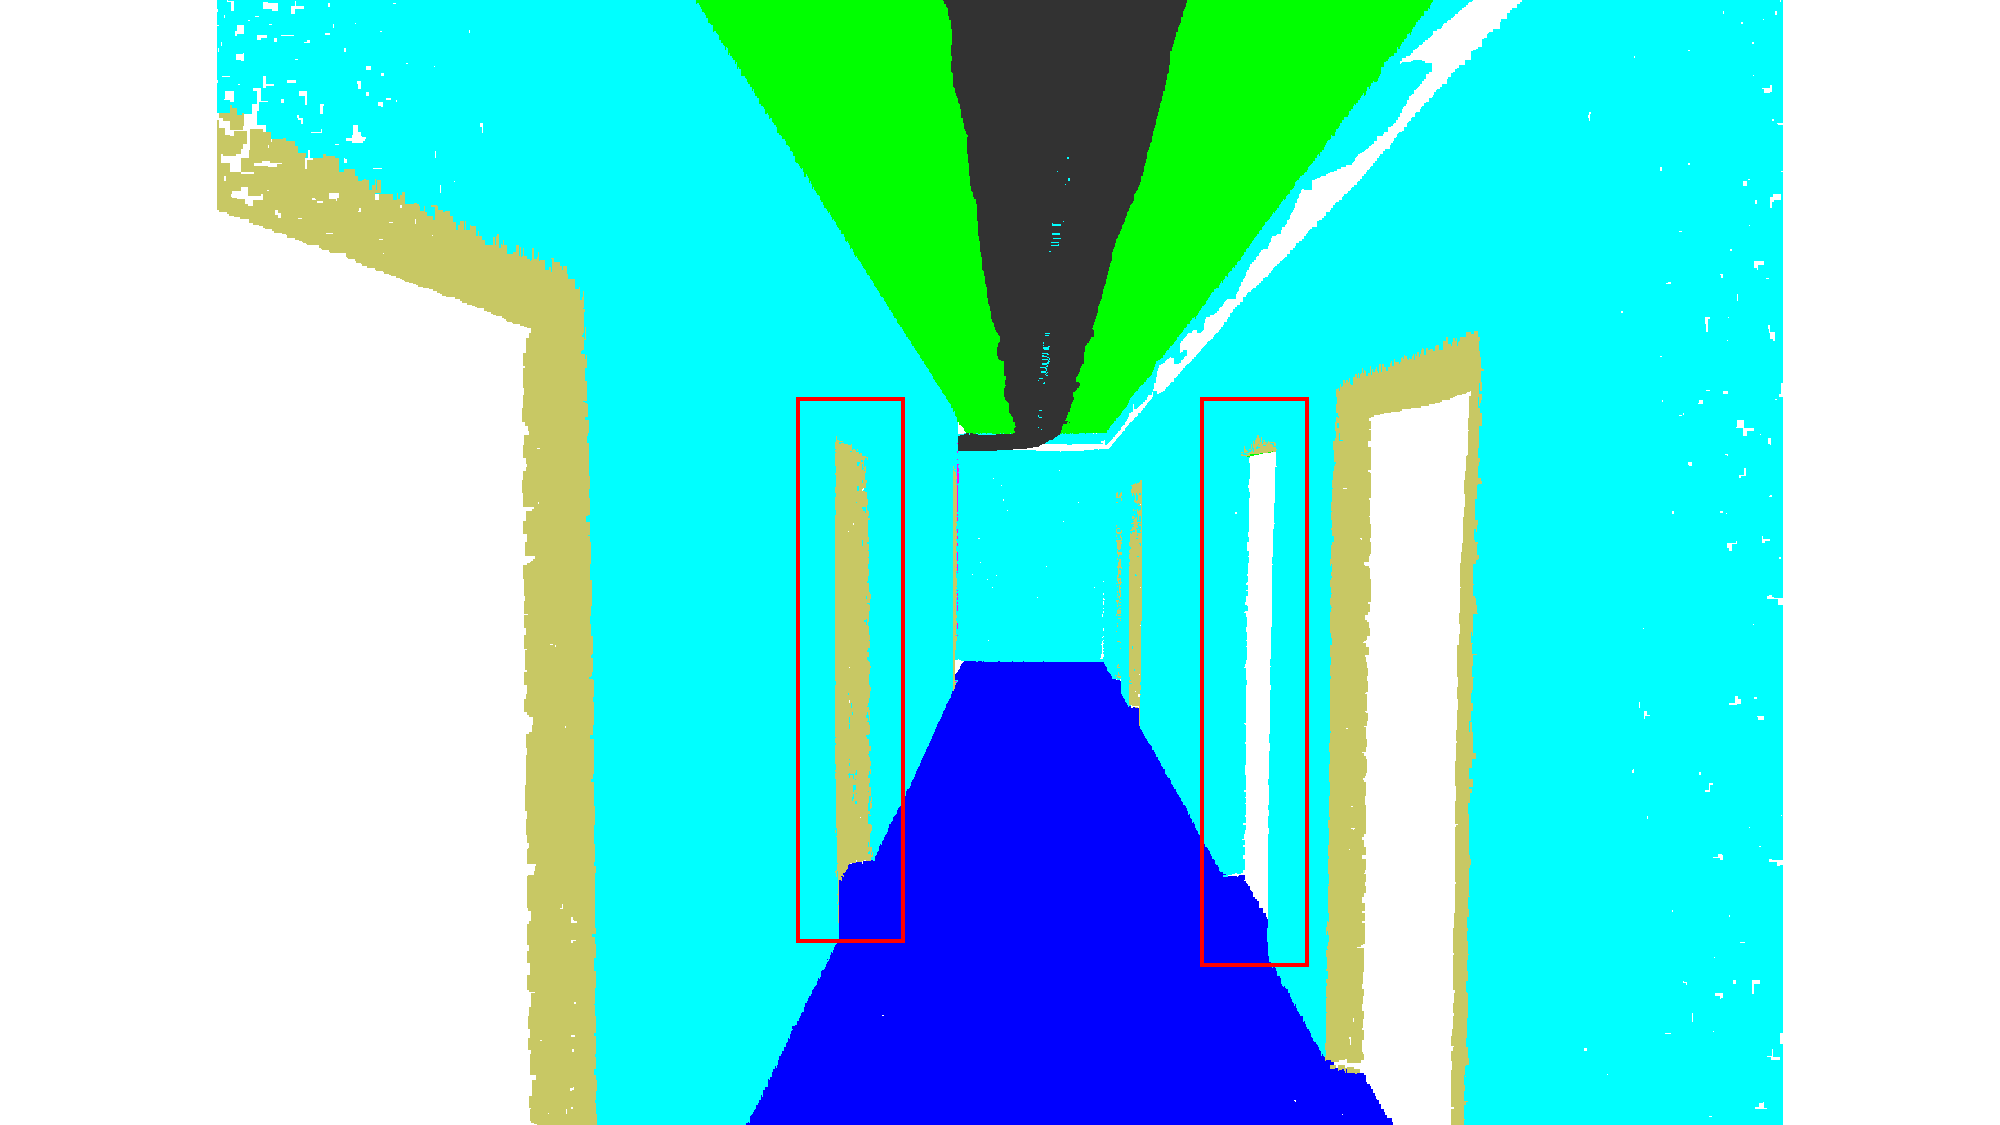
\includegraphics[width=\textwidth]{fig/supplement/semantic_segmentation/hallway_10/PT_hallway_10.pdf} % 替换为你的图片路径
    \end{minipage}
    \hfill
    \begin{minipage}{0.22\textwidth}
        \centering
        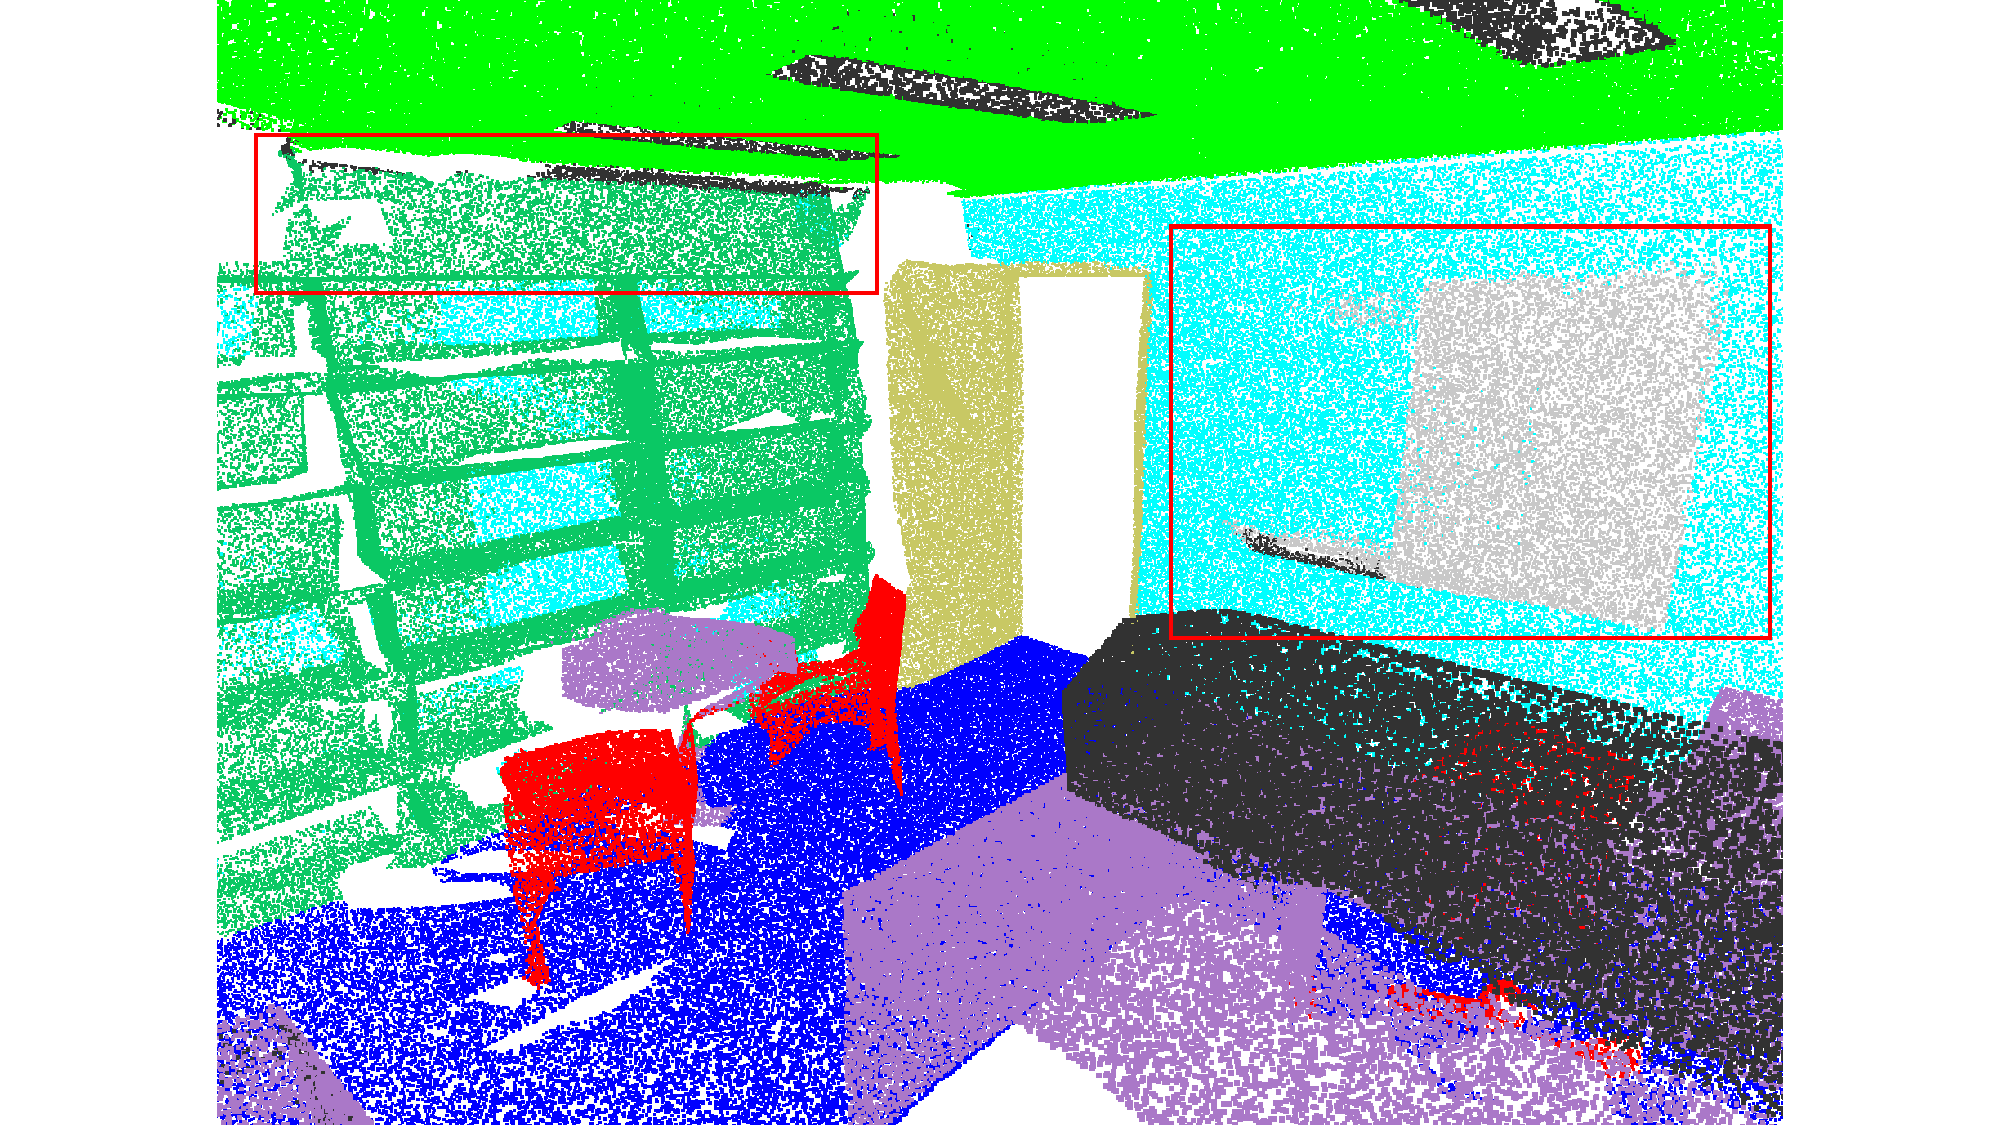
\includegraphics[width=\textwidth]{fig/supplement/semantic_segmentation/office_35/PT_office_35.pdf}
    \end{minipage}
    \hfill
    \begin{minipage}{0.22\textwidth}
        \centering
        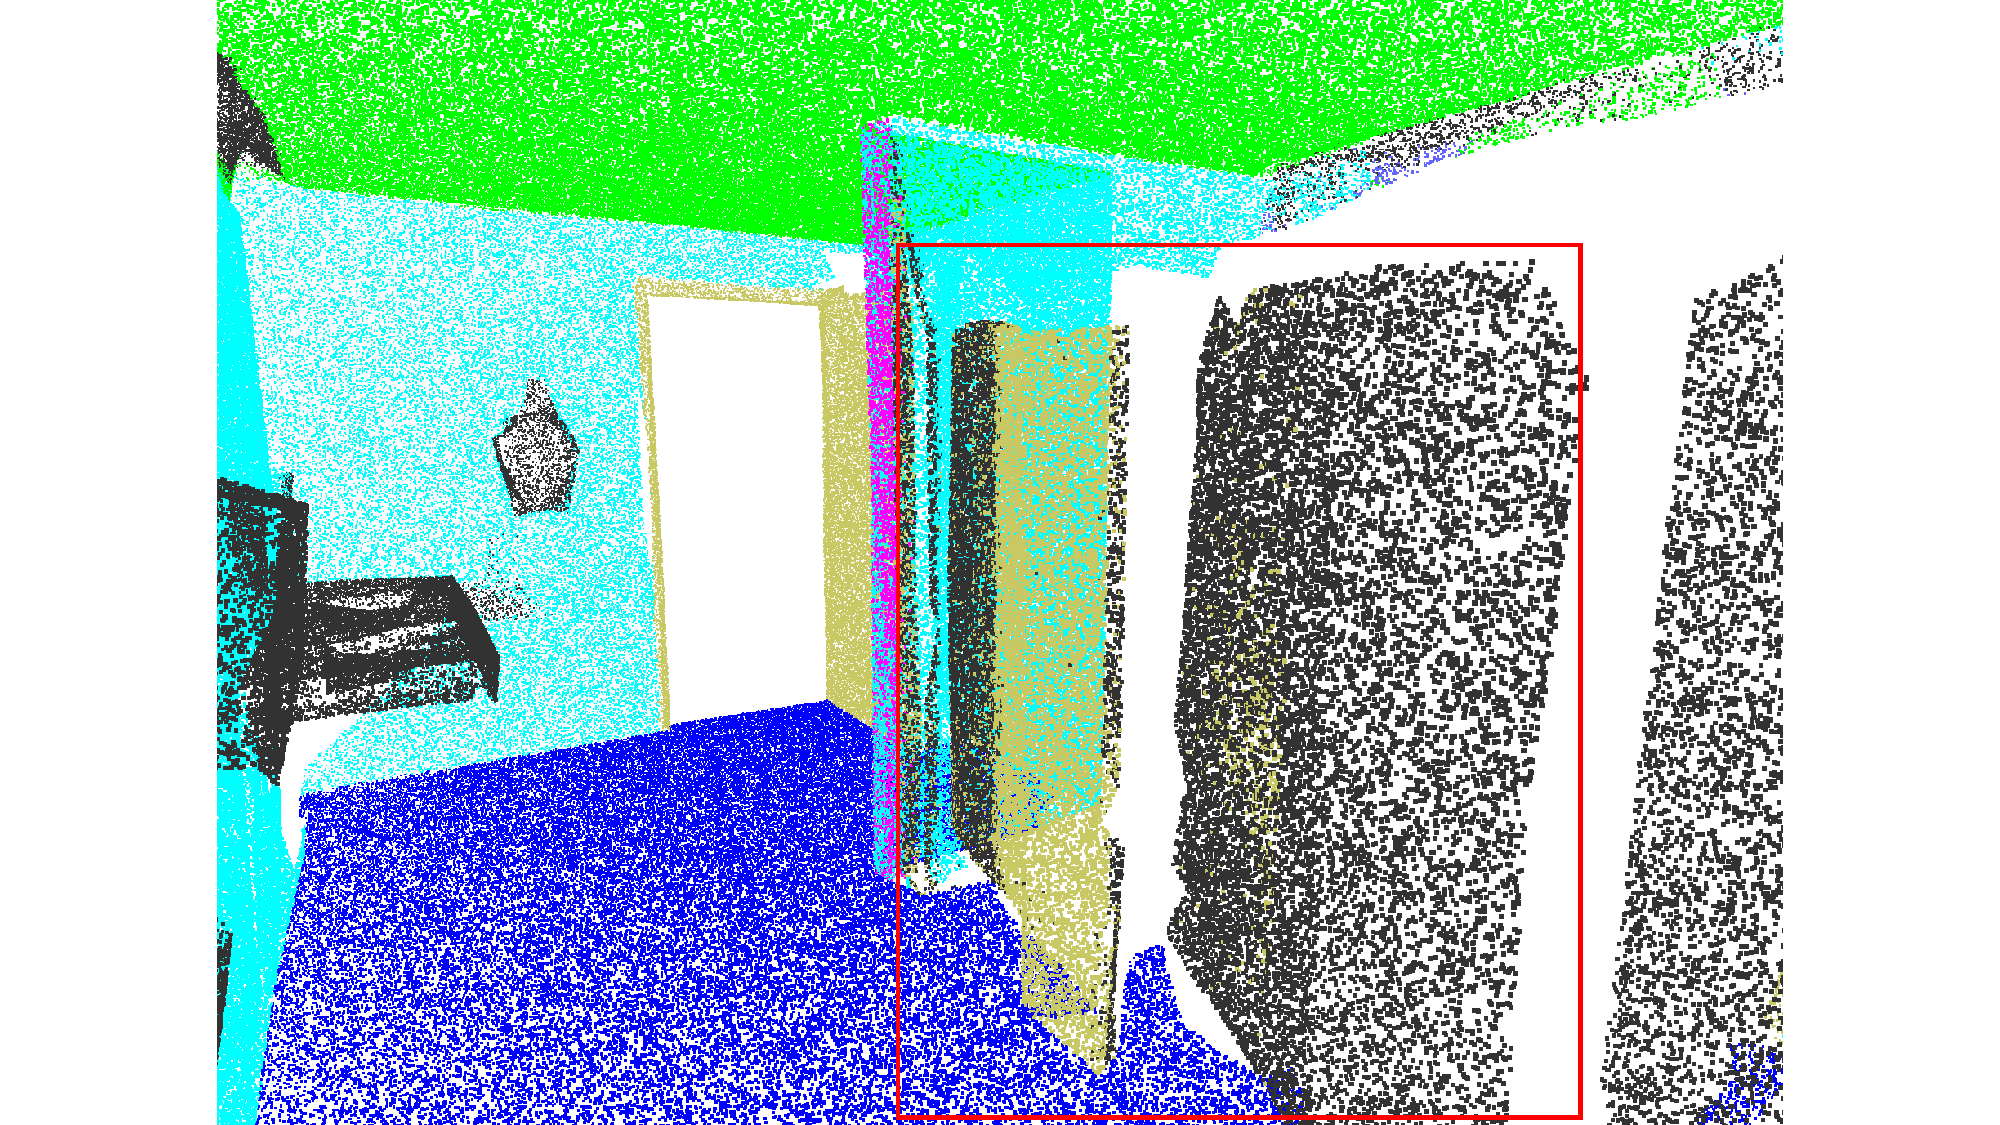
\includegraphics[width=\textwidth]{fig/supplement/semantic_segmentation/wc_2/PT_wc_2.pdf}
    \end{minipage}
    \hfill

    % 换行
    \vspace{0.5em}

    % 第二行左侧的竖排标签
    \begin{minipage}{0.09\textwidth}
        \centering
        DAPT
    \end{minipage}
    \hfill
    % 第二行图片
    \begin{minipage}{0.22\textwidth}
        \centering
        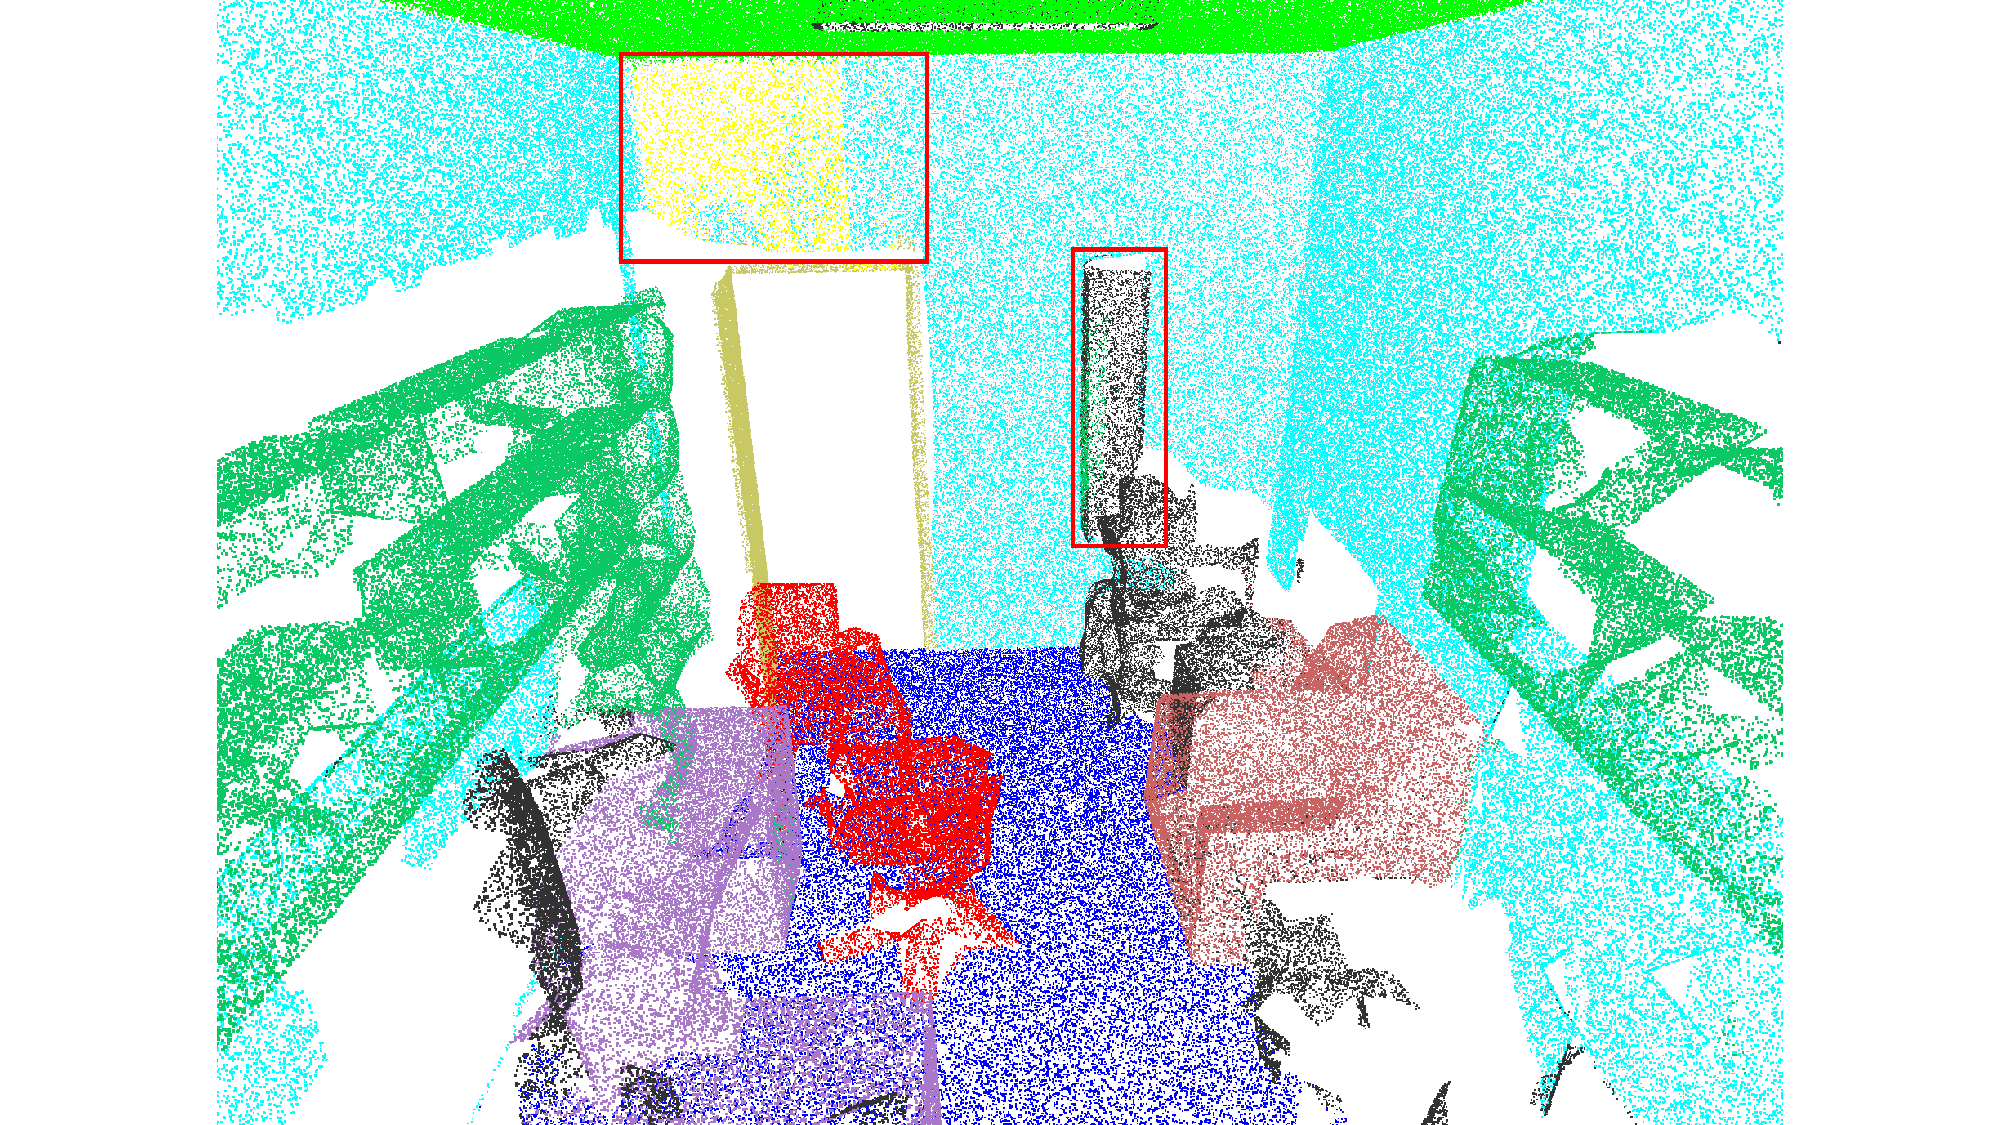
\includegraphics[width=\textwidth]{fig/supplement/semantic_segmentation/office_9/DAPT_office_9.pdf}
    \end{minipage}
    \hfill
    \begin{minipage}{0.22\textwidth}
        \centering
        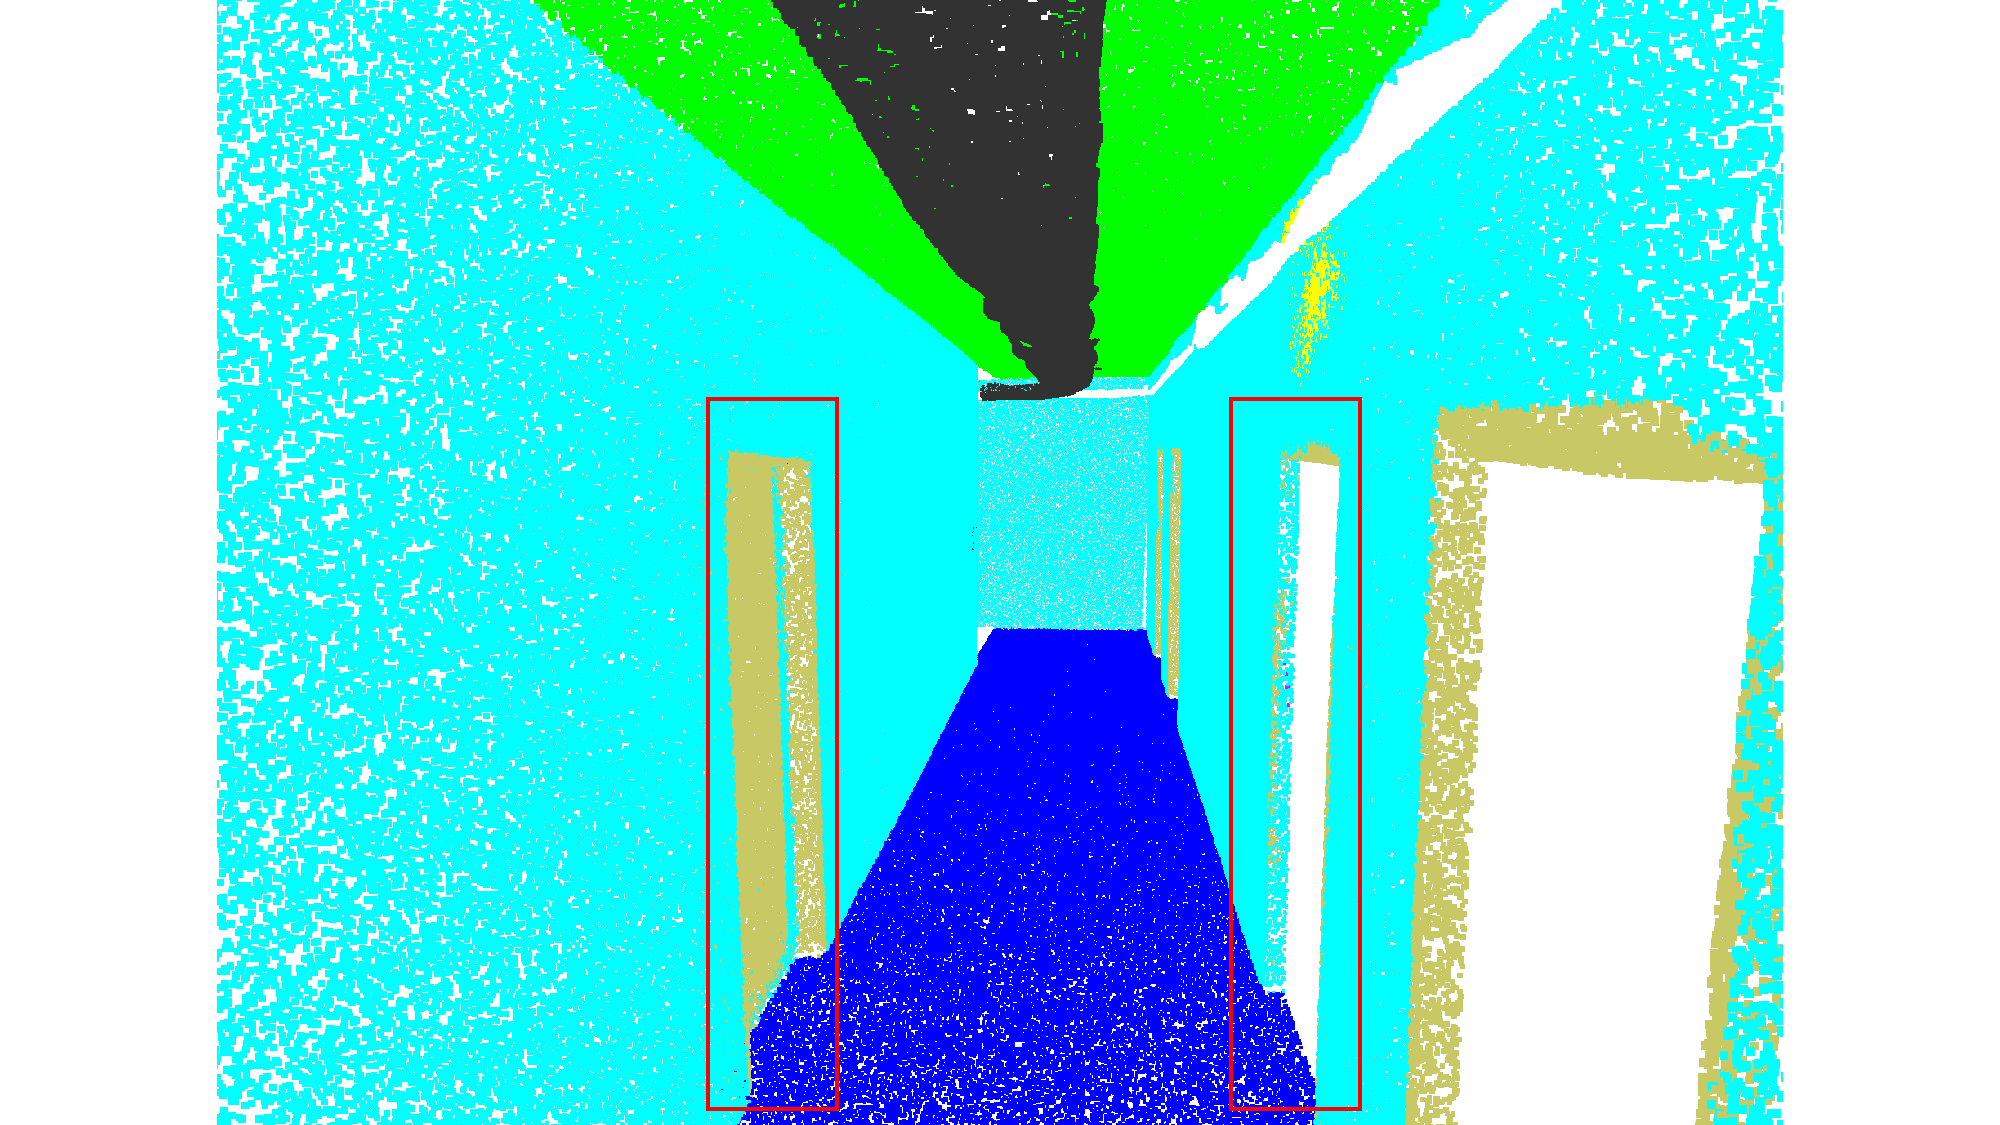
\includegraphics[width=\textwidth]{fig/supplement/semantic_segmentation/hallway_10/DAPT_hallway_10.pdf}
    \end{minipage}
    \hfill
    \begin{minipage}{0.22\textwidth}
        \centering
        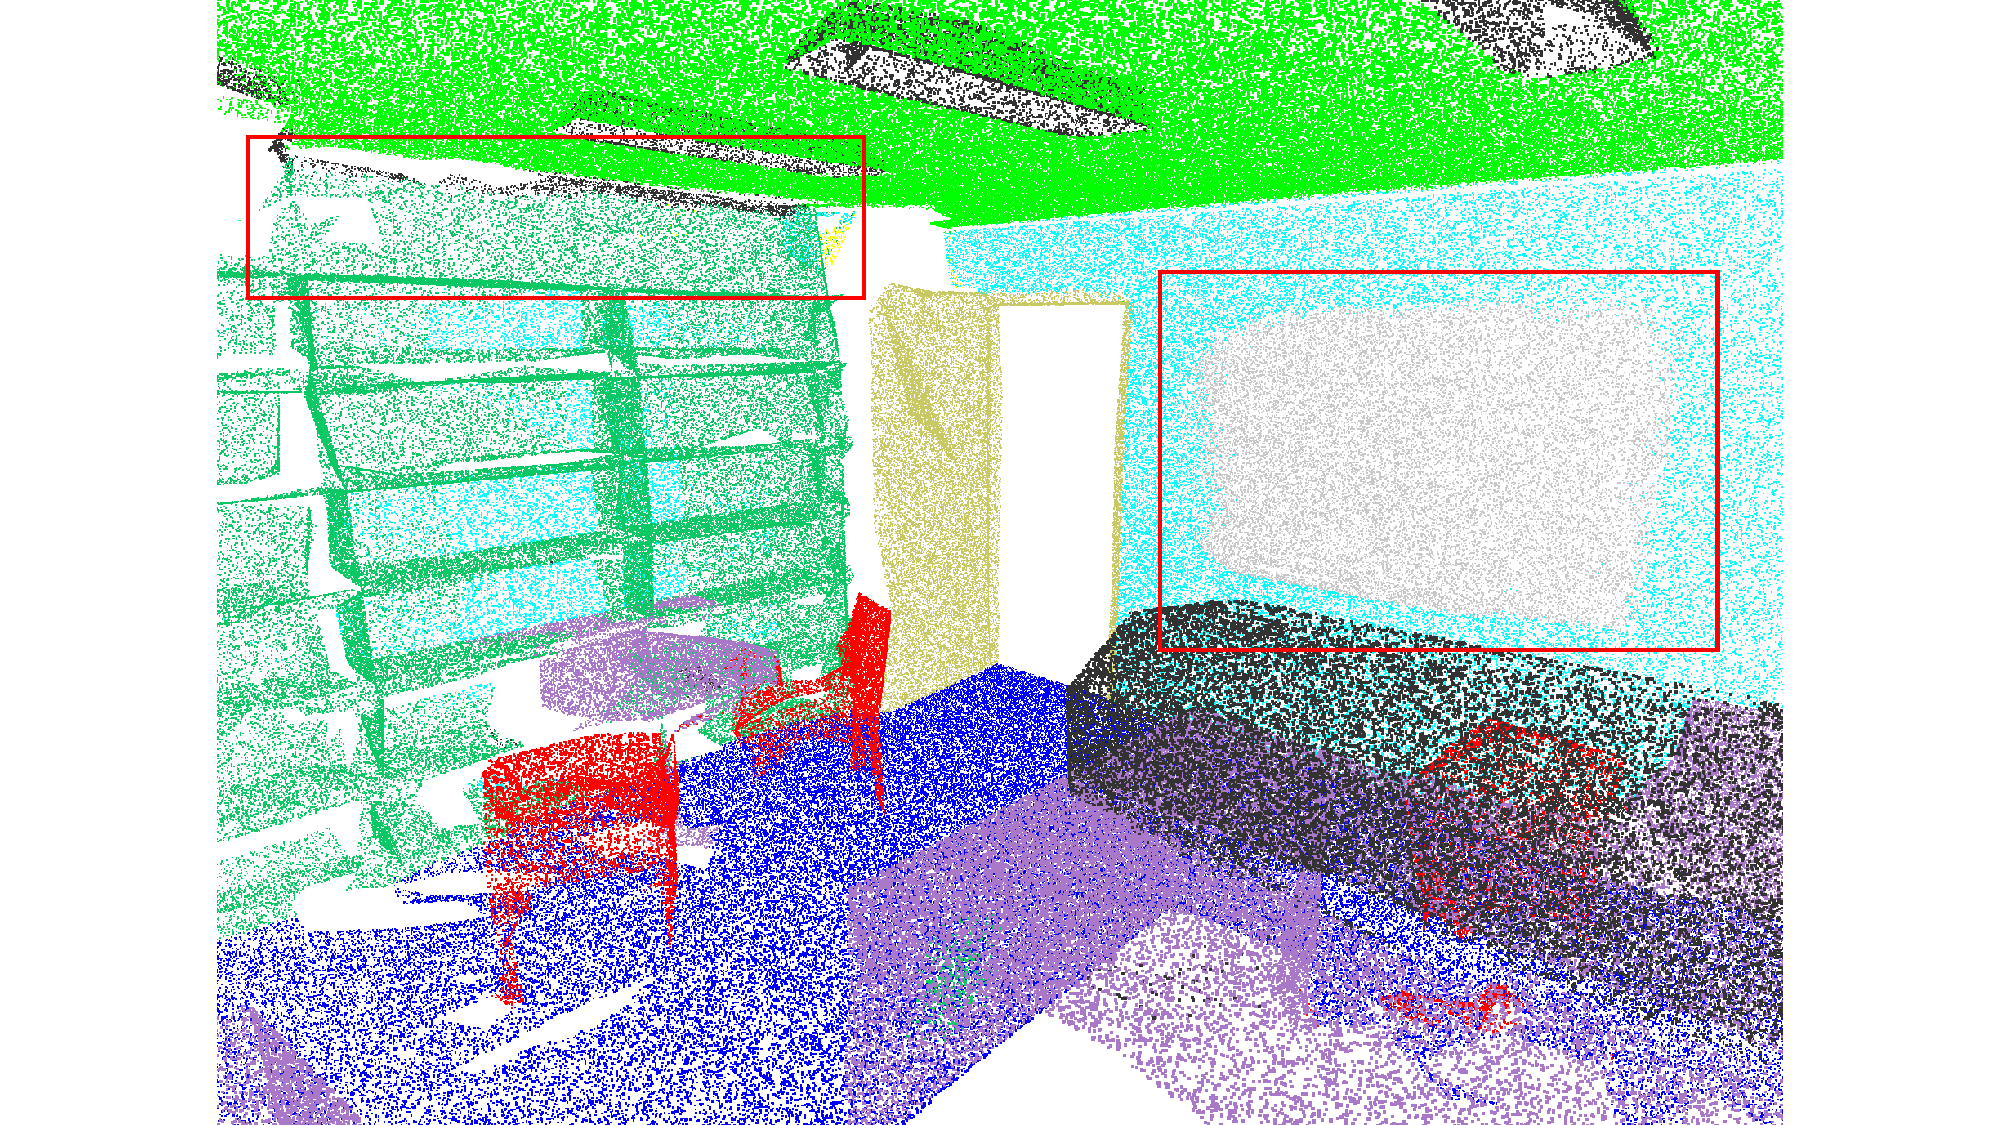
\includegraphics[width=\textwidth]{fig/supplement/semantic_segmentation/office_35/DAPT_office_35.pdf}
    \end{minipage}
    \hfill
    \begin{minipage}{0.22\textwidth}
        \centering
        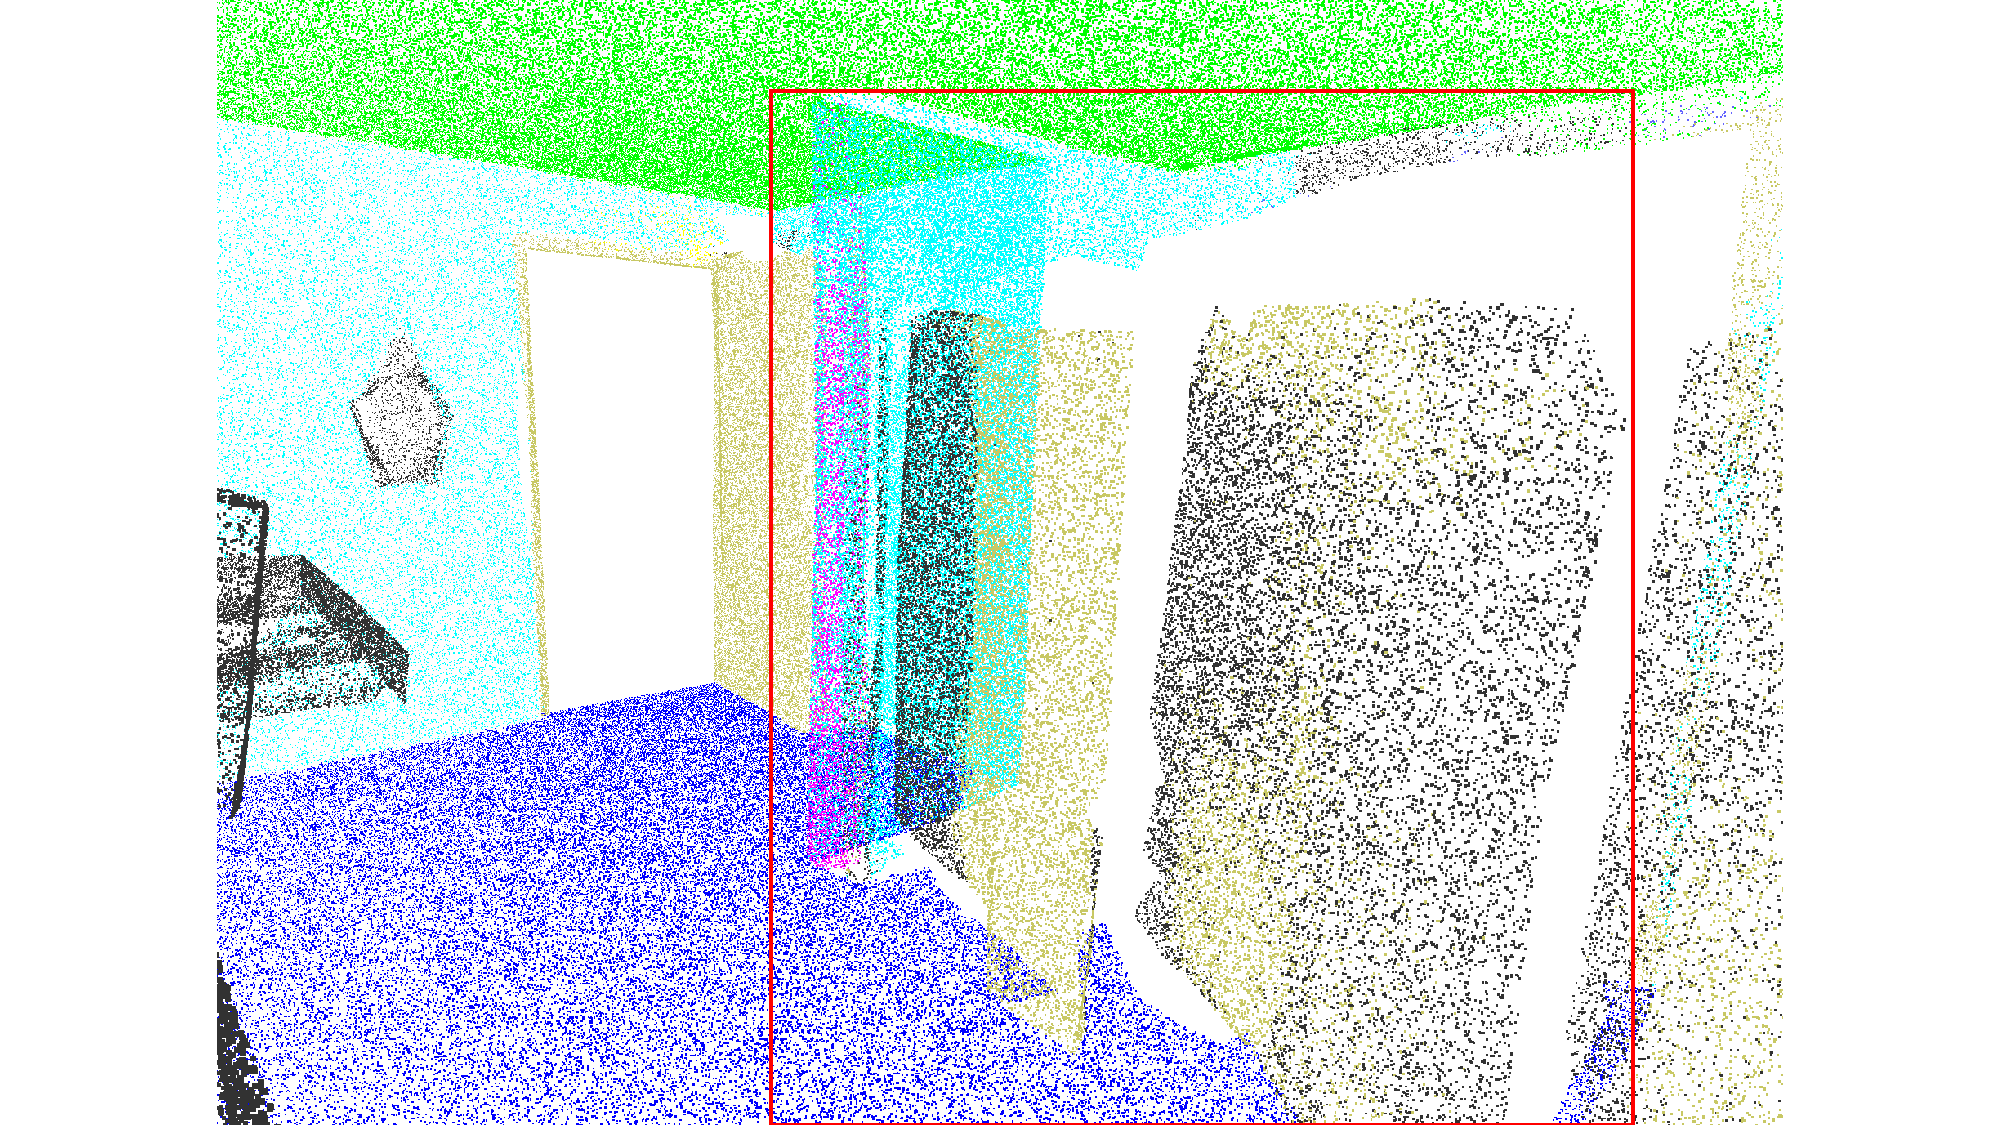
\includegraphics[width=\textwidth]{fig/supplement/semantic_segmentation/wc_2/DAPT_wc_2.pdf}
    \end{minipage}
    \hfill

    % 换行
    \vspace{0.5em}

    % 第三行左侧的竖排标签
    \begin{minipage}{0.09\textwidth}
        \centering
        IDPT
    \end{minipage}
    \hfill
    % 第三行图片
    \begin{minipage}{0.22\textwidth}
        \centering
        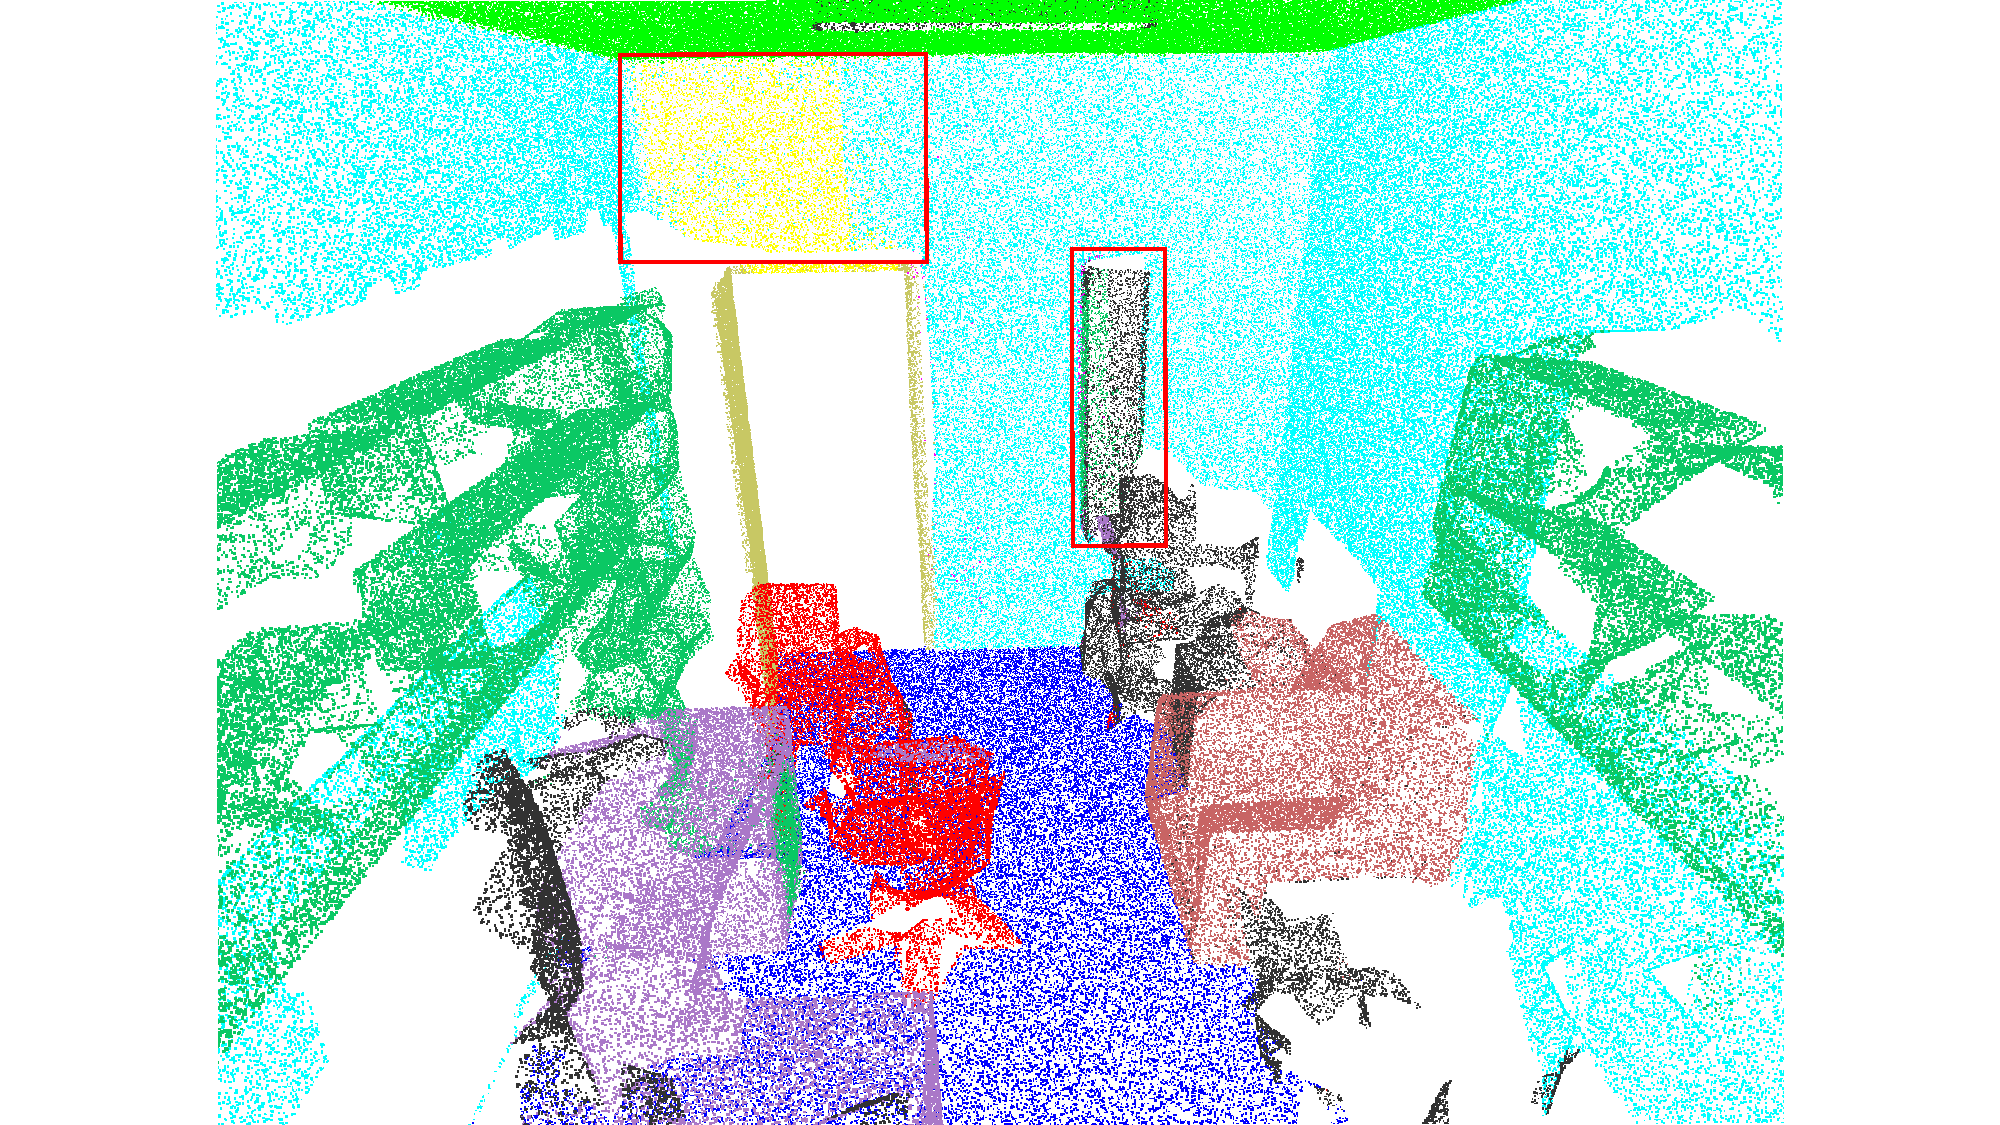
\includegraphics[width=\textwidth]{fig/supplement/semantic_segmentation/office_9/IDPT_office_9.pdf}
    \end{minipage}
    \hfill
    \begin{minipage}{0.22\textwidth}
        \centering
        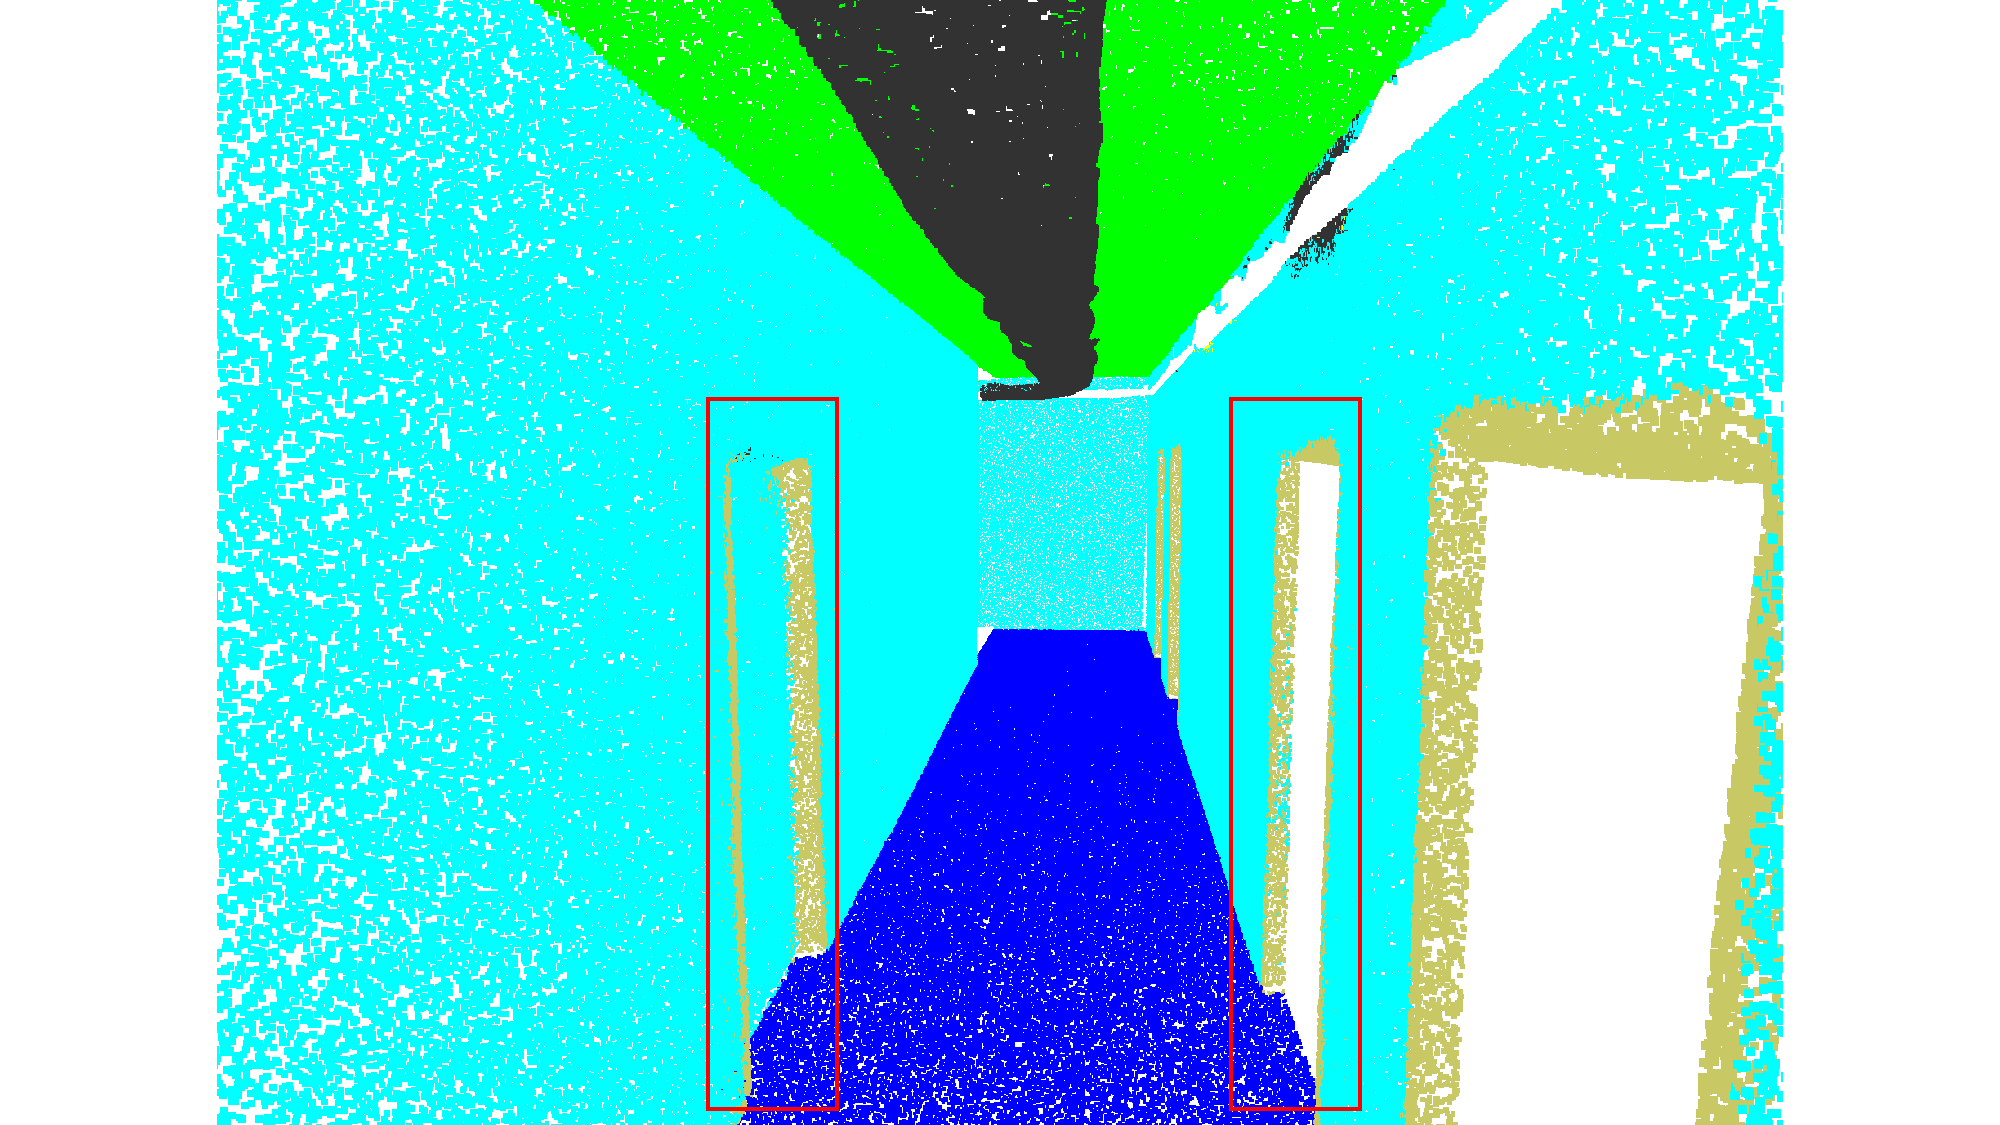
\includegraphics[width=\textwidth]{fig/supplement/semantic_segmentation/hallway_10/IDPT_hallway_10.pdf}
    \end{minipage}
    \hfill
    \begin{minipage}{0.22\textwidth}
        \centering
        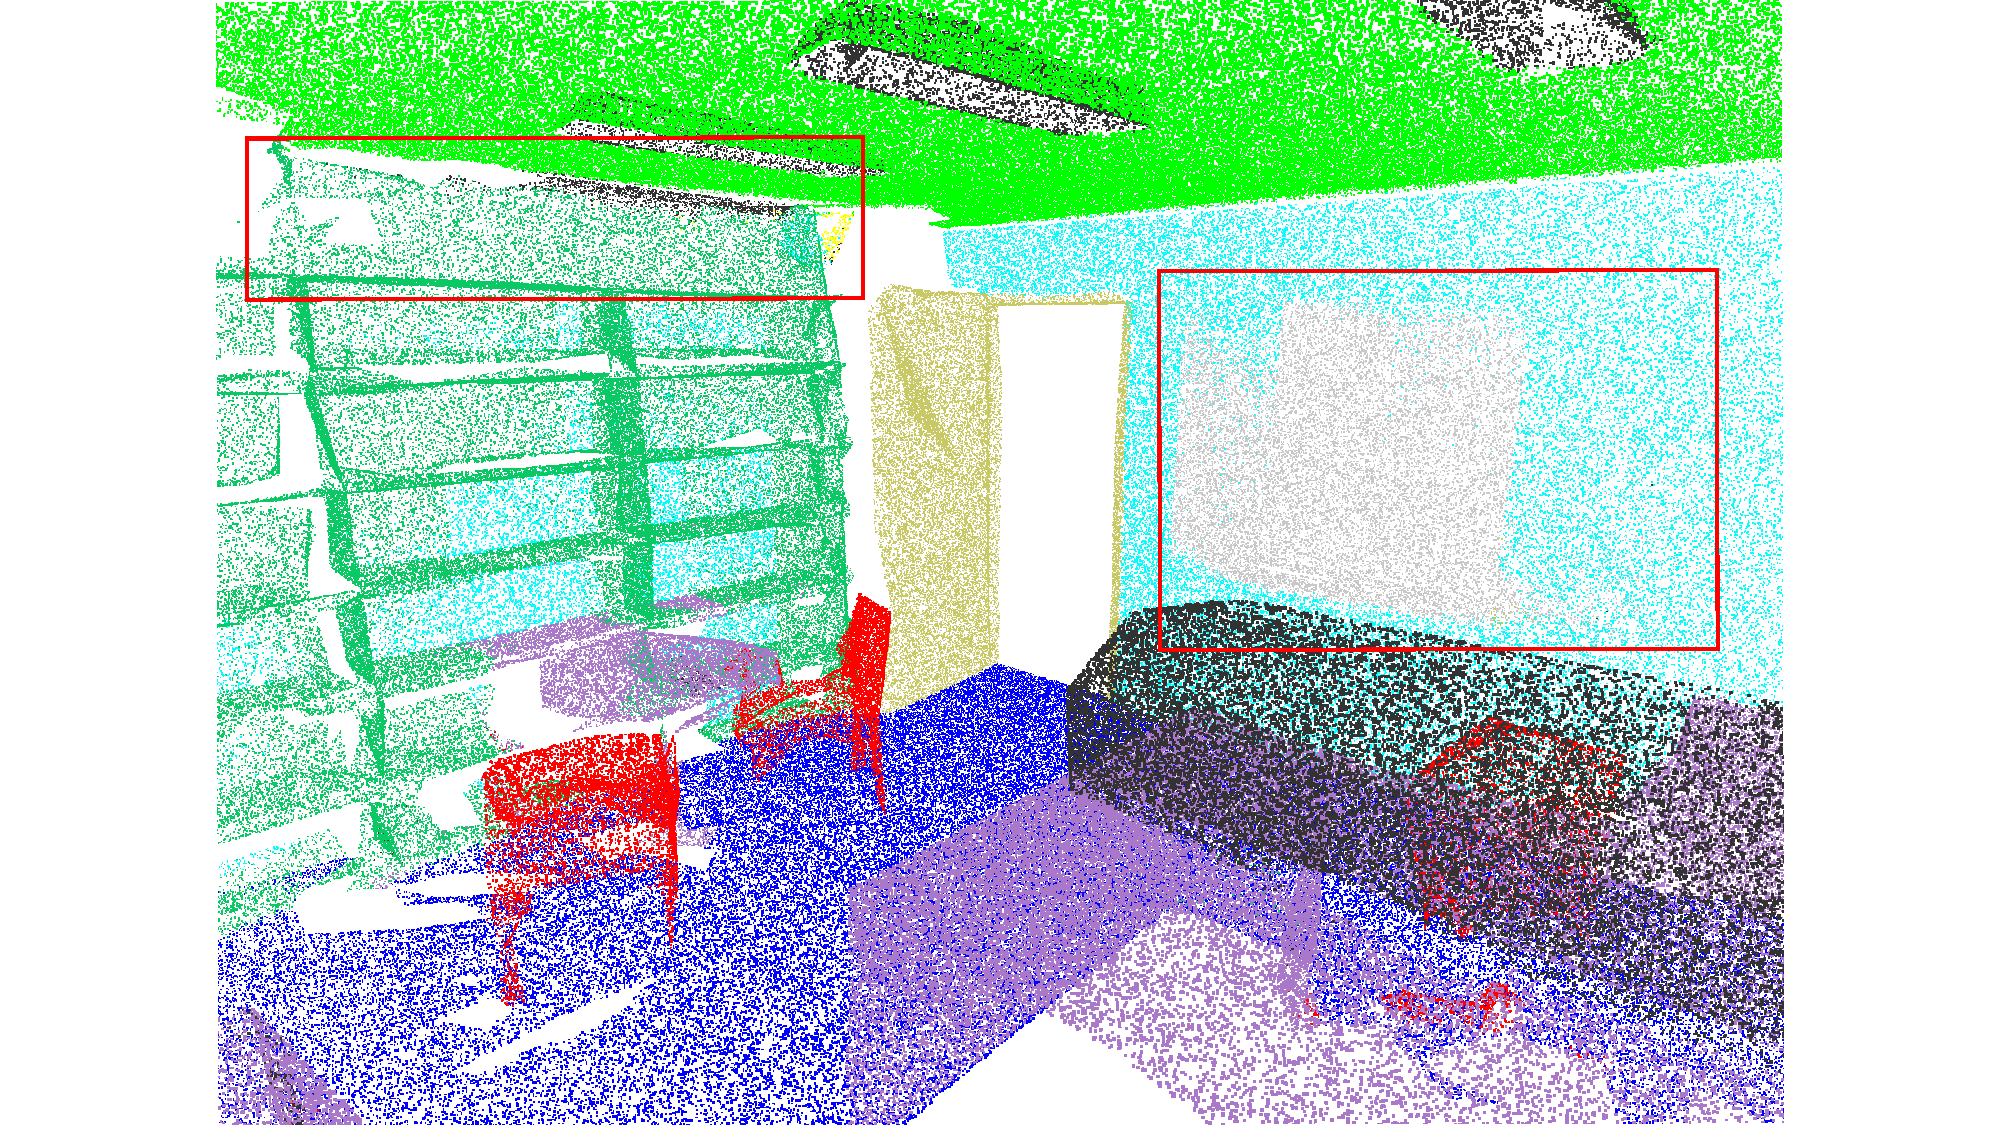
\includegraphics[width=\textwidth]{fig/supplement/semantic_segmentation/office_35/IDPT_office_35.pdf}
    \end{minipage}
    \hfill
    \begin{minipage}{0.22\textwidth}
        \centering
        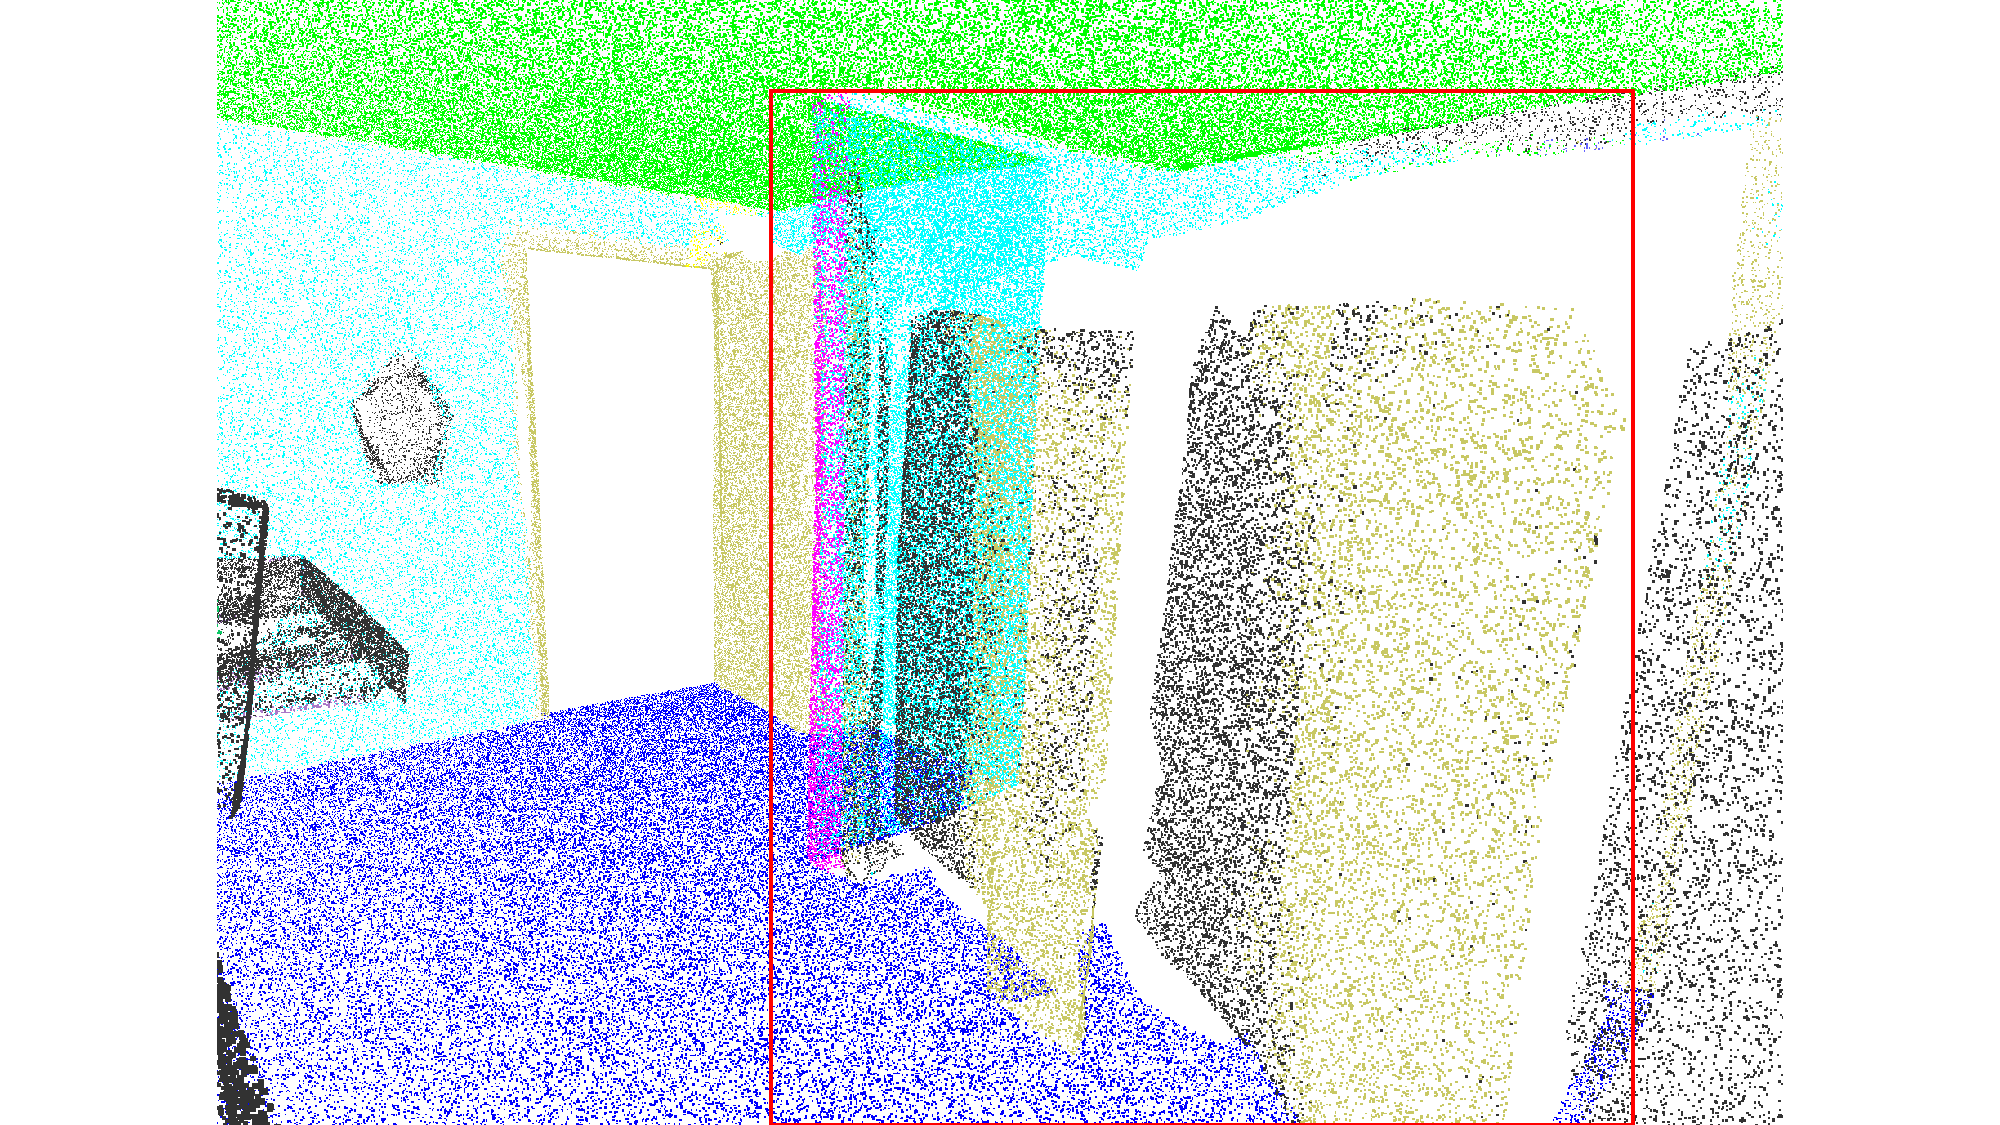
\includegraphics[width=\textwidth]{fig/supplement/semantic_segmentation/wc_2/IDPT_wc_2.pdf}
    \end{minipage}
    \hfill

    % 换行
    \vspace{0.5em}

    % 第四行左侧的竖排标签
    \begin{minipage}{0.09\textwidth}
        \centering
        PPT
    \end{minipage}
    \hfill
    % 第四行图片
    \begin{minipage}{0.22\textwidth}
        \centering
        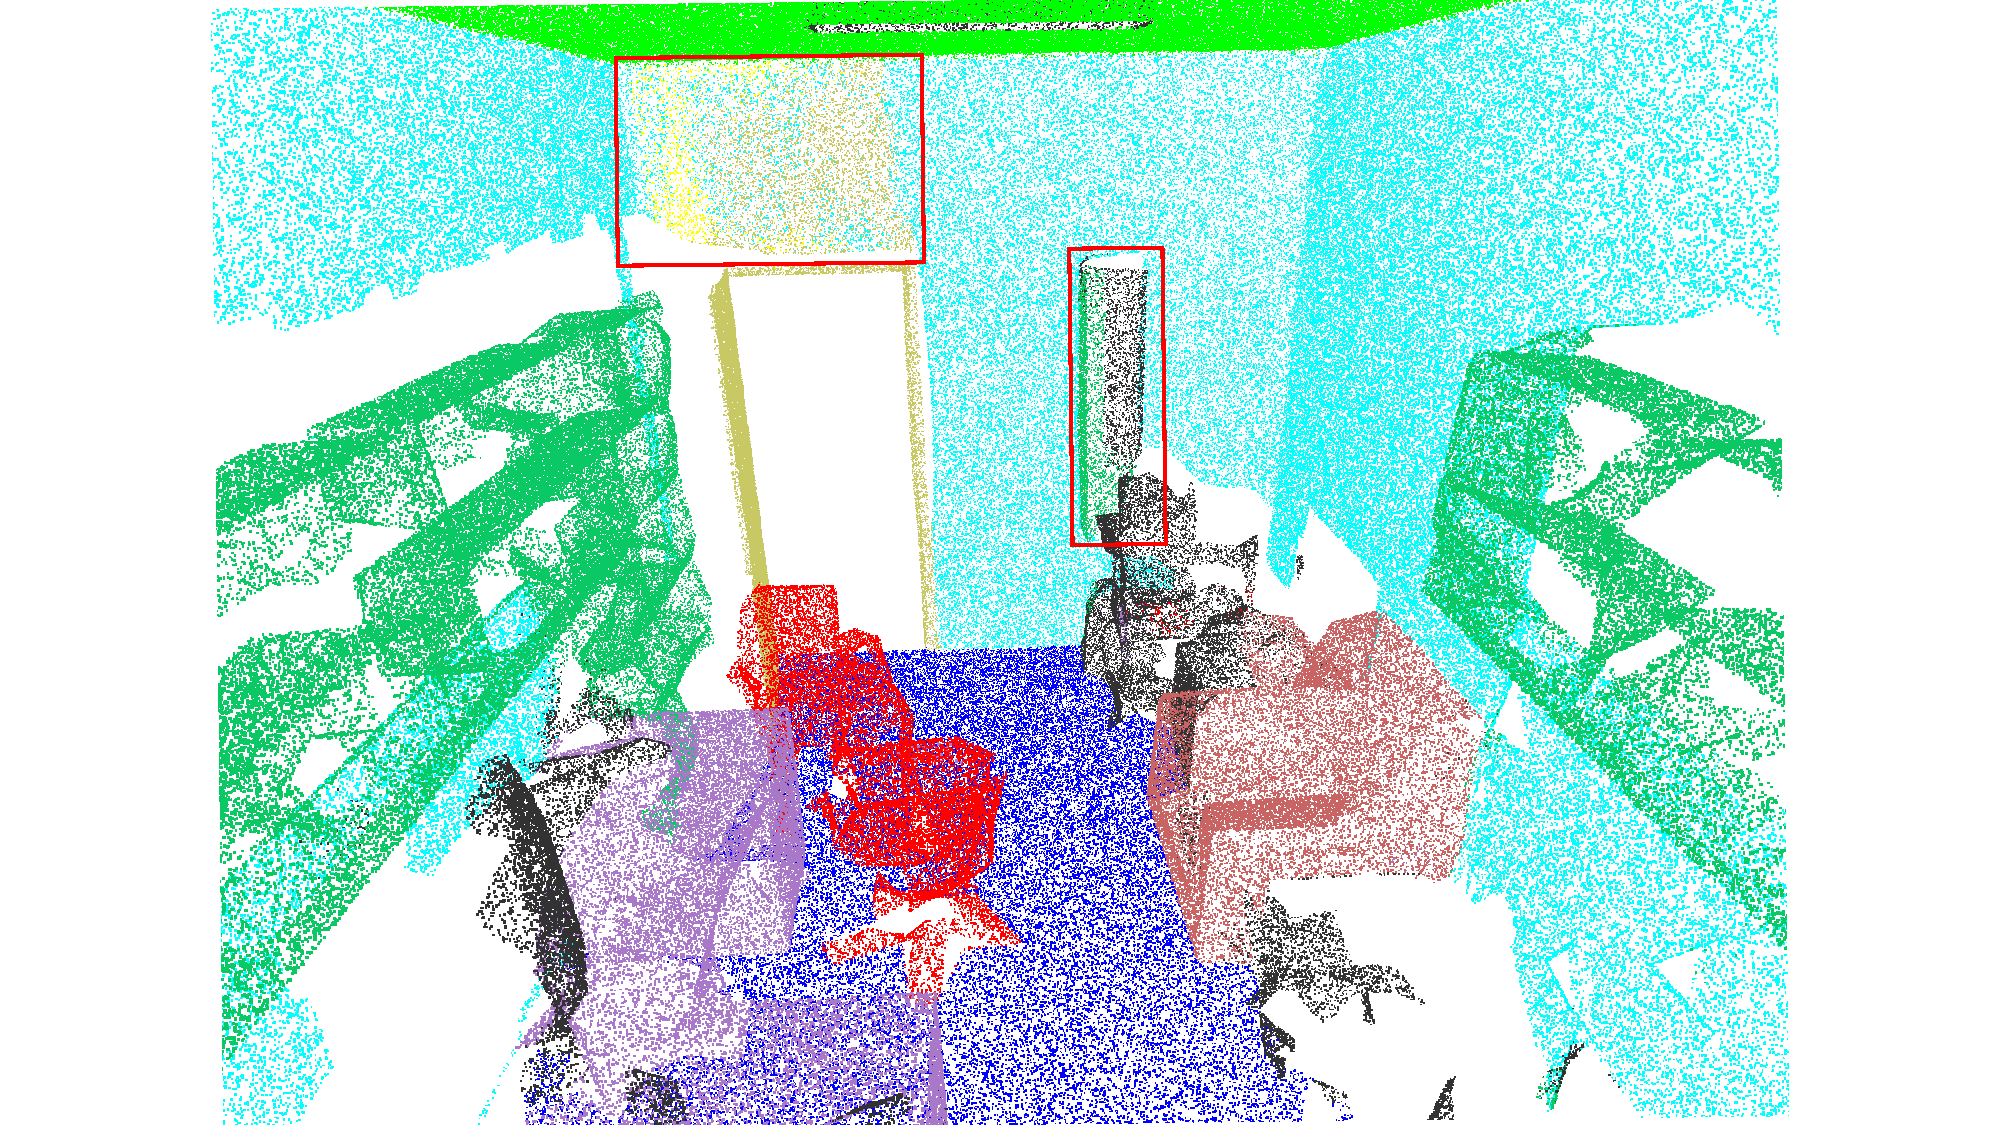
\includegraphics[width=\textwidth]{fig/supplement/semantic_segmentation/office_9/PPT_office_9.pdf}
    \end{minipage}
    \hfill
     \begin{minipage}{0.22\textwidth}
        \centering
        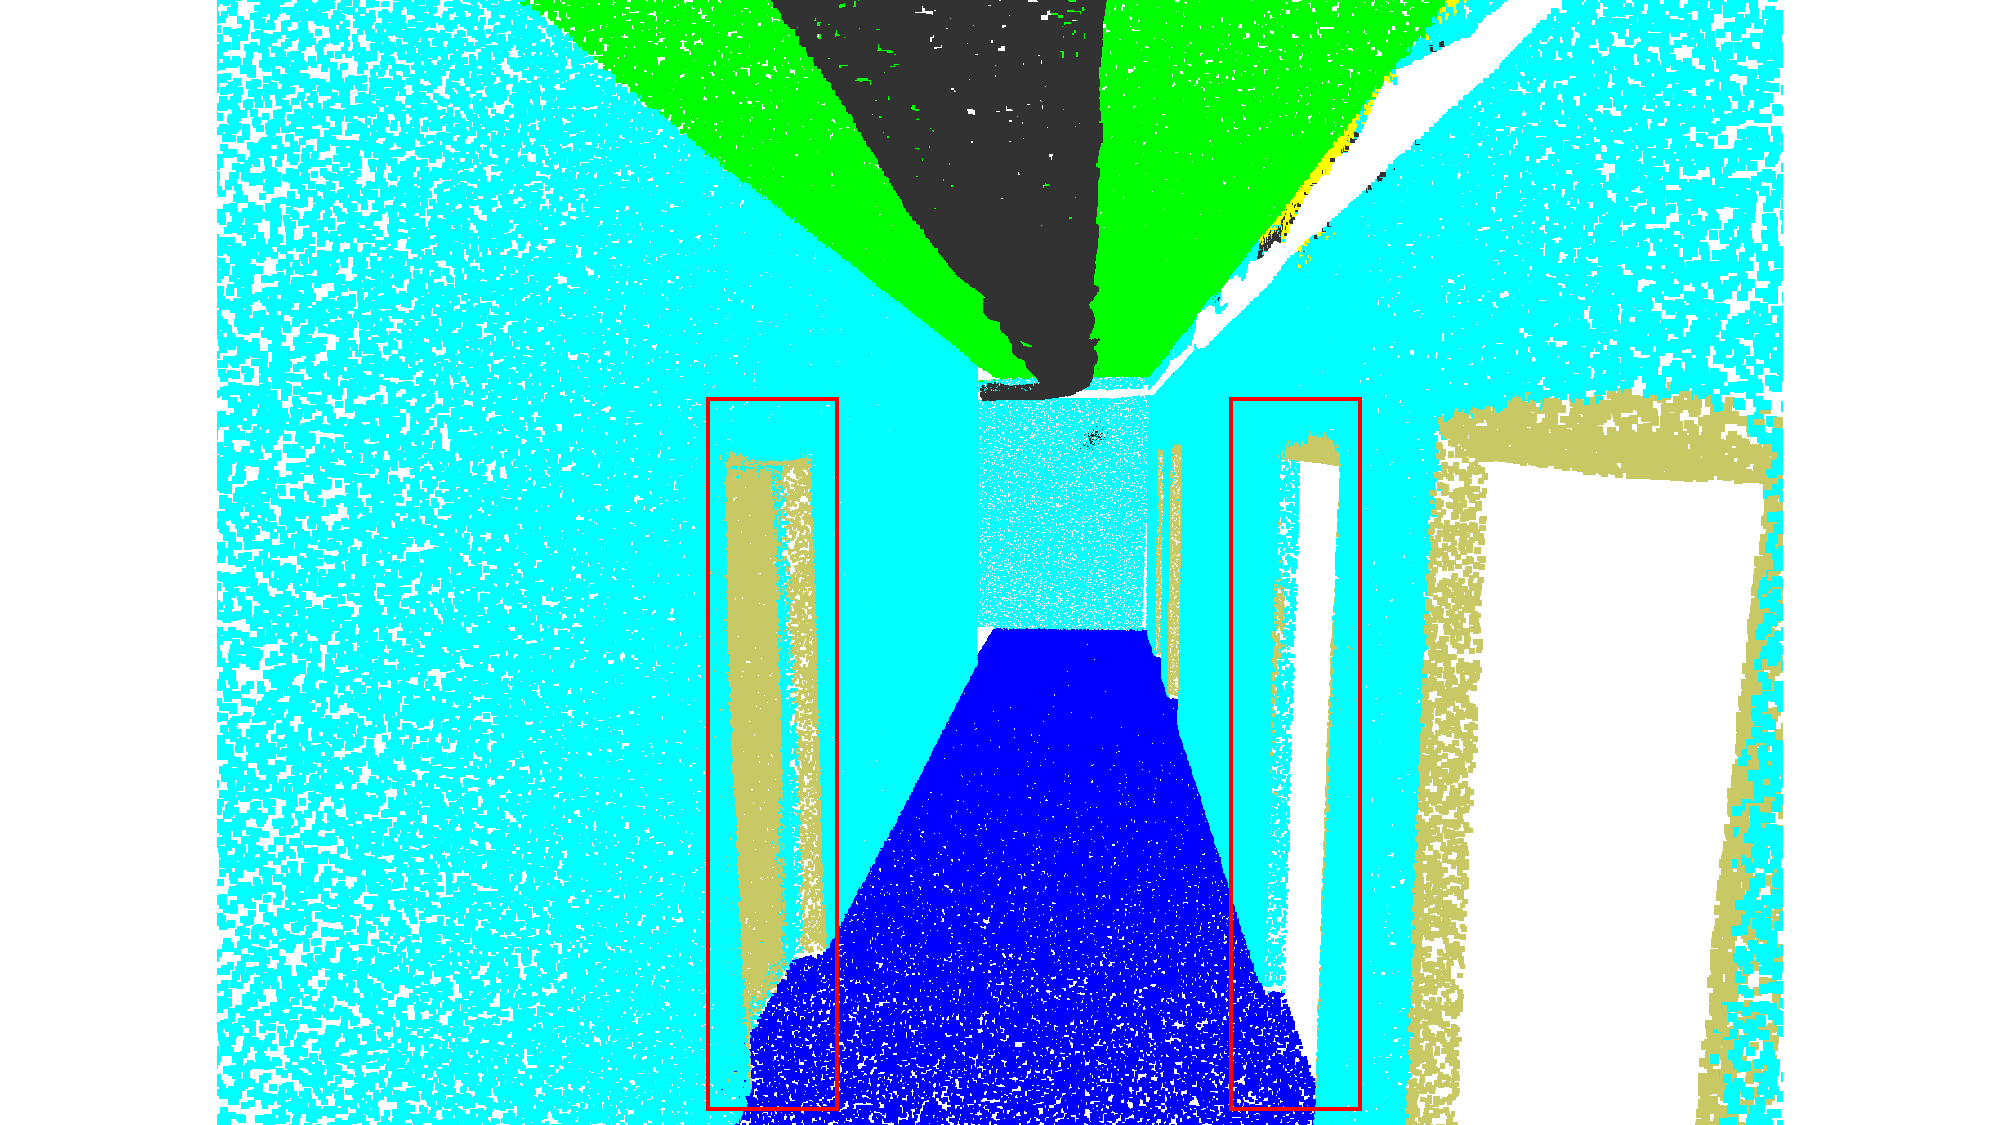
\includegraphics[width=\textwidth]{fig/supplement/semantic_segmentation/hallway_10/PPT_hallway_10.pdf}
    \end{minipage}
    \hfill
    \begin{minipage}{0.22\textwidth}
        \centering
        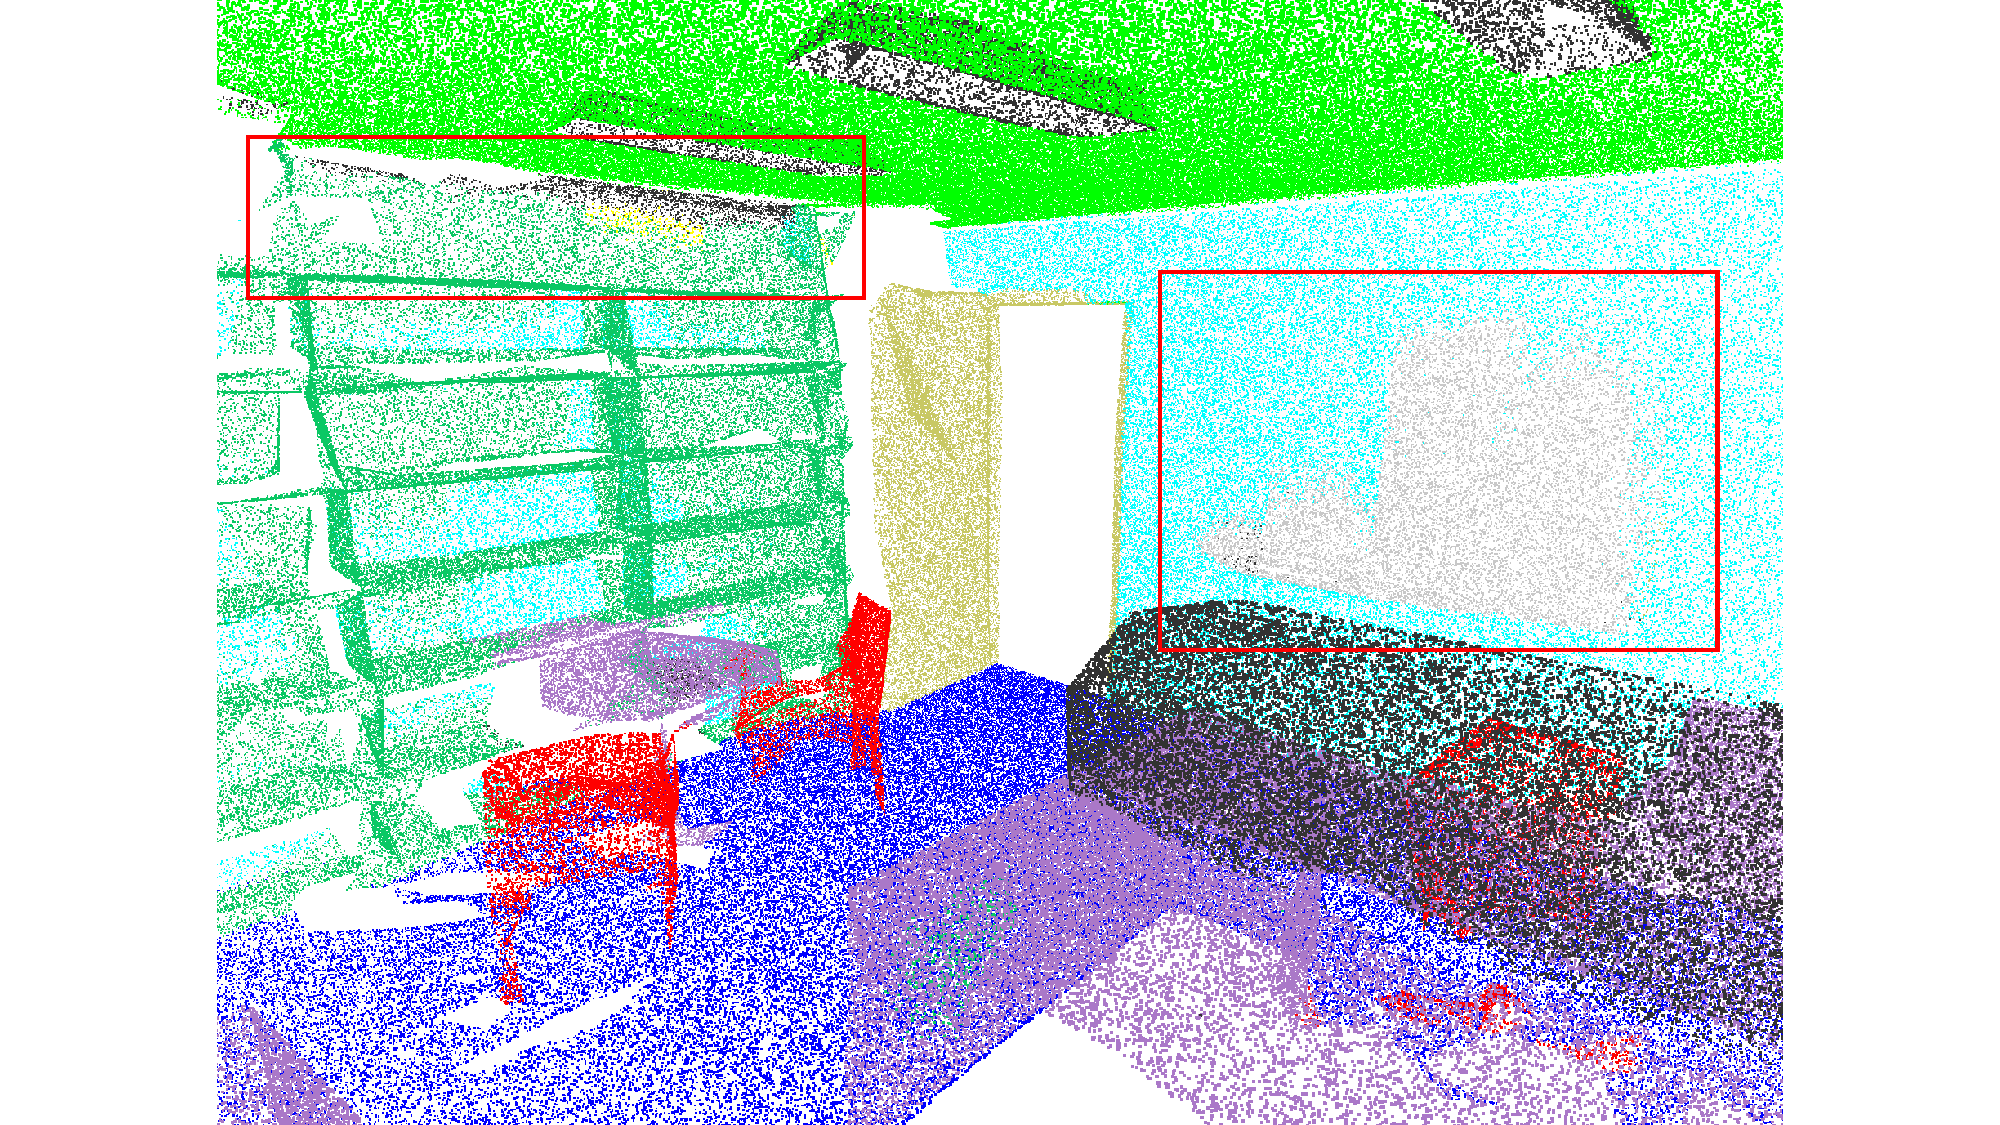
\includegraphics[width=\textwidth]{fig/supplement/semantic_segmentation/office_35/PPT_office_35.pdf}
    \end{minipage}
    \hfill
    \begin{minipage}{0.22\textwidth}
        \centering
        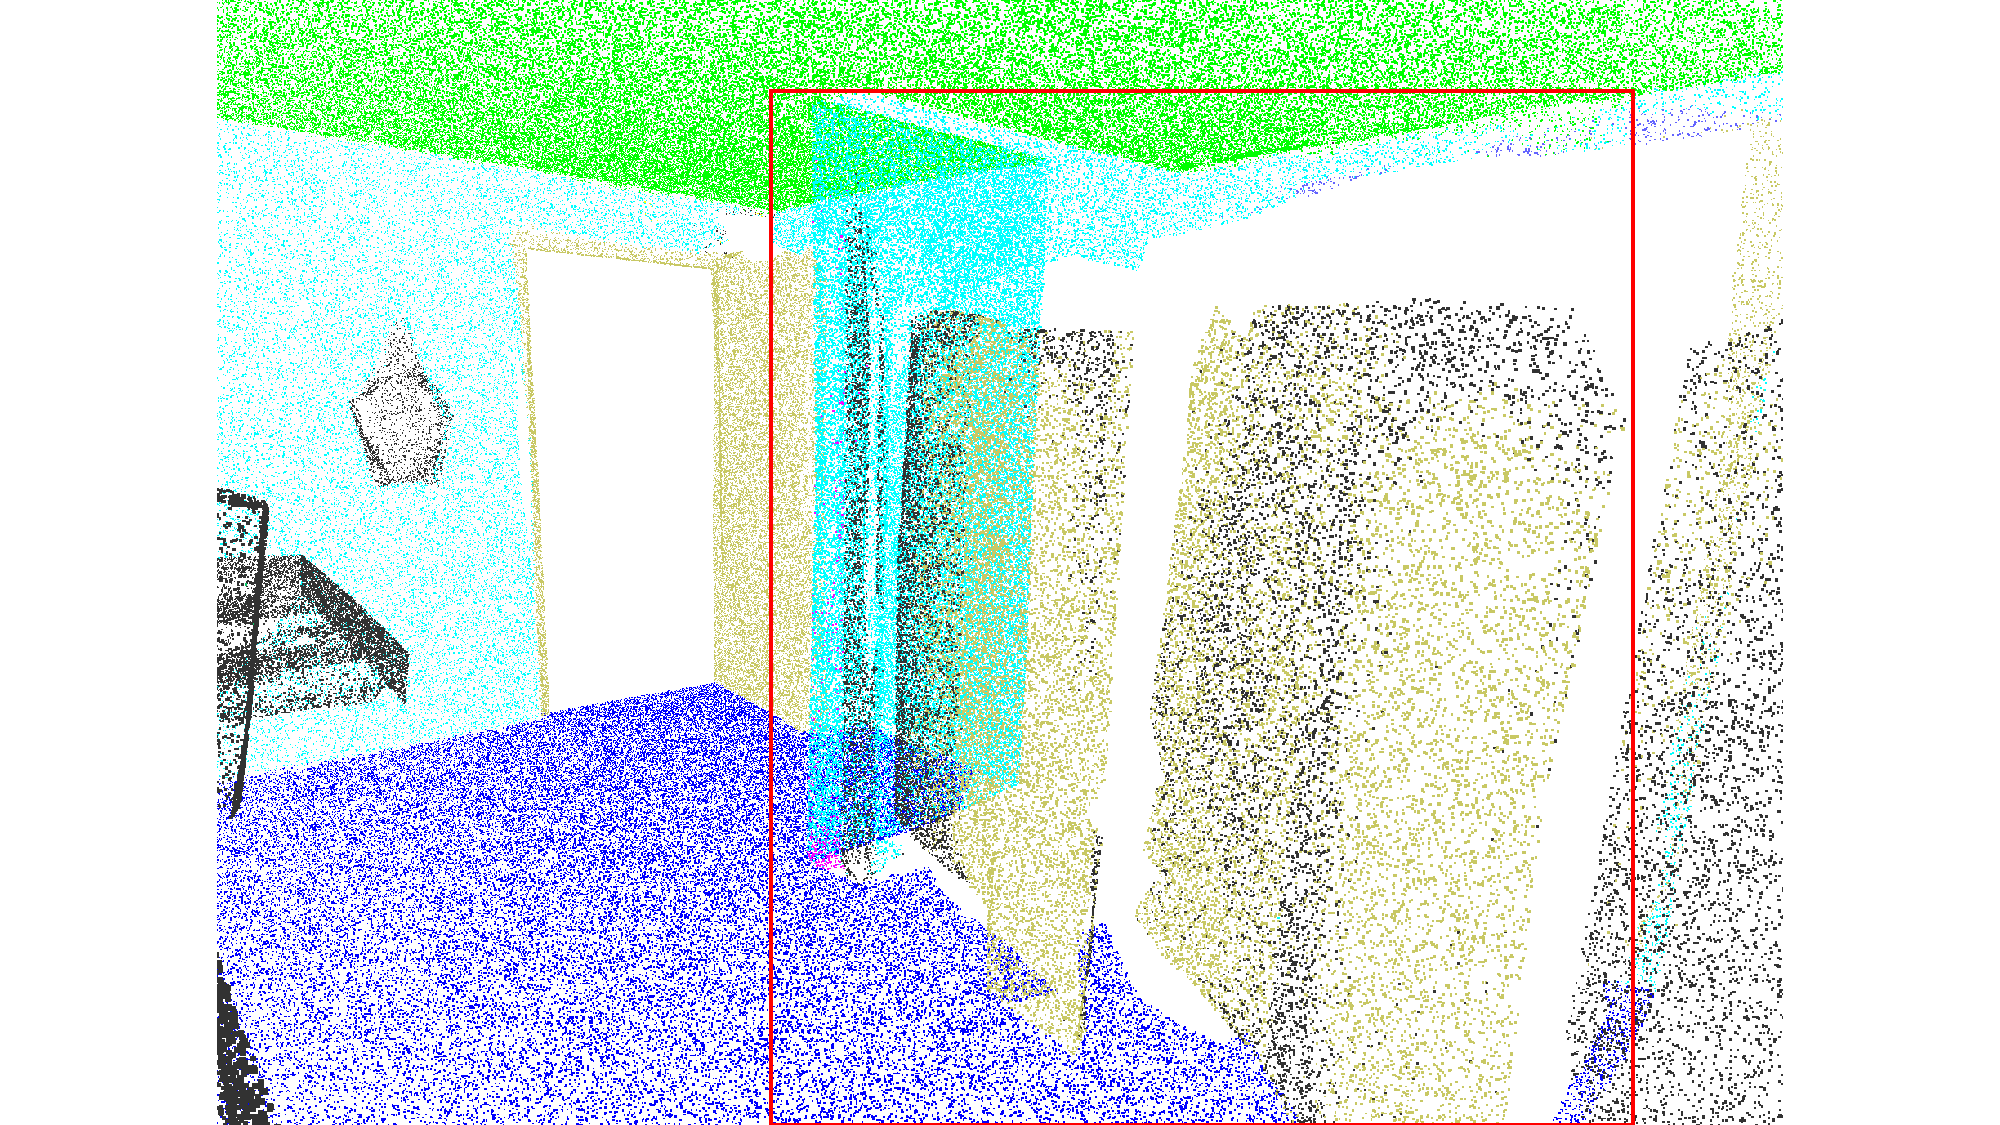
\includegraphics[width=\textwidth]{fig/supplement/semantic_segmentation/wc_2/PPT_wc_2.pdf}
    \end{minipage}
    \hfill

    % 换行
    \vspace{0.5em}

    % 第五行左侧的竖排标签
    \begin{minipage}{0.09\textwidth}
        \centering
        PointGST
    \end{minipage}
    \hfill
    % 第五行图片
    \begin{minipage}{0.22\textwidth}
        \centering
        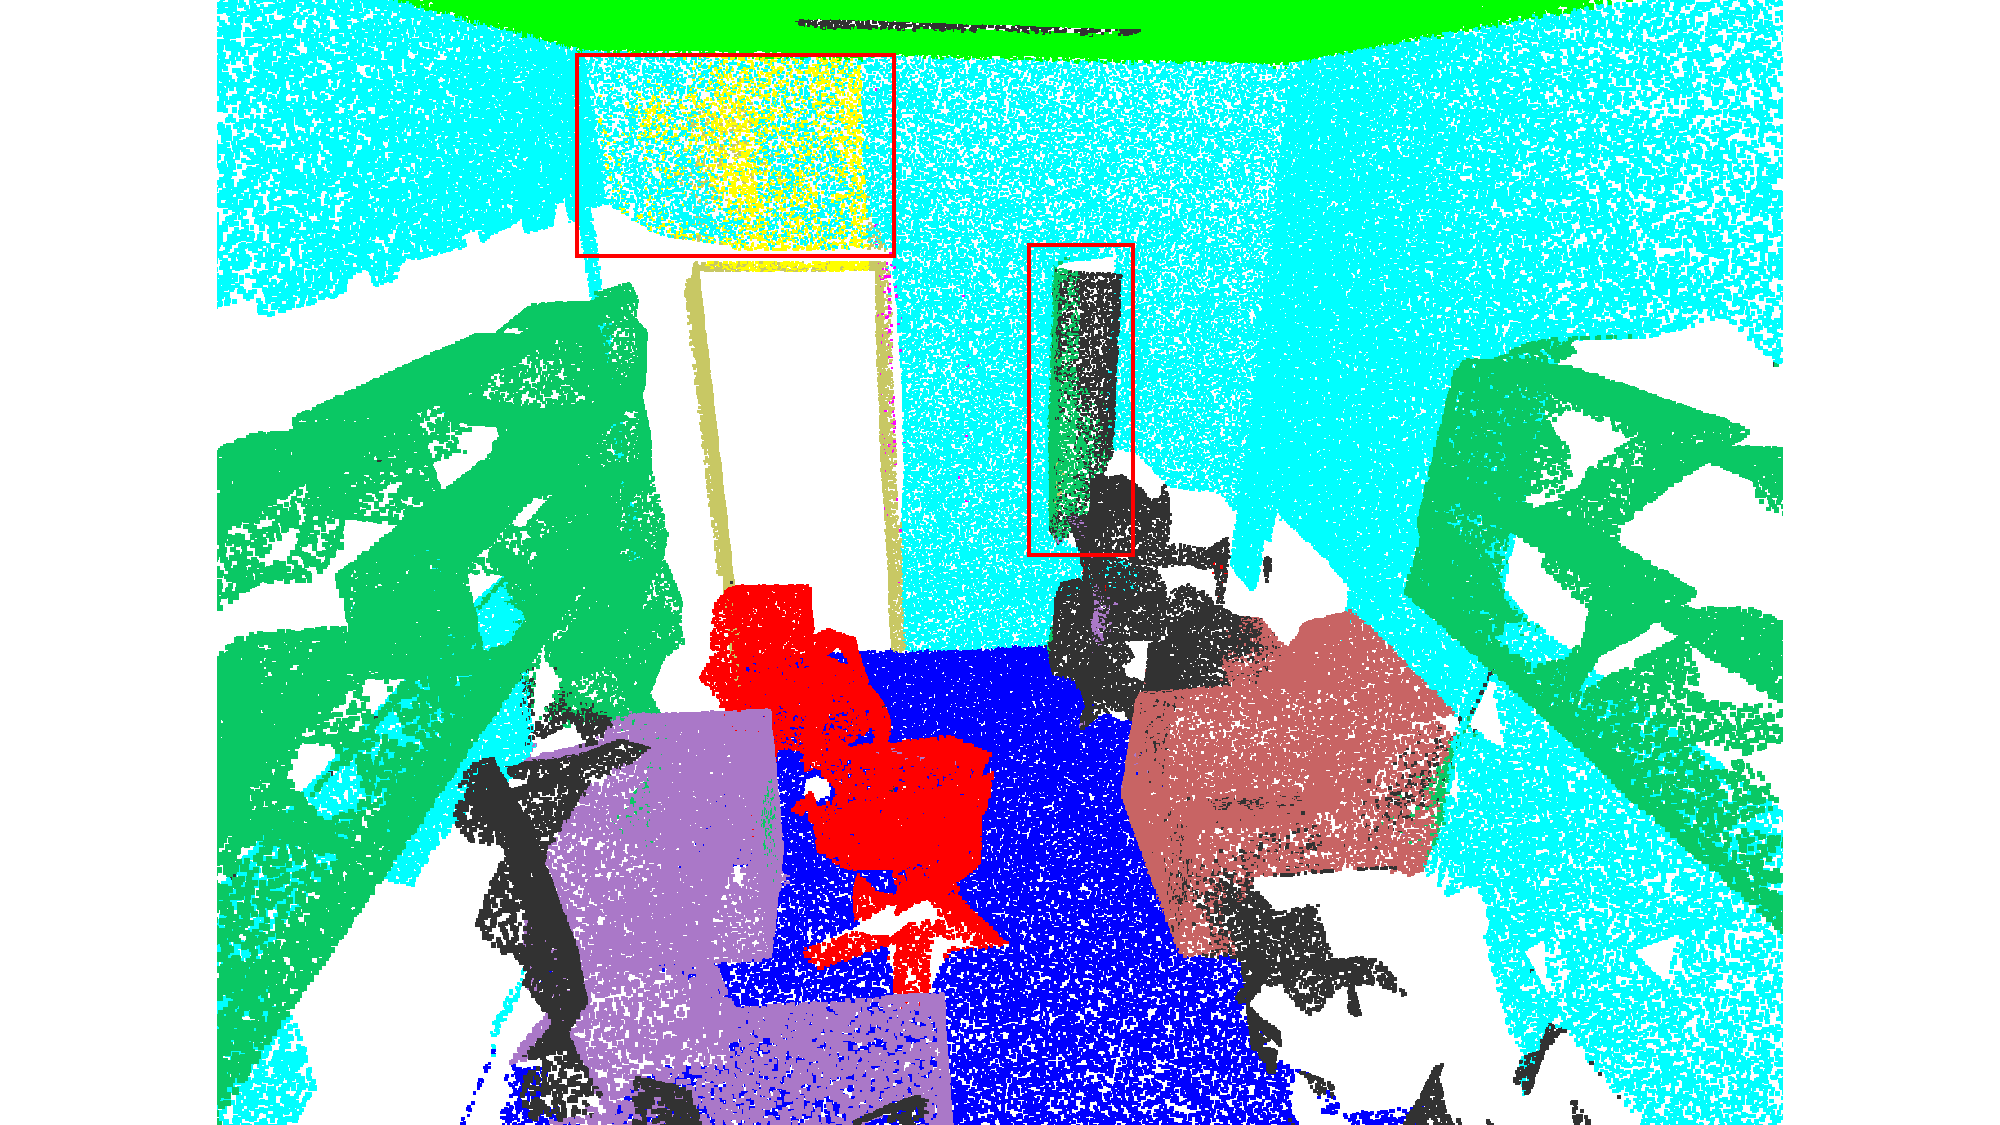
\includegraphics[width=\textwidth]{fig/supplement/semantic_segmentation/office_9/PointGST_office_9.pdf}
    \end{minipage}
    \hfill
    \begin{minipage}{0.22\textwidth}
        \centering
        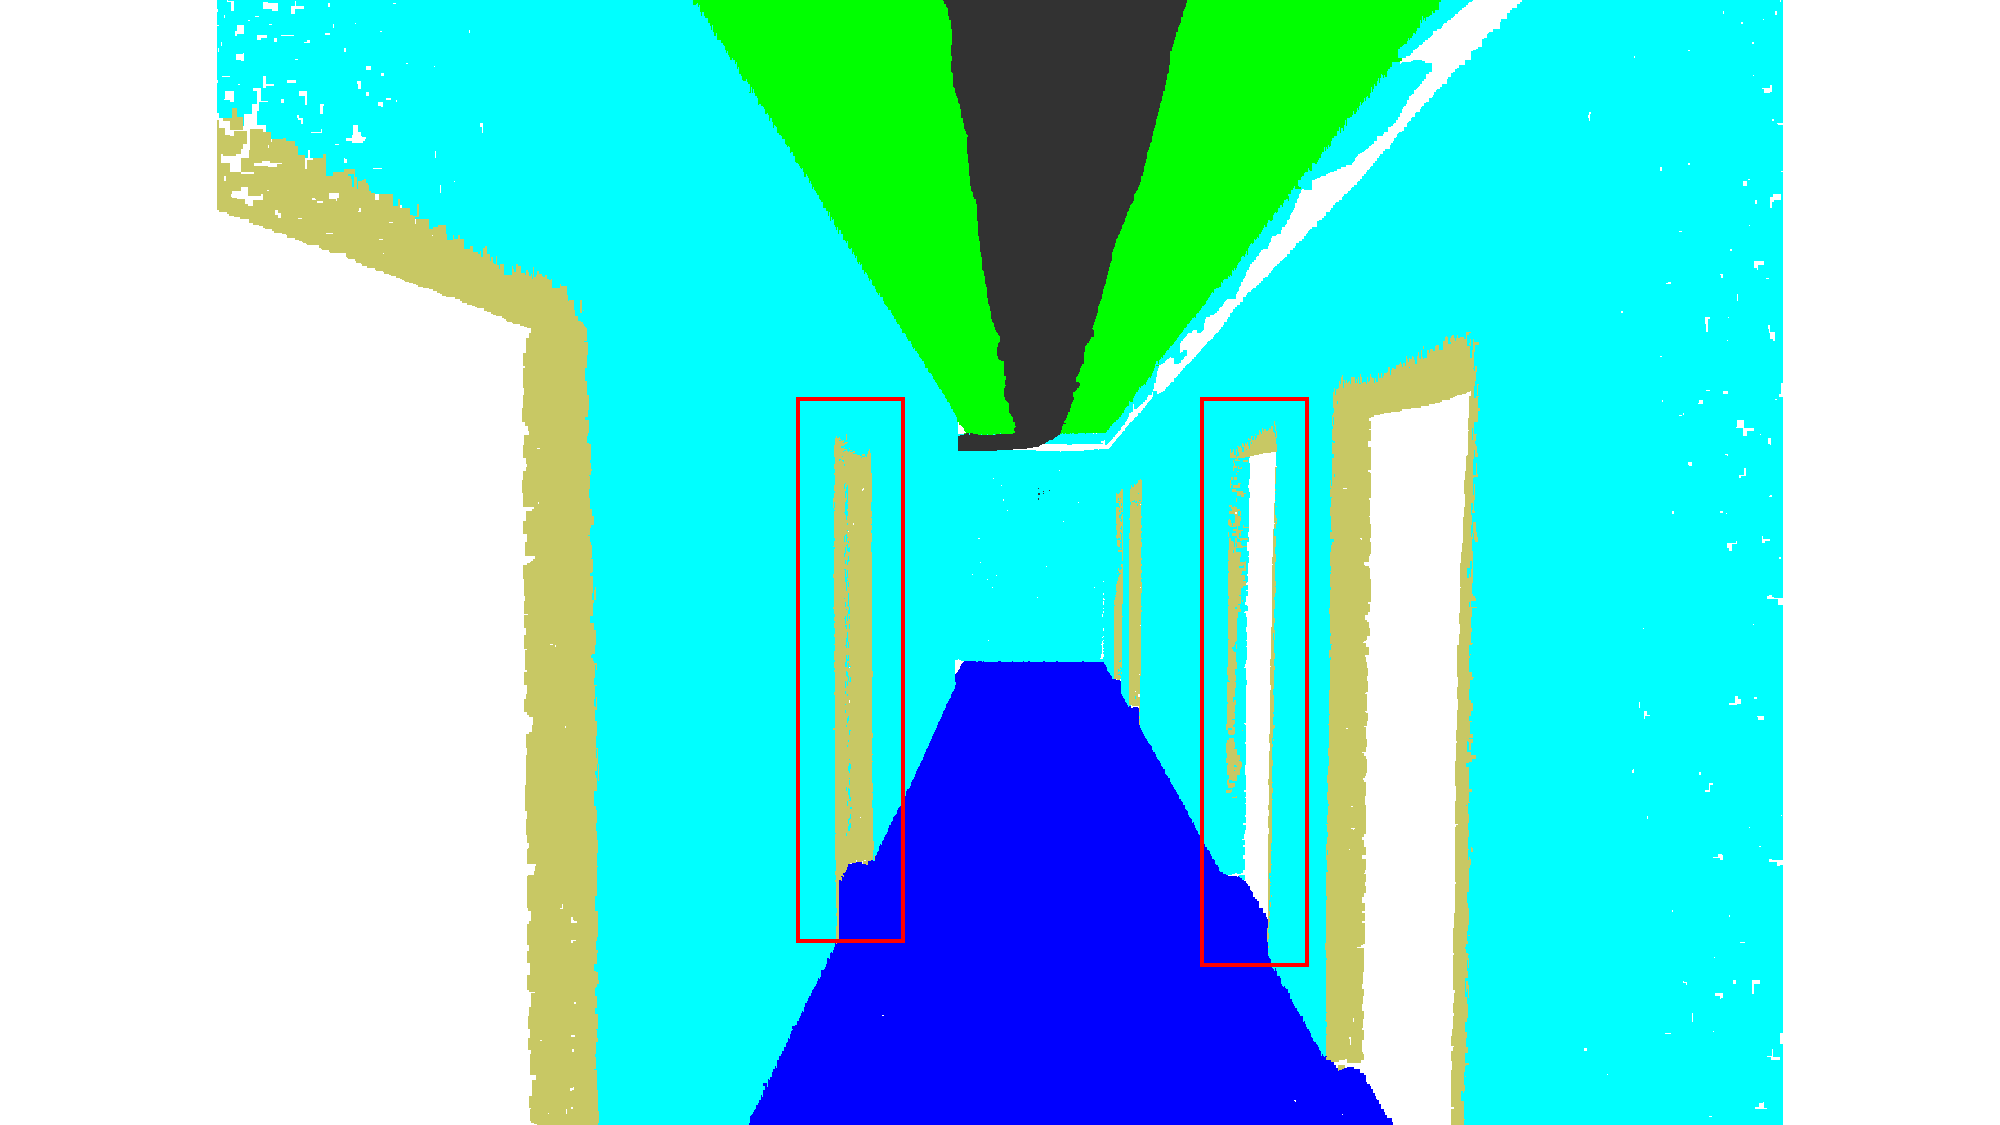
\includegraphics[width=\textwidth]{fig/supplement/semantic_segmentation/hallway_10/PointGST_hallway_10.pdf}
    \end{minipage}
    \hfill
    \begin{minipage}{0.22\textwidth}
        \centering
        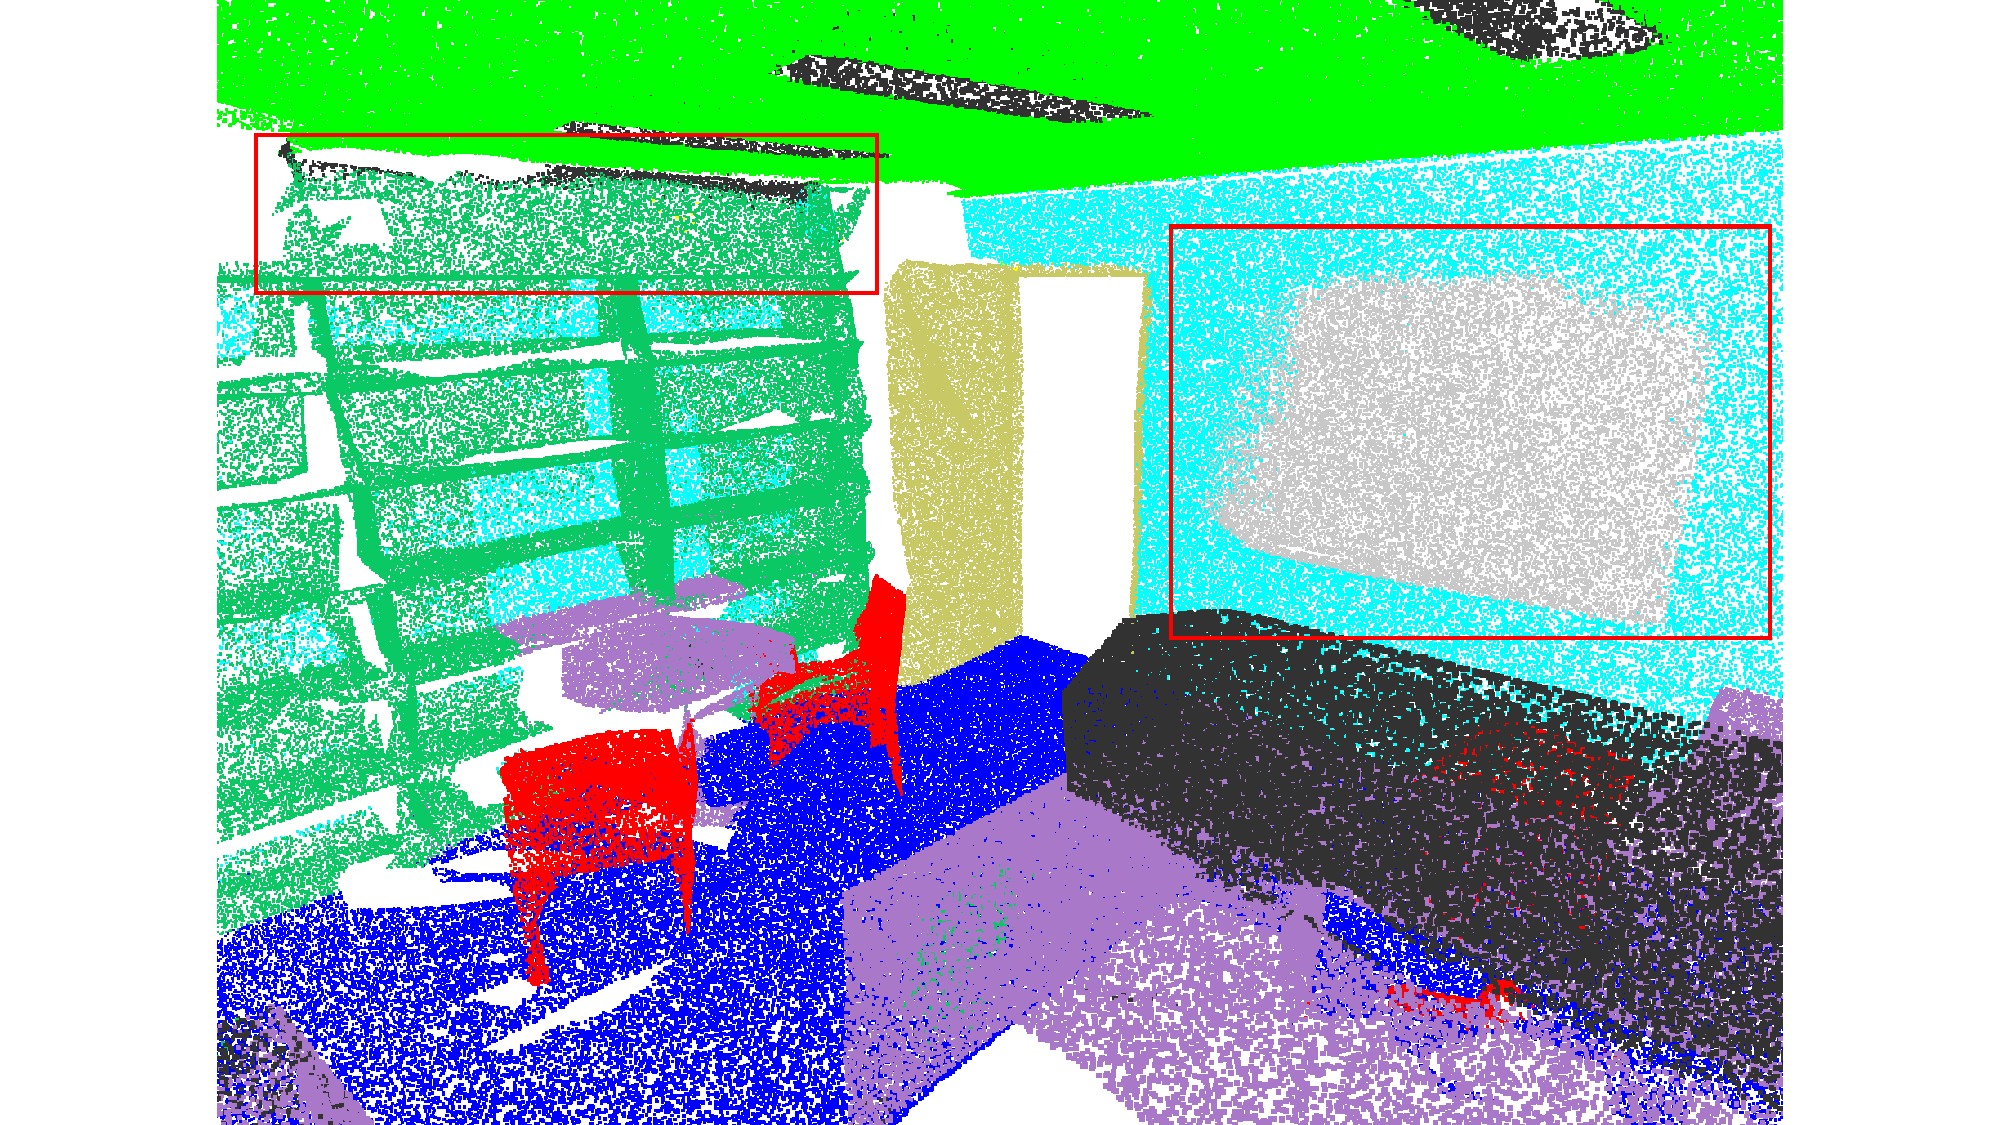
\includegraphics[width=\textwidth]{fig/supplement/semantic_segmentation/office_35/PointGST_office_35.pdf}
    \end{minipage}
    \hfill
    \begin{minipage}{0.22\textwidth}
        \centering
        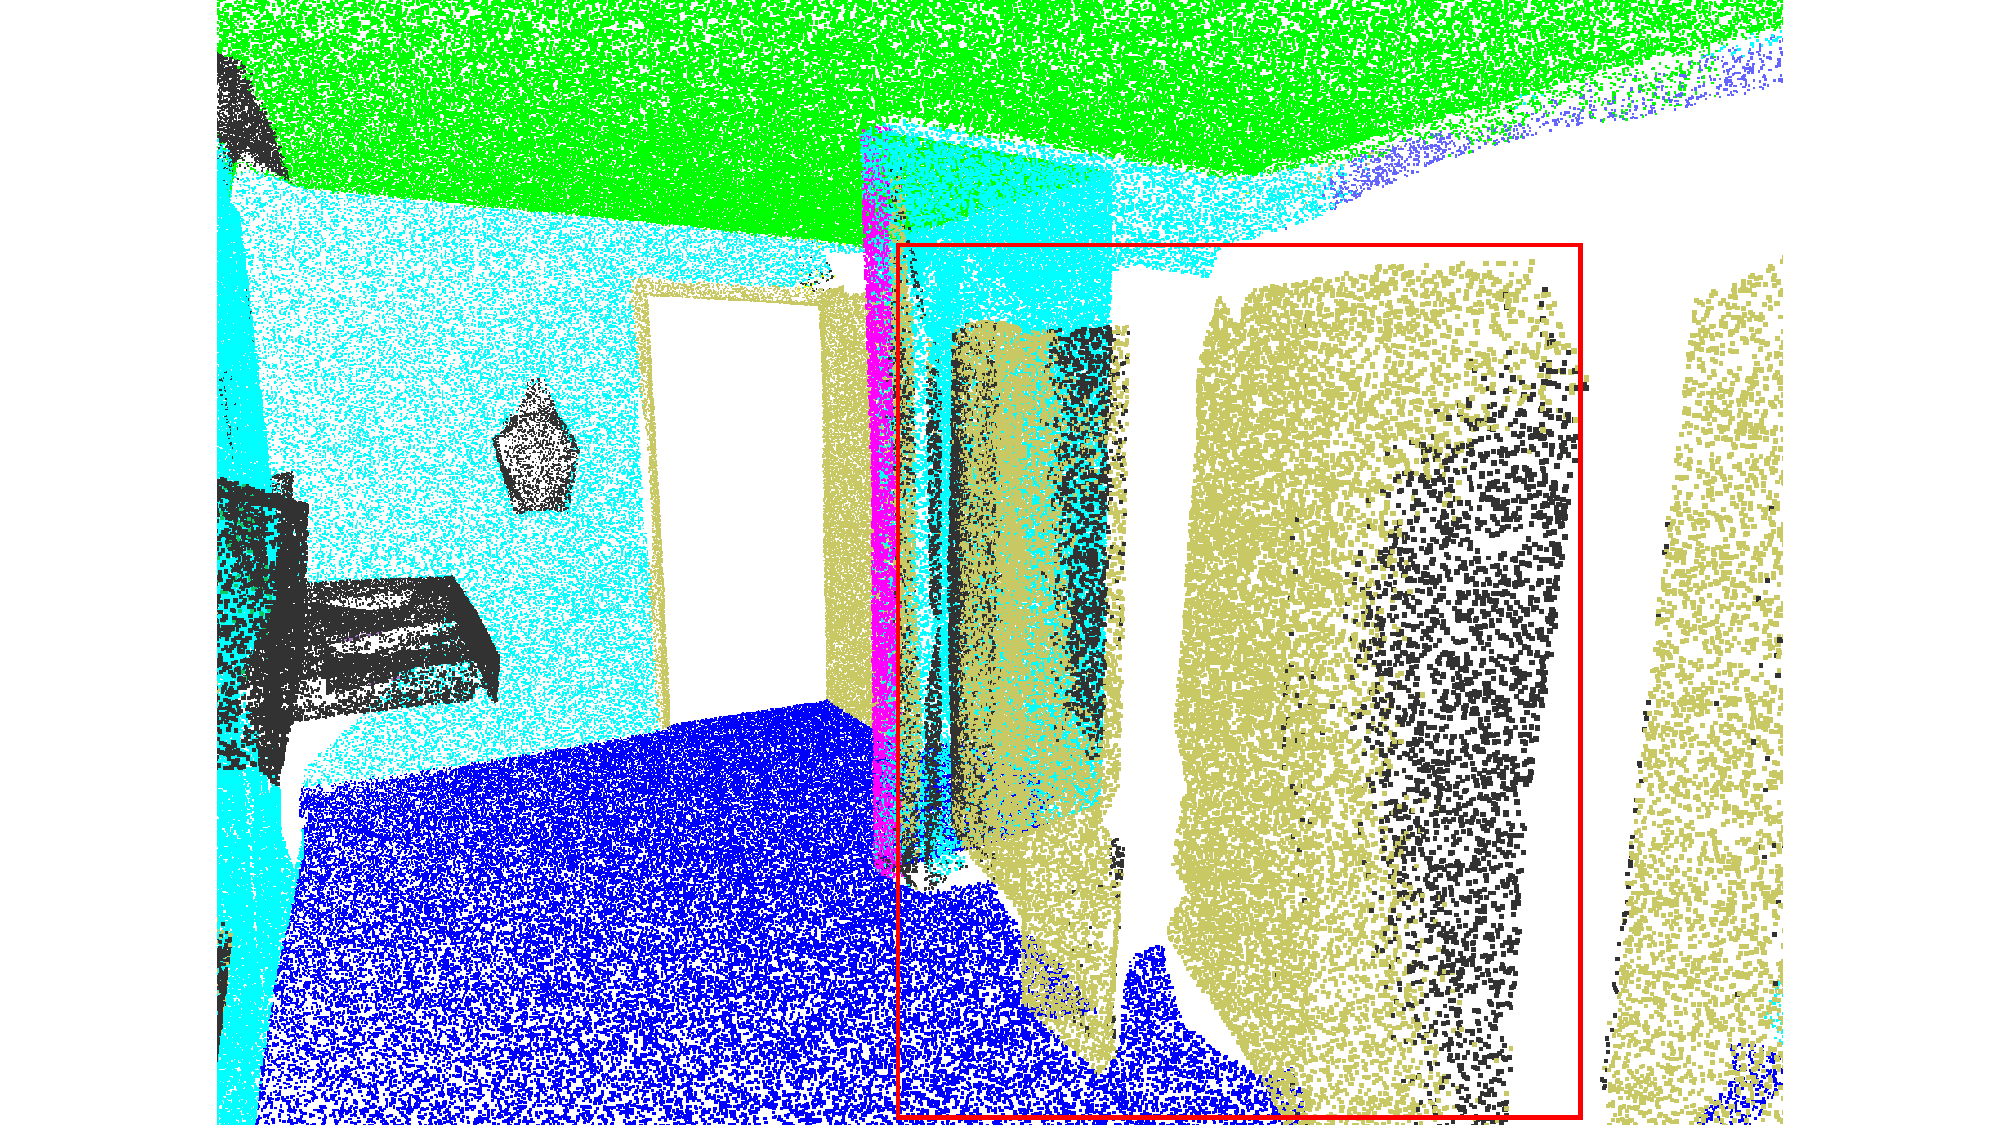
\includegraphics[width=\textwidth]{fig/supplement/semantic_segmentation/wc_2/PointGST_wc_2.pdf}
    \end{minipage}
    \hfill

    % 换行
    \vspace{0.5em}

    % 第六行左侧的竖排标签
    \begin{minipage}{0.09\textwidth}
        \centering
        PLT (Ours)
    \end{minipage}
    \hfill
    % 第六行图片
    \begin{minipage}{0.22\textwidth}
        \centering
        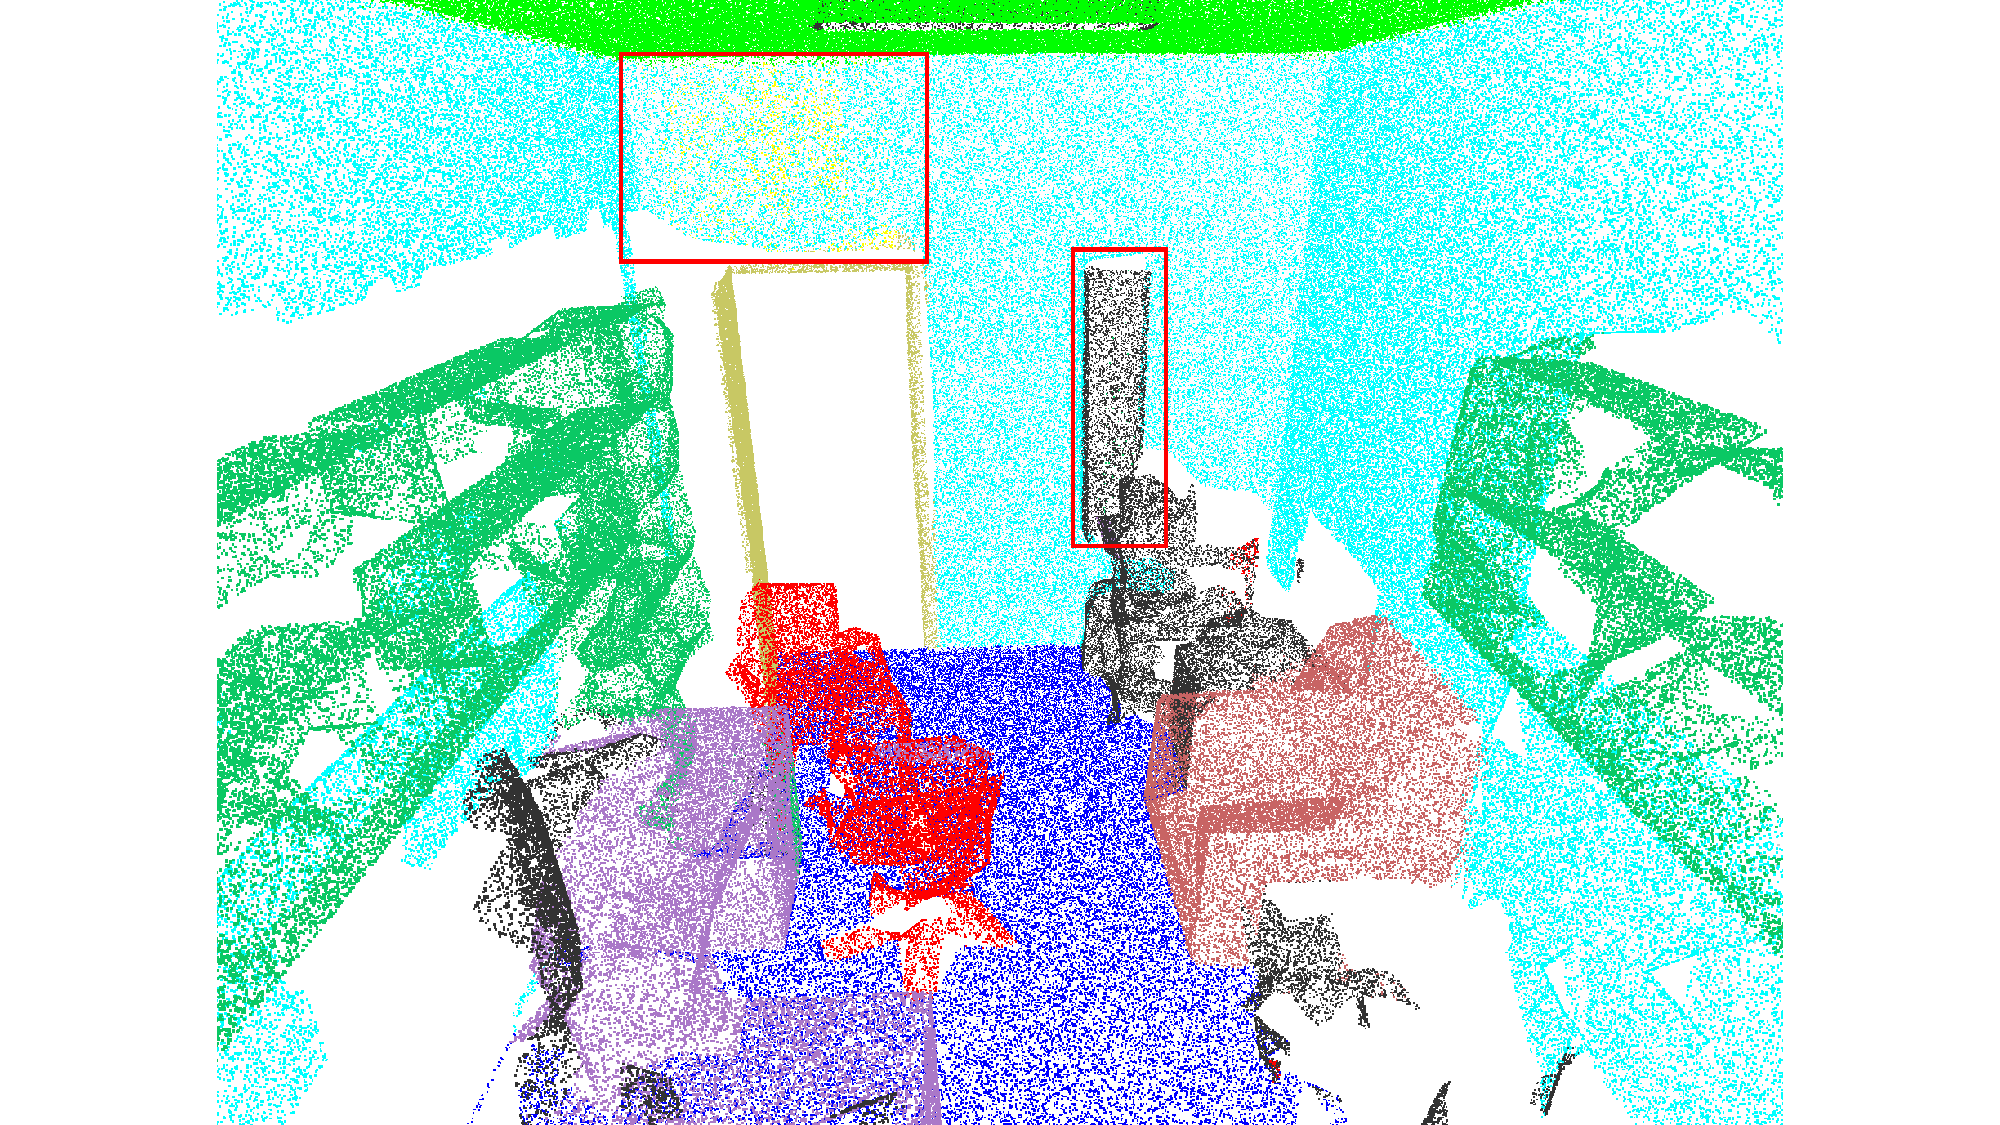
\includegraphics[width=\textwidth]{fig/supplement/semantic_segmentation/office_9/PLT_office_9.pdf}
    \end{minipage}
    \hfill
    \begin{minipage}{0.22\textwidth}
        \centering
        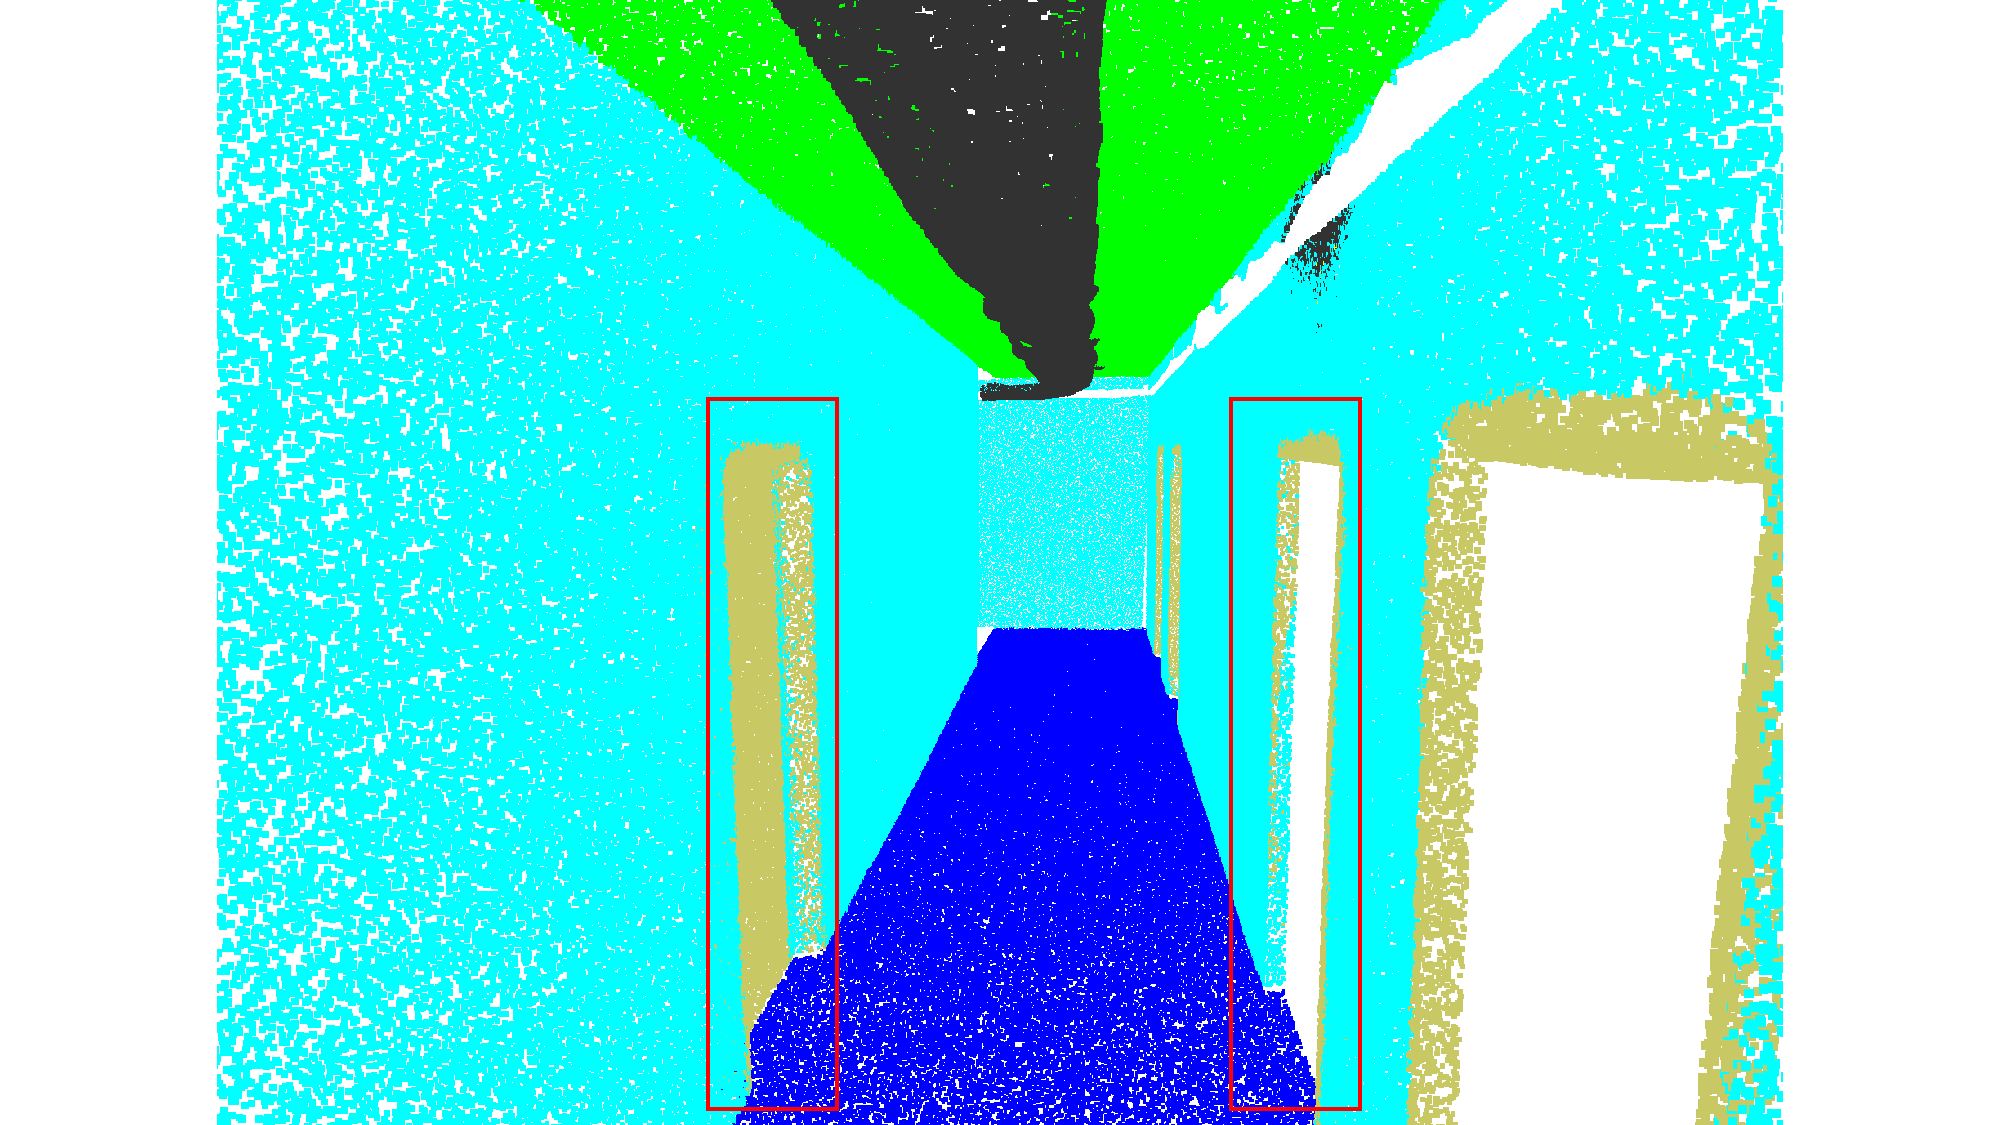
\includegraphics[width=\textwidth]{fig/supplement/semantic_segmentation/hallway_10/PLT_hallway_10.pdf}
    \end{minipage}
    \hfill
    \begin{minipage}{0.22\textwidth}
        \centering
        \includegraphics[width=\textwidth]{fig/supplement/semantic_segmentation/office_35/PLT_office_35.pdf}
    \end{minipage}
    \hfill
    \begin{minipage}{0.22\textwidth}
        \centering
        \includegraphics[width=\textwidth]{fig/supplement/semantic_segmentation/wc_2/PLT_wc_2.pdf}
    \end{minipage}
    \hfill

    % 换行
    \vspace{0.5em}

    % 第七行左侧的竖排标签
    \begin{minipage}{0.09\textwidth}
        \centering
        GT
    \end{minipage}
    \hfill
    % 第七行图片
    \begin{minipage}{0.22\textwidth}
        \centering
        \includegraphics[width=\textwidth]{fig/supplement/semantic_segmentation/office_9/GT_office_9.pdf}
    \end{minipage}
    \hfill
    \begin{minipage}{0.22\textwidth}
        \centering
        \includegraphics[width=\textwidth]{fig/supplement/semantic_segmentation/hallway_10/GT_hallway_10.pdf}
    \end{minipage}
    \hfill
    \begin{minipage}{0.22\textwidth}
        \centering
        \includegraphics[width=\textwidth]{fig/supplement/semantic_segmentation/office_35/GT_office_35.pdf}
    \end{minipage}
    \hfill
    \begin{minipage}{0.22\textwidth}
        \centering
        \includegraphics[width=\textwidth]{fig/supplement/semantic_segmentation/wc_2/GT_wc_2.pdf}
    \end{minipage}
    \hfill
    
    %下方的标签
    \vspace{0.5em}
    \begin{minipage}{0.09\textwidth} % 左侧空白区域
        \color{white}{12}
    \end{minipage}
    \hfill
    \begin{minipage}{0.22\textwidth} % 第2列标题
        \centering
        office\_9
    \end{minipage}
    \hfill
    \begin{minipage}{0.22\textwidth} % 第1列标题
        \centering
        hallway\_10
    \end{minipage}
    \hfill
    \begin{minipage}{0.22\textwidth} % 第3列标题
        \centering
        office\_35
    \end{minipage}
    \hfill
    \begin{minipage}{0.22\textwidth} % 第3列标题
        \centering
        wc\_2
    \end{minipage}
    \hfill
    \caption{The visualization of qualitative results for point cloud semantic segmentation. We compare our PLT with previous methods on Area 5 of the S3DIS dataset~\cite{armeni20163d}.}
    \label{fig:s3dis_1}

\end{figure*}

